\documentclass[oneside, a4paper, 12pt]{memoir}

\usepackage[utf8]{inputenc}
\usepackage[usenames,dvipsnames,svgnames,table]{xcolor}
\usepackage[marginparwidth=28mm]{geometry}
\usepackage[pdftex]{graphicx}
\usepackage{tikz}

\usepackage{filecontents}
\usepackage[T1]{fontenc}
\usepackage[UKenglish]{babel}
\usepackage{newpxtext,newpxmath}
\usepackage[babel=true]{csquotes}
\usepackage[round]{natbib}
%\usepackage[colorinlistoftodos]{todonotes}
\usepackage{comment}
\usetikzlibrary{arrows,automata,external}
\tikzexternalize[prefix=tikz_external_figures/]
\usepackage{ccaption}
%\usepackage{flafter}
\usepackage{pgfplots}
\pgfplotsset{compat=1.12}
\usepackage[figure]{algorithm2e}
\usepackage[hidelinks,breaklinks=true]{hyperref}
\usepackage[section]{placeins}

% Logos
\newcommand{\ulb}{
\includegraphics[scale=1.1]{PageDeGarde_MFE/logo_ULB2.pdf}}
\newcommand{\polytech}{
\includegraphics[scale=0.35]{PageDeGarde_MFE/logo_polytech_FR.pdf}}

% Polices
\definecolor{ULBblue}{rgb}{0,0.2196,0.5765}
\newcommand{\fontTitle}{\sffamily \Huge\selectfont \color{ULBblue}}
\newcommand{\fontSubtitle}{\sffamily \LARGE \selectfont \color{ULBblue}}
\newcommand{\fontText}{\sffamily \selectfont}
\newcommand{\fontColor}{\sffamily \selectfont \color{ULBblue}}

% Titre
\newcommand{\titleA}{\fontTitle{Human - Robots Swarms Interaction}} % Titre identique au titre remis au secrétariat
%\newcommand{\titleB}{\fontTitle{Deuxième ligne de titre du mémoire}} % (dans la langue de rédaction a priori)
% Sous-titre
\newcommand{\subtitleA}{\fontSubtitle{An Escorting Robot Swarm that Diverts a Human}}
\newcommand{\subtitleB}{\fontSubtitle{away from Dangers one cannot perceive.}}
% Titre du diplôme
\newcommand{\diplomaA}{\fontText{Mémoire présenté en vue de l’obtention du diplôme}} % A laisser en Français
\newcommand{\diplomaB}{\fontText{d'Ingénieur Civil en Informatique à finalité Intelligence Computationnelle}}

% Etudiant
\newcommand{\student}{\textbf{\sffamily \large Anthony Debruyn}}

% Supervision
\newcommand{\promAa}{\fontColor{Directeur}}
\newcommand{\promAb}{\fontText{Professeur Mauro Birattari}}
\newcommand{\promBa}{\fontColor{Co-Promoteur}}
\newcommand{\promBb}{\fontText{Professeur Marco Dorigo}}
\newcommand{\promCa}{\fontColor{Superviseurs}}
\newcommand{\promCb}{\fontText{Gaëtan Podevijn, Andreagiovanni Reina}}
\newcommand{\deptA}{\fontColor{Service}}
\newcommand{\deptB}{\fontText{IRIDIA}}

% Année académique
\newcommand{\yearA}{\fontColor{Année académique}}
\newcommand{\yearB}{\fontText{2014 - 2015}}

%%%%%%%%%%%%%%%%%%%%%%%%%%%%%%%%%%%%%%%%%%%%%%%%%%%%%%%
% MY NEW COMMANDS
%%%%%%%%%%%%%%%%%%%%%%%%%%%%%%%%%%%%%%%%%%%%%%%%%%%%%%%

\newcommand{\quoto}[2]{
\begin{quotation}
\textit{\enquote{#1} - #2}
\end{quotation}
}

\newcommand{\quot}[1]{\textit{\enquote{#1}}}


\newcommand{\epuck}[3][0] % [angle]{x}{y} avec angle optionel
{
	\draw [very thick, fill=white] (#2,#3) circle [radius=0.5];
	\draw [very thick, rotate around={#1:(#2,#3)}] (#2-0.25,#3-0.433) -- (#2,#3+0.45) -- (#2+0.25,#3-0.433);
}

\newcommand{\epuckred}[3][0] % [angle]{x}{y} avec angle optionel
{
	\draw [very thick, fill=orange] (#2,#3) circle [radius=0.5];
	\draw [very thick, rotate around={#1:(#2,#3)}] (#2-0.25,#3-0.433) -- (#2,#3+0.45) -- (#2+0.25,#3-0.433);
}

\newcommand{\epuckblue}[3][0] % [angle]{x}{y} avec angle optionel
{
	\draw [very thick, fill=RoyalBlue] (#2,#3) circle [radius=0.5];
	\draw [very thick, rotate around={#1:(#2,#3)}] (#2-0.25,#3-0.433) -- (#2,#3+0.45) -- (#2+0.25,#3-0.433);
}

\newcommand{\human}[3][0] % [angle]{x}{y}
{
	\draw [very thick, fill=white, rotate around={#1:(#2,#3)}] (#2-1,#3+0.5) ellipse (0.25cm and 0.5cm);
	\draw [very thick, fill=white, rotate around={#1:(#2,#3)}] (#2+1,#3+0.5) ellipse (0.25cm and 0.5cm);
	\draw [very thick, fill=white, rotate around={#1:(#2,#3)}] (#2,#3) ellipse (1.5cm and 0.75cm);
	\draw [thick, fill=white, rotate around={#1:(#2,#3)}] (#2-0.05,#3+1) -- (#2,#3+1.1) -- (#2+0.05,#3+1);
	\draw [very thick, fill=white, rotate around={#1:(#2,#3)}] (#2,#3+0.5) circle [radius=0.5cm];
}


\let\oldCaption\caption
\renewcommand{\caption}[2]{
\oldCaption[#1]{{\small\sffamily\bfseries #1:} #2}
}

%%%%%%%%%%%%%%%%%%%%%%%%%%%%%%%%%%%%%%%%%%%%%%%%%%%%%%%
% NEW STYLES
%%%%%%%%%%%%%%%%%%%%%%%%%%%%%%%%%%%%%%%%%%%%%%%%%%%%%%%

\captiondelim{ -- }
\captionnamefont{\small\sffamily\bfseries}
\captiontitlefont{\small\sffamily}
\precaption{\rule{\linewidth}{0.4pt}\\}
%\setcounter{secnumdepth}{3}
%\setcounter{tocdepth}{3}
\maxsecnumdepth{subsubsection}% 'secnumdepth' is reset by \mainmatter. You should use 'maxsecnumdepth'.
\maxtocdepth{subsection}

\setlength\parskip{\baselineskip}

%%%%%%%%%%%%%%%%%%%%%%%%%%%%%%%%%%%%%%%%%%%%%%%%%%%%%%%
% THE DOCUMENT
%%%%%%%%%%%%%%%%%%%%%%%%%%%%%%%%%%%%%%%%%%%%%%%%%%%%%%%

\begin{document}
\frontmatter

	\thispagestyle{empty}
	\newgeometry{top=2.5cm, bottom=1.5cm, left=2.5cm, right=1cm}
	\setlength{\unitlength}{1mm}
	\noindent\begin{picture}(175,257)
	
		\put(0,245){\polytech}
		\put(153,139.5){\ulb}
		
		\put(8,155){\makebox(150,10)[l]{\titleA}}
%		\put(8,145){\makebox(150,10)[l]{\titleB}}
		\put(8,135){\makebox(150,10)[l]{\subtitleA}}
		\put(8,125){\makebox(150,10)[l]{\subtitleB}}
		
		\put(0,75){
		\begin{tikzpicture}[scale=0.1]
		\fill [fill=ULBblue](0,0) rectangle (0.8,90);
		\fill [fill=ULBblue](0,47) rectangle (152,47.8);
		\end{tikzpicture}}
		
		\put(8,110){\makebox(150,5)[l]{\diplomaA}}
		\put(8,105){\makebox(150,5)[l]{\diplomaB}}
		
		\put(8,75){\makebox(150,10)[l]{\selectfont \student}}
		
		\put(8,44){\makebox(80,5)[l]{\promAa}}
		\put(8,39){\makebox(80,5)[l]{\promAb}}
		\put(8,31){\makebox(80,5)[l]{\promBa}} % Commenter la ligne si pas nécessaire
		\put(8,26){\makebox(80,5)[l]{\promBb}} % Commenter la ligne si pas nécessaire
		\put(8,18){\makebox(80,5)[l]{\promCa}} % Commenter la ligne si pas nécessaire
		\put(8,13){\makebox(80,5)[l]{\promCb}} % Commenter la ligne si pas nécessaire
		\put(8,5){\makebox(80,5)[l]{\deptA}}
		\put(8,0){\makebox(80,5)[l]{\deptB}}
		
		\put(145,5){\makebox(30,5)[r]{\yearA}}
		\put(145,0){\makebox(30,5)[r]{\yearB}}
	
	\end{picture}
	\restoregeometry
	
% Template conçu par Benjamin Vanhemelryck et revu par François Bronchart - Mai 2013
	
%%%%%%%%%%%%%%%%%%%%%%%%%%%%%%%%%%%%%%%%%%%%%%%%%%%%%%%
% BEFORE TEXT
%%%%%%%%%%%%%%%%%%%%%%%%%%%%%%%%%%%%%%%%%%%%%%%%%%%%%%%
\addcontentsline{toc}{part}{First Matter}
\part*{First Matter}
\chapter{Acknowledgements}

\begin{figure}[!htp]
	\centering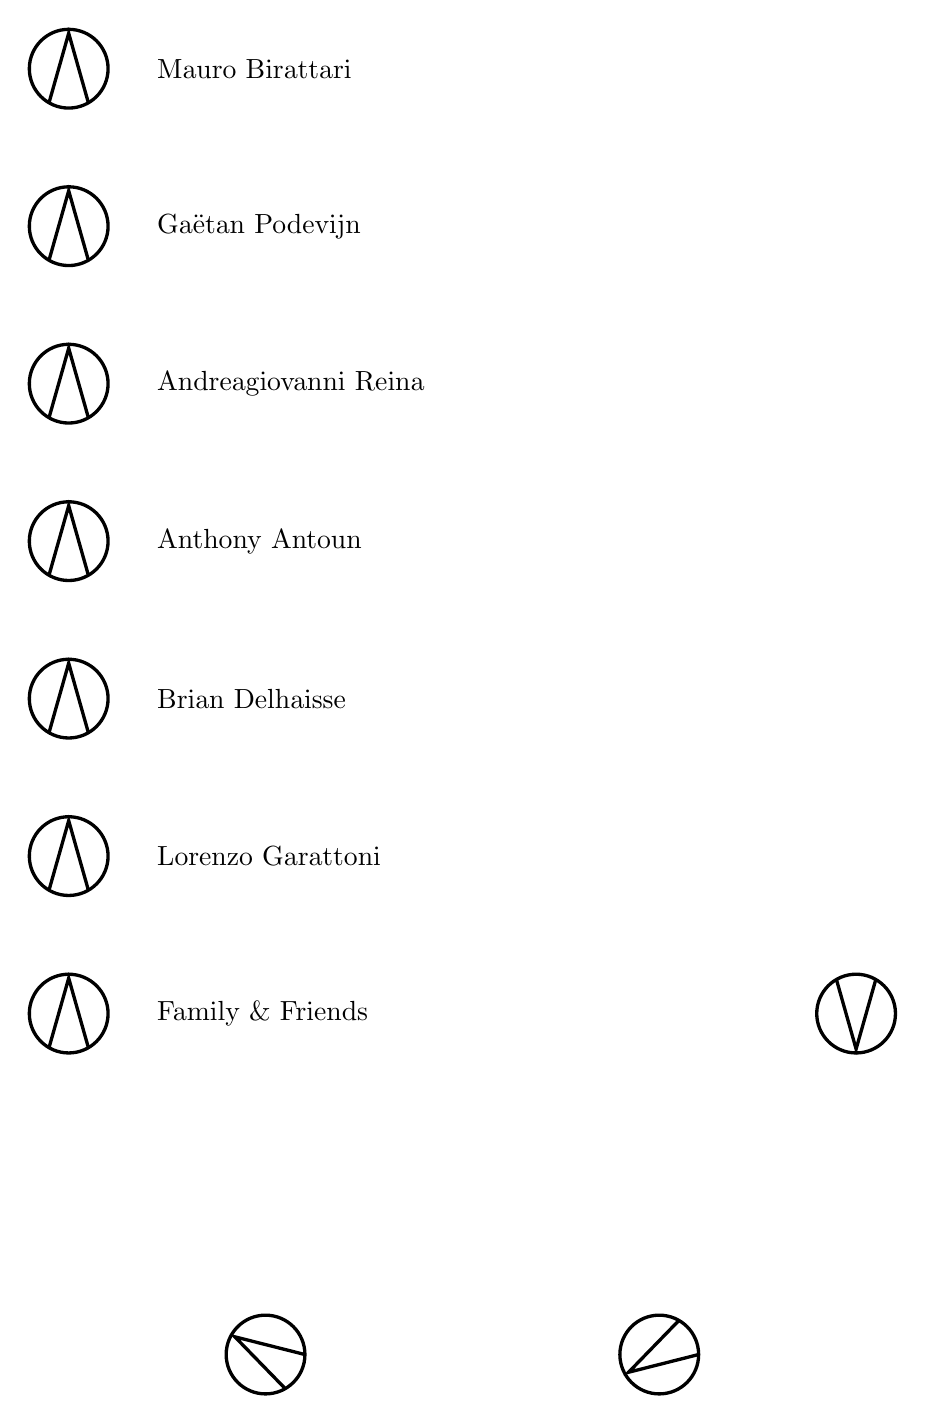
\begin{tikzpicture}
	%Mauro, Gaëtan, Giovanni, Anthony, Lorenzo, Brian, Family and friends.
	\epuck{-5}{12}
	\epuck{-5}{10}
	\epuck{-5}{8}
	\epuck{-5}{6}
	\epuck{-5}{4}
	\epuck{-5}{2}
	\epuck{-5}{0}
	\epuck[60]{-2.5}{-4.33}
	\epuck[120]{2.5}{-4.33}
	\epuck[180]{5}{0}
	
	\draw (-4,12) node[anchor=west] {Mauro Birattari};
	\draw (-4,10) node[anchor=west] {Gaëtan Podevijn};
	\draw (-4,8) node[anchor=west] {Andreagiovanni Reina};
	\draw (-4,6) node[anchor=west] {Anthony Antoun};
	\draw (-4,4) node[anchor=west] {Brian Delhaisse};
	\draw (-4,2) node[anchor=west] {Lorenzo Garattoni};
	\draw (-4,0) node[anchor=west] {Family \& Friends};
	
	\end{tikzpicture}
\end{figure}

\chapter{Résumé}
\chapter{Summary}
\tableofcontents
\listoffigures
\listoftables

%\listoftodos

%%%%%%%%%%%%%%%%%%%%%%%%%%%%%%%%%%%%%%%%%%%%%%%%%%%%%%%
% TEXT
%%%%%%%%%%%%%%%%%%%%%%%%%%%%%%%%%%%%%%%%%%%%%%%%%%%%%%%
\part*{Main Matter}
\addcontentsline{toc}{part}{Main Matter}
\mainmatter
\chapter{Introduction}

[I'll do this and this... blah blah blah... Overview and roadmap. The problem is given in the introduction, so we can put the SOA right after, before the detailed description of the problem.]

\begin{comment}
INTRO
Il faut respecter un fil conducteur dans la thèse. D'abord teaser le contenu dans l'introduction : "j'ai fait un super controller qui peut permettre à des robots de protéger un humain. Ca n'avait jamais été fait avant. J'utilise une swarm. J'ai de très bons résultats. On a testé avec des vrais robots, et l'humain est empêché d'accéder à des zones dangereuses.

STATE OF THE ART
Voici ce qui existe dans le domaine human - robot interaction. Rien de tout cela ne me satisfait et répond à mon problème.

Idem pour human - swarm interaction.

Je vais donc essayer de répondre au problème avec une nouvelle solution... Elle est meilleure que les autres pour ce problème car...

SOLUTION
Pour parvenir à mes fins, j'ai dû implémenter un controller. J'ai choisi virtual physics car ces avantages et inconvénients. C'est ce gars qui l'a inventé, et voici les travaux utilisant cette technique.

\end{comment}

As swarm robotic systems are mostly destined to operate on risky floors, unknown environment, it would seem logical to consider their application in exploration and/or protection missions. However, at the time of writing this thesis, we could not find any study on the subject. Exploration experiments never included a human, or other living organism. The object of this thesis is to address this lack of study by designing and implementing a protective behaviour executed by a robotic swarm.
	
	The human operator is here part of the swarm system. The swarm has to protect him by preventing him from going into dangerous areas, in the same way a group of bodyguards protects someone. The swarm has to follow the operator anywhere to ensure permanent protection.
	
	We believe this work to be important since it could lay the foundations of a new branch in swarm engineering: human protection, escort or swarm turn-by-turn navigation.
	
	An article will be written to expose this research to the rest of the swarm robotics community.

\chapter{State of the Art}
	\label{chap:state_of_the_art}
	In this section, we will discuss the problem that led to the creation of this thesis by first providing the reader with some general insight in the world of swarm robotics and swarm intelligence. Then we will focus on specific parts of these domains of study: feedbacks between human and single robot, and human and robots' swarm.
	
	\section{Human - Robot Interaction}
	
	[Work related to what I do (detect humans, protection, follow person). Conclude on why it cannot be applied to my problem. The Kinect project to detect the legs of a human]

	\section{Swarm Robotics}
	
	[Flocking with a guide, and then Pattern Formation with a Guide. Work related to what I do. Conclude on why it cannot be applied to my problem. Make connections with this part later in the document. S'inspirer de Brambilla pour les flock et pattern.]
	
	This section and the next one are largely inspired by~\citet{brambilla2013swarm}, a reviewing article on swarm engineering. For \citet{csahin2005swarm}, swarm robotics is defined as \quot{the study of how large numbers of relatively simple physically embodied agents can be designed such that a desired collective behaviour emerges from the local interactions among agents and between the agents and the environment}~\citep{csahin2005swarm}. Swarm robotics can be separated from other robotic studies by the following characteristics \citep{brambilla2013swarm}:
	
\begin{itemize}
\item Robots are \emph{autonomous}
\item Robots evolve \emph{in the environment} and can interact with it
\item Robots' interactions are \emph{local} (sensors and communications)
\item No \emph{centralised control} or \emph{global knowledge}
\item Robots \emph{cooperate} to achieve a certain goal
\end{itemize}

As in this field of study, one is always looking for \emph{robust}, \emph{scalable} and \emph{flexible} systems, the main source of inspiration is the group of social animals: ants, birds, fishes, ... When some of these simple animals gather in groups, they are able to perform tasks that could not be achieved individually (collective behaviour emerges from local interactions). Below are listed the definitions of these three terms \citep{brambilla2013swarm}:

\label{def:robustness_scalability_flexibility}
\begin{description}
\item[Robustness:] Resistance against \emph{loss of group entities}. One can increase it by adding redundancy or remove the need for a leader.
\item[Scalability:] Low variation in the performance of a system with respect to the \emph{size of the system}. It can be increased by encouraging local interactions, such as sensing and communications.
\item[Flexibility:] Low variation in the performance of a system with respect to the \emph{type of environment or the task}.
\end{description}

With these definitions in mind, we can explain swarm engineering as:

\quoto{Swarm engineering is an emerging discipline that aims at defining systematic and well founded procedures for modeling, designing, realizing, verifying, validating, operating, and maintaining a swarm robotics system.}{\cite{brambilla2013swarm}}

\citet{kazadi2000swarm} points out that \quot{to the swarm engineer, the important points in the design of a swarm are that the swarm will do precisely what it is designed to do, and that it will do so reliably and on time} \citep{kazadi2000swarm}.
	
	\subsection{Human - Robots Swarm Interaction}
	
	[Work related to what I do (detect humans, protection, follow person). Conclude on why it cannot be applied to my problem.]
	
	Human - Robotic swarm interaction is the study of how humans can interact with a swarm to control it and receive feedback from it \citep{brambilla2013swarm}. A proper feedback is needed by the operator in order to make the right decisions. Since swarms must ideally be autonomous and make decisions in a distributed way, it is difficult to insert a communication with a human operator in the system to gain control.
	
	Currently, little attention has been devoted to the study of the interaction between humans and robotic swarms, how one can send instructions and receive feedback. People investigating in the field encounter many difficulties, such as the difference of perspective between the swarm and the human operator (the human only observes the global collective behaviour, not the local interactions or individual behaviours driving the robots), the simplicity of the hardware found on the robots, or the efficient synthesis of all the information sent by the robots. All the existing types of interactions in the literature present a major disadvantage: they require an extra layer between the group of robots and the human. This requirement might not always be satisfied when we remember that swarms like this are mostly destined to evolve in an unknown environment. The monitoring equipment necessary to operate the swarm may not be safely deployed. Furthermore, a synthesis of all the local information pieces must be done in order to provide an understandable state of the system to the human. A supplementary step that involves modelling, additional overheads and perhaps heavy computations, and the gathering of all information at a central point (eliminating by the way the distributed and not centralised properties of the swarm system) \citep{podevijn2012self}.
	
	\citet{daily2003world} used a head-mounted display and augmented reality to add information right on top of the robot in the environment itself, suppressing the need for an additional display. \citet{baizid2009human} proposed a platform to interact with multiple robots simultaneously through a graphical user interface, or a head-mounted display, in virtual reality. They also studied how virtual reality abstraction affected the human perception and cognitive capabilities, i.e, they created a virtual environment by filtering useless information. \citet{mclurkin2006speaking} developed an centralised graphical user interface taking inspiration from real-time strategy video games, where one must control armies. They also imagined a feedback approach based on LEDs and sounds. The robots transmit their internal state by applying to their LEDs and sound system a defined pattern, recognisable by the operator, now able to quickly understand the state of the swarm without looking at a supplementary interface.
	
	\citet{podevijn2012self} argue that self-organised mechanism, as those ruling the behaviour of the swarm, should be used to provide feedback to the operator. They suggest that the best entity which could communicate the status of the system and the whole swarm is the swarm itself. They performed experiments using colour feedback to distinguish different internal states and split the swarms into groups to tackle different tasks.
	
\begin{comment}
[Currently, only little research on feedback between human and robots swarms. That research is focused on interaction with an additional layer... Mostly unidirectional communication (human to robots). Need new types of interactions for new applications. Robots to human (guide). Write about article saying self-organised feedback is better.]
\end{comment}

	
		
		
	
	As swarm robotic systems are mostly destined to operate on risky floors, unknown environment, it would seem logical to consider their application in exploration and/or protection missions. However, at the time of writing this thesis, we could not find any study on the subject. Exploration experiments never included a human, or other living organism. The object of this thesis is to address this lack of study by designing and implementing a protective behaviour executed by a robotic swarm.
	
	The human operator is here part of the swarm system. The swarm has to protect him by preventing him from going into dangerous areas, in the same way a group of bodyguards protects someone. The swarm has to follow the operator anywhere to ensure permanent protection.
	
	We believe this work to be important since it could lay the foundations of a new branch in swarm engineering: human protection, escort or swarm turn-by-turn navigation.

%////////////////////////////////////////////////////////////
\chapter{An Escorting Swarm}
%////////////////////////////////////////////////////////////
\label{chap:escorting_swarm}

\begin{comment}
[\textcolor{red}{This is the core of the thesis. It must be a standalone. The reader must understand my work through the reading of this part only!} Explain the solution independently of the tools used to implement the solution. Make the reader understand that this problem is new.

On veut protéger un humain qui ne voit rien comme danger. Solution: un swarm de robots perçu par l'humain avec UN WEARABLE DEVICE (en parler après avoir mentionné le challenge correspondant).

Challenges: une fois qu'on connait la solution générale, parler des challenges, genre comment reconnaître un humain?]
\end{comment}

As discussed in the introduction, the problem we want to address is the protection of a human evolving in a dangerous environment. The human is unable to see the danger. Chapter \ref{chap:state_of_the_art} introduced some of the works that are related to the problem. In this chapter, we will present the problem in details and the proposed solution at a high level of description. Then, we will describe the implementation details.

	\section{The Problem}
		\label{sec:the_problem}
	\begin{comment}
	[Human walking in unknown environment. Team to assist, perceive danger that the human cannot. Graphical example, human goes from A to B with dangers (keep it simple as demo). Write text about an image showing the problem. Mined field, real applications.]
	\end{comment}
	
	Since the early days, human beings have explored new territories to expand their control and get a better understanding of the world surrounding them. Among those new territories, some were relatively safe but some were dangerous. To reduce risks, we have invented equipment, suits, and other kinds of protections (e.g. guards, sensors, alarms). In this work, we suggest a solution to the problem presented in this section.
	
	Figure \ref{fig:unknown_environment} shows a graphical representation of a possible scenario to our problem. This scenario will help exemplify the challenges we address. In this scenario, the human must go from point a to point b. Between these two points, the human might be confronted to hazardous areas. These hazardous areas are represented by the red circles in Figure \ref{fig:unknown_environment}. Example of such hazardous areas are radioactive zones, mine fields. The human cannot perceive them. The protection created should prevent the user from going inside those areas.
	
	Exploration is not the only real application for the proposed solution that comes into mind. Rescue in disaster areas would also benefit from it (evacuation of people to safe zones). A solution to this problem should be able to constantly protect the person using it, and constantly provide feedback. It should be robust and fit to the environment in which it would be used.
	
%	\begin{figure}[!htp]\centering
%		\begin{tikzpicture}
%			\draw [dashed] (0,0) circle [radius=1];
%			\draw (0,0) node[scale=2]{A};
%			
%			\draw [dashed] (10,10) circle [radius=1];
%			\draw (10,10) node[scale=2]{B};
%			
%			\draw [dashed, fill=red] (5,5) circle [radius=3];
%			\draw (5,5) node[scale=5]{!};
%			
%			\draw [->, very thick, green] (0,1.5) to [out=90,in=180] (8.5,10);
%			\draw [->, very thick, green] (1.5,0) to [out=0,in=270] (10,8.5);
%			\draw [->, very thick, red] (1.5, 1.5) -- (2.5,2.5);
%		\end{tikzpicture}
%	\end{figure}
	
	\begin{figure}[!htp]\centering
		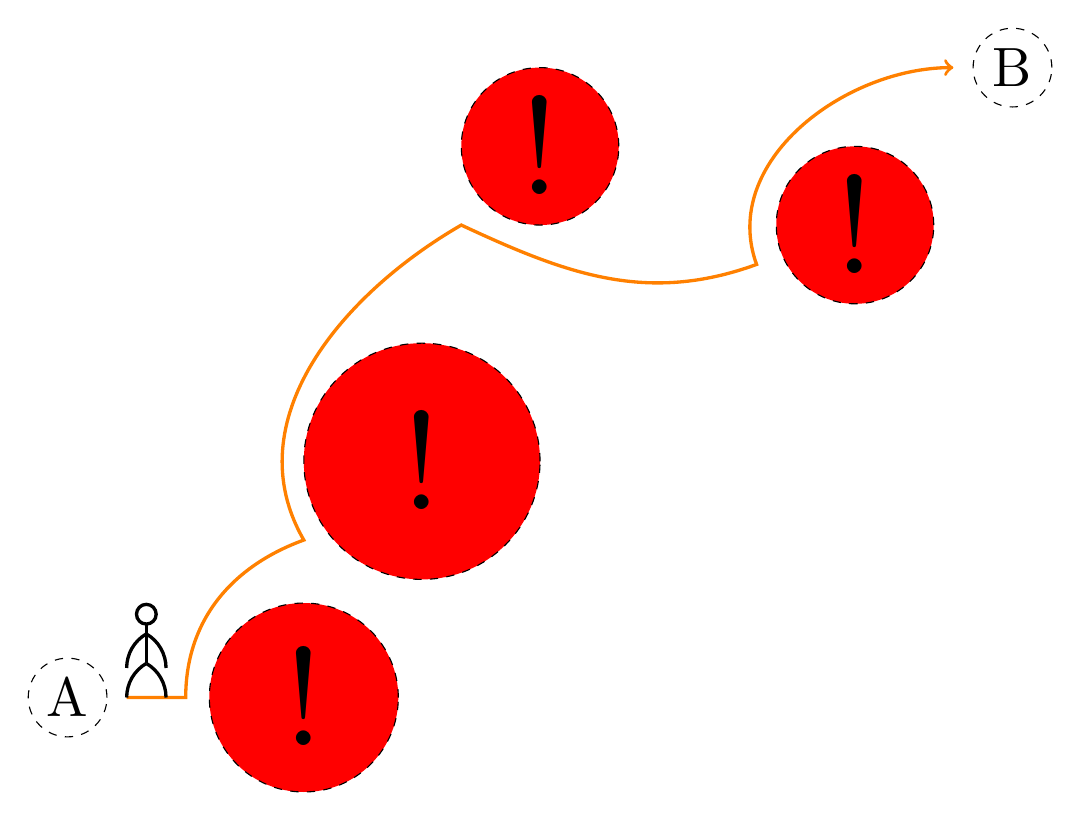
\begin{tikzpicture}
			\draw [dashed] (0,0) circle [radius=0.5];
			\draw (0,0) node[scale=2]{A};
			
			\draw [dashed] (12,8) circle [radius=0.5];
			\draw (12,8) node[scale=2]{B};
			
			\draw [dashed, fill=red] (3,0) circle [radius=1.2];
			\draw (3,0) node[scale=5]{!};
			
			\draw [dashed, fill=red] (4.5,3) circle [radius=1.5];
			\draw (4.5,3) node[scale=5]{!};
			
			\draw [dashed, fill=red] (6,7) circle [radius=1];
			\draw (6,7) node[scale=5]{!};
			
			\draw [dashed, fill=red] (10,6) circle [radius=1];
			\draw (10,6) node[scale=5]{!};
			
			\draw [->,very thick, orange] (0.75,0) to [out=0,in=180] (1.5,0) to [out=90,in=200] (3,2) to [out=120,in=-150] (5,6) to [out=-25, in=-160] (8.75,5.5) to [out=110, in=180] (11.25,8);
			
			\draw [very thick] (1,0.433) arc [radius=0.5, start angle=120, end angle=180];
			\draw [very thick] (1,0.433) arc [radius=0.5, start angle=60, end angle=0];
			\draw [very thick] (1,0.433) -- (1,0.933);
			\draw [very thick, fill=white] (1,0.433+0.625) circle [radius=0.125];
			\draw [very thick] (1,0.433+0.375) arc [radius=0.5, start angle=60, end angle=0];
			\draw [very thick] (1,0.433+0.375) arc [radius=0.5, start angle=120, end angle=180];
		\end{tikzpicture}
		
		\caption{Unknown dangerous environment}{This image illustrates an environment, observed from above, in which a human must move from point \emph{A} to point \emph{B} while avoiding invisible dangerous areas. \emph{A} is the start location, \emph{B} is the goal ant the red circles represent dangerous zones. We provide in this thesis a solution to guarantee safeness in such circumstances. Possible applications for this type of solutions are: mine fields crossing and cleaning, radioactive areas avoidance,...}
		\label{fig:unknown_environment}
	\end{figure}
	
	
	\section{Solution}
	
	\begin{comment}
	[Solution at high level and the problems I will have to solve? Faire le lien avec flocking et pattern. \textcolor{red}{The swarm is extending the perception capabilities of the human.} Challenges.
	On a choisit d'utiliser des swarms car... Equidistance par rapport à l'humain. Carac du système. Pb pour détecter l'humain...avec solution. Agent de la swarm doit être capable de détecter le danger. Humain perçoit la swarm qui elle perçoit le danger.]
	\end{comment}
	
	The solution we propose involves the use of a swarm of robots. Swarm robotics systems are well suited for this types of application because it is compatible with unknown environments thanks to its flexible, robust and scalable characteristics \citep{brambilla2013swarm}. In case of failure of one or a few robots, the system would continue to provide sufficient performance thanks to its scalability and robustness.
	
	In our solution, a swarm of robots forms a round shield around a user (i.e., they form a circle around the user). The round shield formed by the swarm enables a 360° protection of a user. All the robots try to stay at the same distance from each other and the human. However, when a danger is detected, the robots might not respect that rule to form a boundary on the edge of the danger zone. To achieve this, the solution relies on the pattern formation theory widely used in swarm robotics. The corresponding techniques will be explained in the next chapter with more details. If the number of robots is not high enough to form a complete circle, an arc is formed at the front to always shield the most critical zone.
	
	As shown on Figure \ref{fig:swarm_preventing}, the robots in contact with a dangerous zone will report the danger through visual communication with the human. Here the robots light on their orange LEDs and stay on the boundary of the zone to prevent the human from getting into it. Since the human cannot see the danger, and only the robots can, we can see that the swarm is increasing the perception capabilities of the human.
		
	\begin{figure}[!htp]\centering
		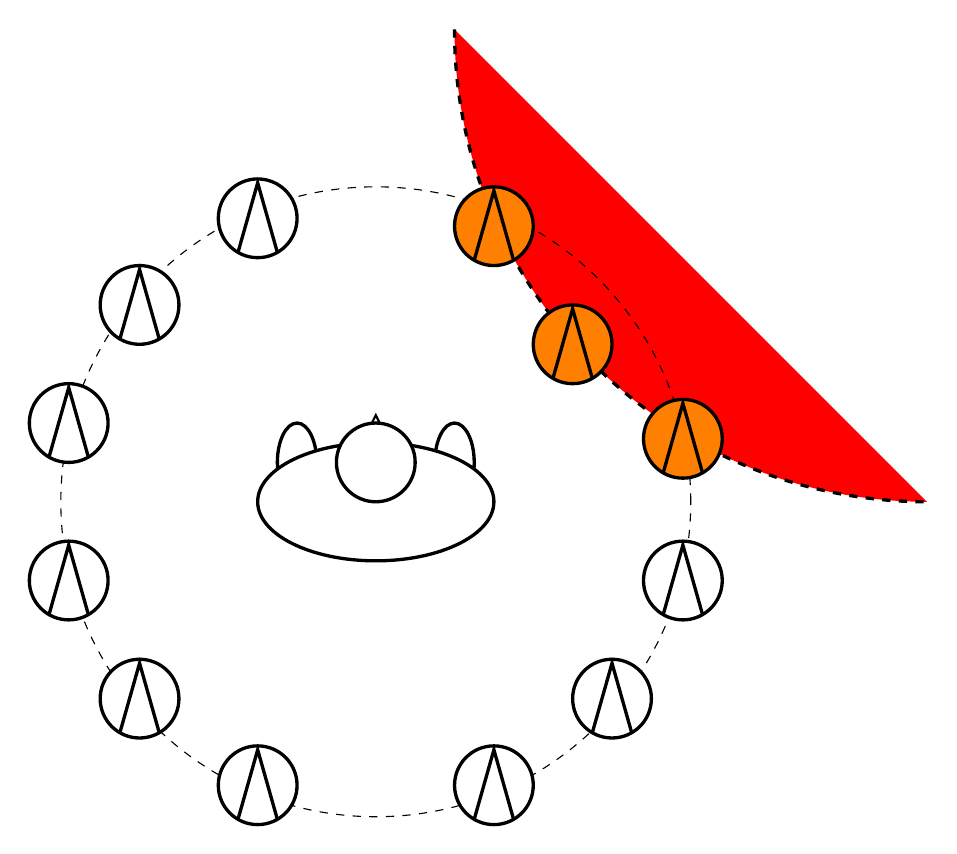
\begin{tikzpicture}
		
		%	\foreach \i in {\xMin,...,\xMax} {
		%        \draw [very thin,gray] (\i,\yMin) -- (\i,\yMax)  node [below] at (\i,\yMin) {$\i$};
		%    }
		%    \foreach \i in {\yMin,...,\yMax} {
		%        \draw [very thin,gray] (\xMin,\i) -- (\xMax,\i) node [left] at (\xMin,\i) {$\i$};
		%    }
			
			\draw [very thick, dashed, fill=red] (2,6) arc [radius=6, start angle=180, end angle=270];
			
			\human{1}{0}
			
			\draw [dashed] (1,0) circle [radius=4];
			
			\epuckred{2.5}{3.5}
			\epuckred{3.5}{2}
			\epuckred{4.9}{0.8}
			\epuck{4.9}{-1}
			\epuck{4}{-2.5}
			\epuck{2.5}{-3.6}
			\epuck{-2.9}{-1}
			\epuck{-2}{-2.5}
			\epuck{-0.5}{-3.6}
			\epuck{-2.9}{1}
			\epuck{-2}{2.5}
			\epuck{-0.5}{3.6}
					
		\end{tikzpicture}
		
		\caption{Swarm prevention}{This figure is a symbolic representation of a human helped by a swarm. The circles with a triangle inside are representations of a robot. The swarm tells the human that a dangerous zone is located at the front right by visual communication (here the robots change their colour to red). The swarm stays at the boundary to form a \enquote{shield}. The direction taken by each individual in the swarm is given by the triangle inside (here heading north).}
		\label{fig:swarm_preventing}
	\end{figure}
	
	One issue that had to be resolved was the detection of the human by the robots. As \citet{podevijn2012self} suggested, the interface between the human and the robots swarm should be restricted to the strict minimum because in the field the infrastructure needed to operate the swarm might not be easy to build and manipulate. The swarm should handle the communication on its own. As a big infrastructure such as a tracking system, or any interface of the same kind would have been difficult to use in real life applications, we designed and implemented a compact, wearable device that allows a human to be recognised by the robots: a pair of shoes.
	
	Figure \ref{fig:shoes} illustrates the use of the shoes (no user is wearing them to not occlude the field of view). In Figure \ref{fig:shoes} (left), the robots have just recognised the shoes thanks to the LED system inside and begin to move in order to form a circle around the shoe. On Figure \ref{fig:shoes} (right), we show an example of one configuration obtained after 3 minutes, viewed from above.
	
	\begin{figure}[!htp]
		\begin{minipage}[c]{0.6\textwidth}
			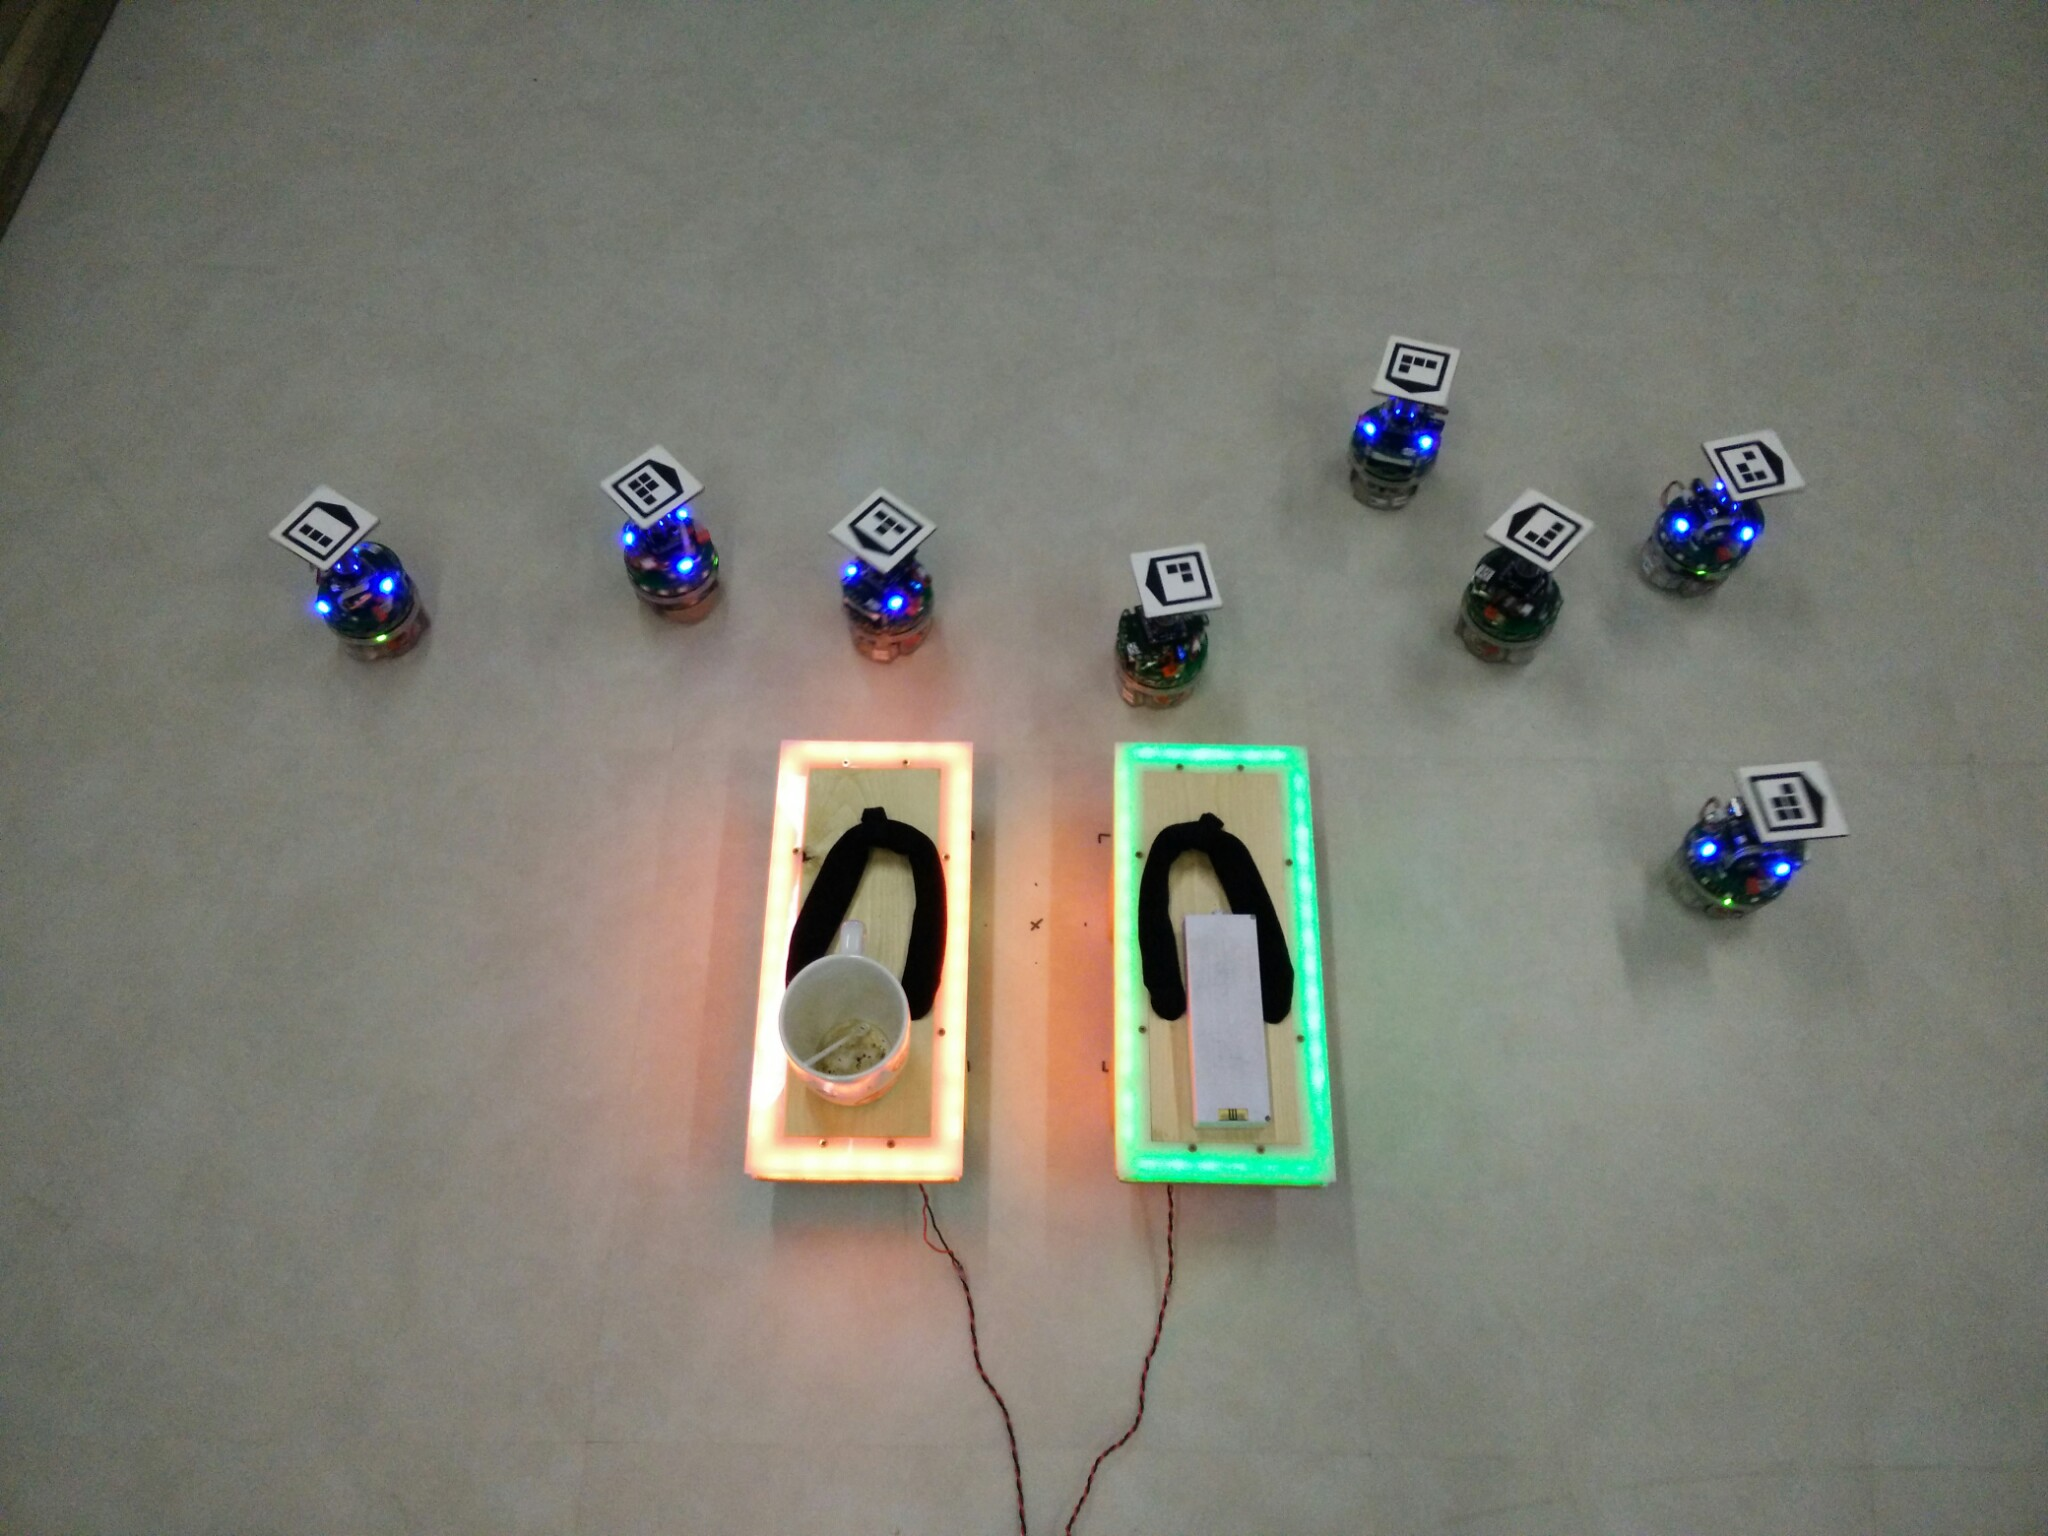
\includegraphics[trim=200px 300px 140px 300px, clip=true, height=5cm]{images/shoes.jpg}
		\end{minipage}
		\hfill
		\begin{minipage}[c]{0.39\textwidth}
			\hfill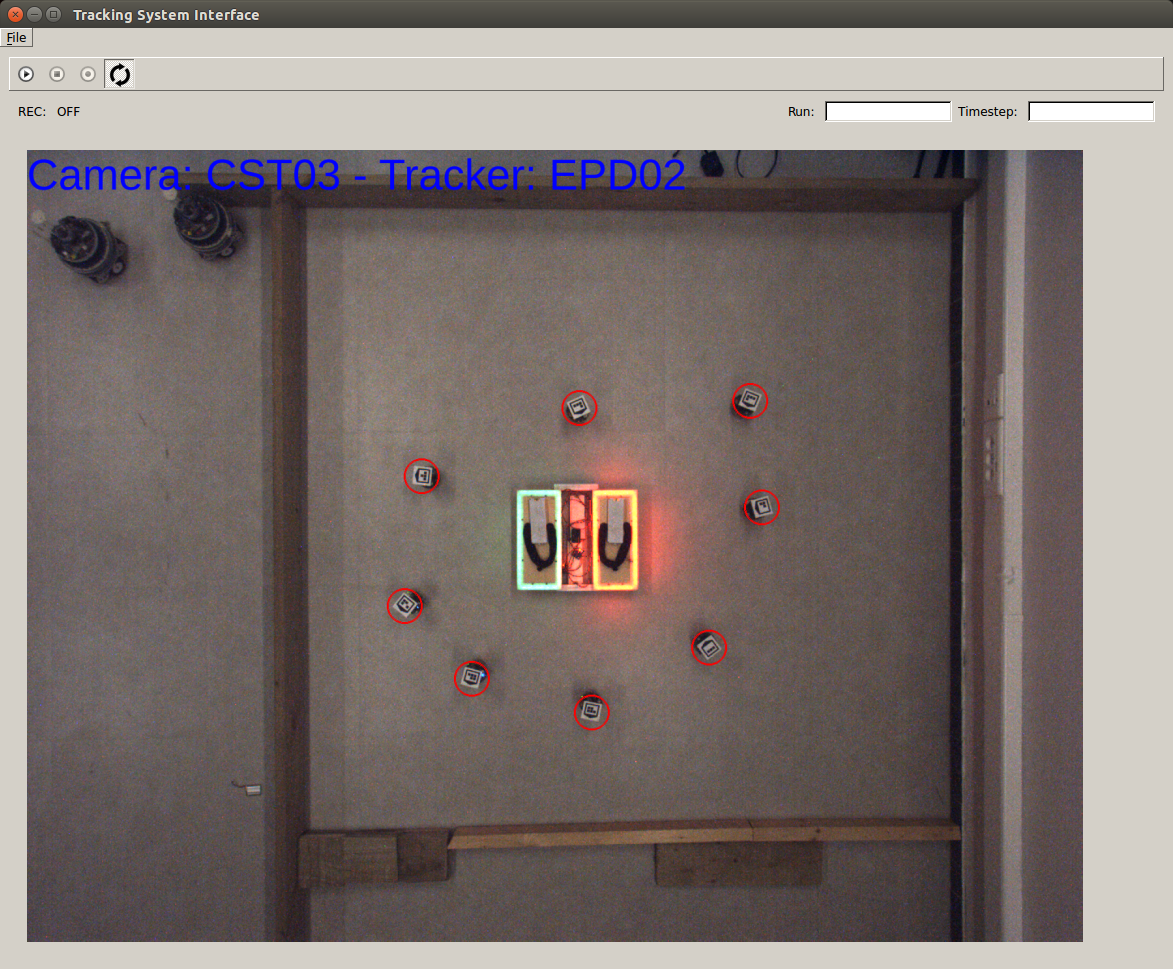
\includegraphics[trim=380px 230px 380px 360px, clip=true, height=5cm]{../Experiments/No_Human/6end.png}
		\end{minipage}				
		
		\caption{The shoes}{This picture shows a prototype of the shoes viewed from above, and the robots interacting with the shoes. The interaction is enabled through the recognition of the colours, one for each shoe, indicating left (red) or right (green) side. This pair of shoes enables the robots to locate the user, allowing them to evolve at the target distance from him/her. On the left image, the robots are still in the process of placing themselves in a correct circle. The right image depicts the situation after a 3 minutes experiment where the robots were initially placed in lines around the shoes. Objects are put on the shoes to close the lights switch (normally activated by the weight of the user).}
		\label{fig:shoes}
	\end{figure}

Our objective in this thesis, is to present an innovative protection using swarm robotics. The results obtained from experiments with a swarm of real robots are presented in the chapter \ref{chap:experiments}.

\section{Implementation}

	In this section, we present the solution to the problem described in section \ref{sec:the_problem} and all the choices that resulted in it. The explanation will follow a top-down approach. We first review the hardware and the code architecture. Then, we will detail our implementation.
	
	We decided on swarm robotics because, as stated in section \ref{def:robustness_scalability_flexibility}, robustness, scalability and flexibility are characteristics that make swarm robotics systems well suited for unknown environments \citep{brambilla2013swarm}. In case one of the agents is broken, we do not want to see the whole system collapse and leave the human unattended. The solution guarantees that the solution will work in different conditions, environments, which is an advantage for exploration and rescue (flexibility). In case of loss of robots, scalability would maintain the protection performance to an acceptable level.
	
	\subsection{The Hardware}
	
	In the following section, we present the robotic platform used in our experiments, and the device allowing the robots to detect the human.
	
		\subsubsection{E-puck}
		\label{sec:e-puck}
		
		The robotic platform chosen was the e-puck \citep{mondada2009puck} because the laboratory possess approximately 28 of them, along with the appropriate modules (omnidirectional camera, top LEDs). Furthermore, the academic personnel had developed a good knowledge of the platform. The e-puck robot platform was made for educational purposes. Its shape is cylindrical with a diameter of 7.5 cm. It is moved by two diametrically opposed wheels. Figure \ref{fig:e-puck_red_zones} (left) shows an e-puck from the laboratory. Several extensions (modules) were plugged onto it to increase its capabilities. In this thesis, in the final solution, we used the proximity sensors, the omnidirectional camera sensor and the virtual ground sensor. The proximity sensor is made up by 8 infrared sensors. Each infrared sensor returns a value proportional to the proximity of a nearby obstacle in the $[0,1]$ interval. The infrared sensors are placed along the perimeter of the robot. The omnidirectional camera is a vertical camera placed on the top of the e-puck's base, aiming at a convex mirror to provide a 360° view of the environment. It translates this view into a list of colour blobs. A colour blob is a cluster of pixels being almost of the same colour. During the calibration, among other parameters, one can tune the degree of similarity, the minimum size of the cluster, and the recognised colours. The last sensor is different: it is not real, and not physically present on the board \citep{reinaaugmented}. It is simulated through the ARGoS simulator used to develop the controller of the robot \citep{pinciroli2012argos,GarFraBruPinBir2015:techreport-004}. It sends data created inside the simulator to the robot, from the simulated environment. In our case, this data contains the colour of the ground, symbolising the presence of danger. We actually simulated red discs on the floor through the simulator to artificially set up dangerous areas that were not visible by the testing user. That way, the conditions of real life application were the closest possible to ours. An example of red zone is in Figure \ref{fig:e-puck_red_zones} (right). The positions of the robots inside the simulator are determined by the use of a tracking system \citep{stranieri2013iridia}. The virtual positions correspond to the real positions. Using a virtual sensor enables early experimentation by removing the need to implement a real sensor. The real robots actually have a ground sensor. However, as during the tests the human cannot see the dangerous zones, we could not use any visible colour. A new type of ground sensors, able to detect other types of information was necessary. Hence we chose to create a ground virtual sensor that detects colours that are only present in the simulator, not physically present in the laboratory. That way, the dangers remain invisible to the human doing the experiments, but visible by other operators watching the simulator screen.
		
		\begin{figure}[!htp]
			\begin{minipage}[c]{0.49\textwidth}
				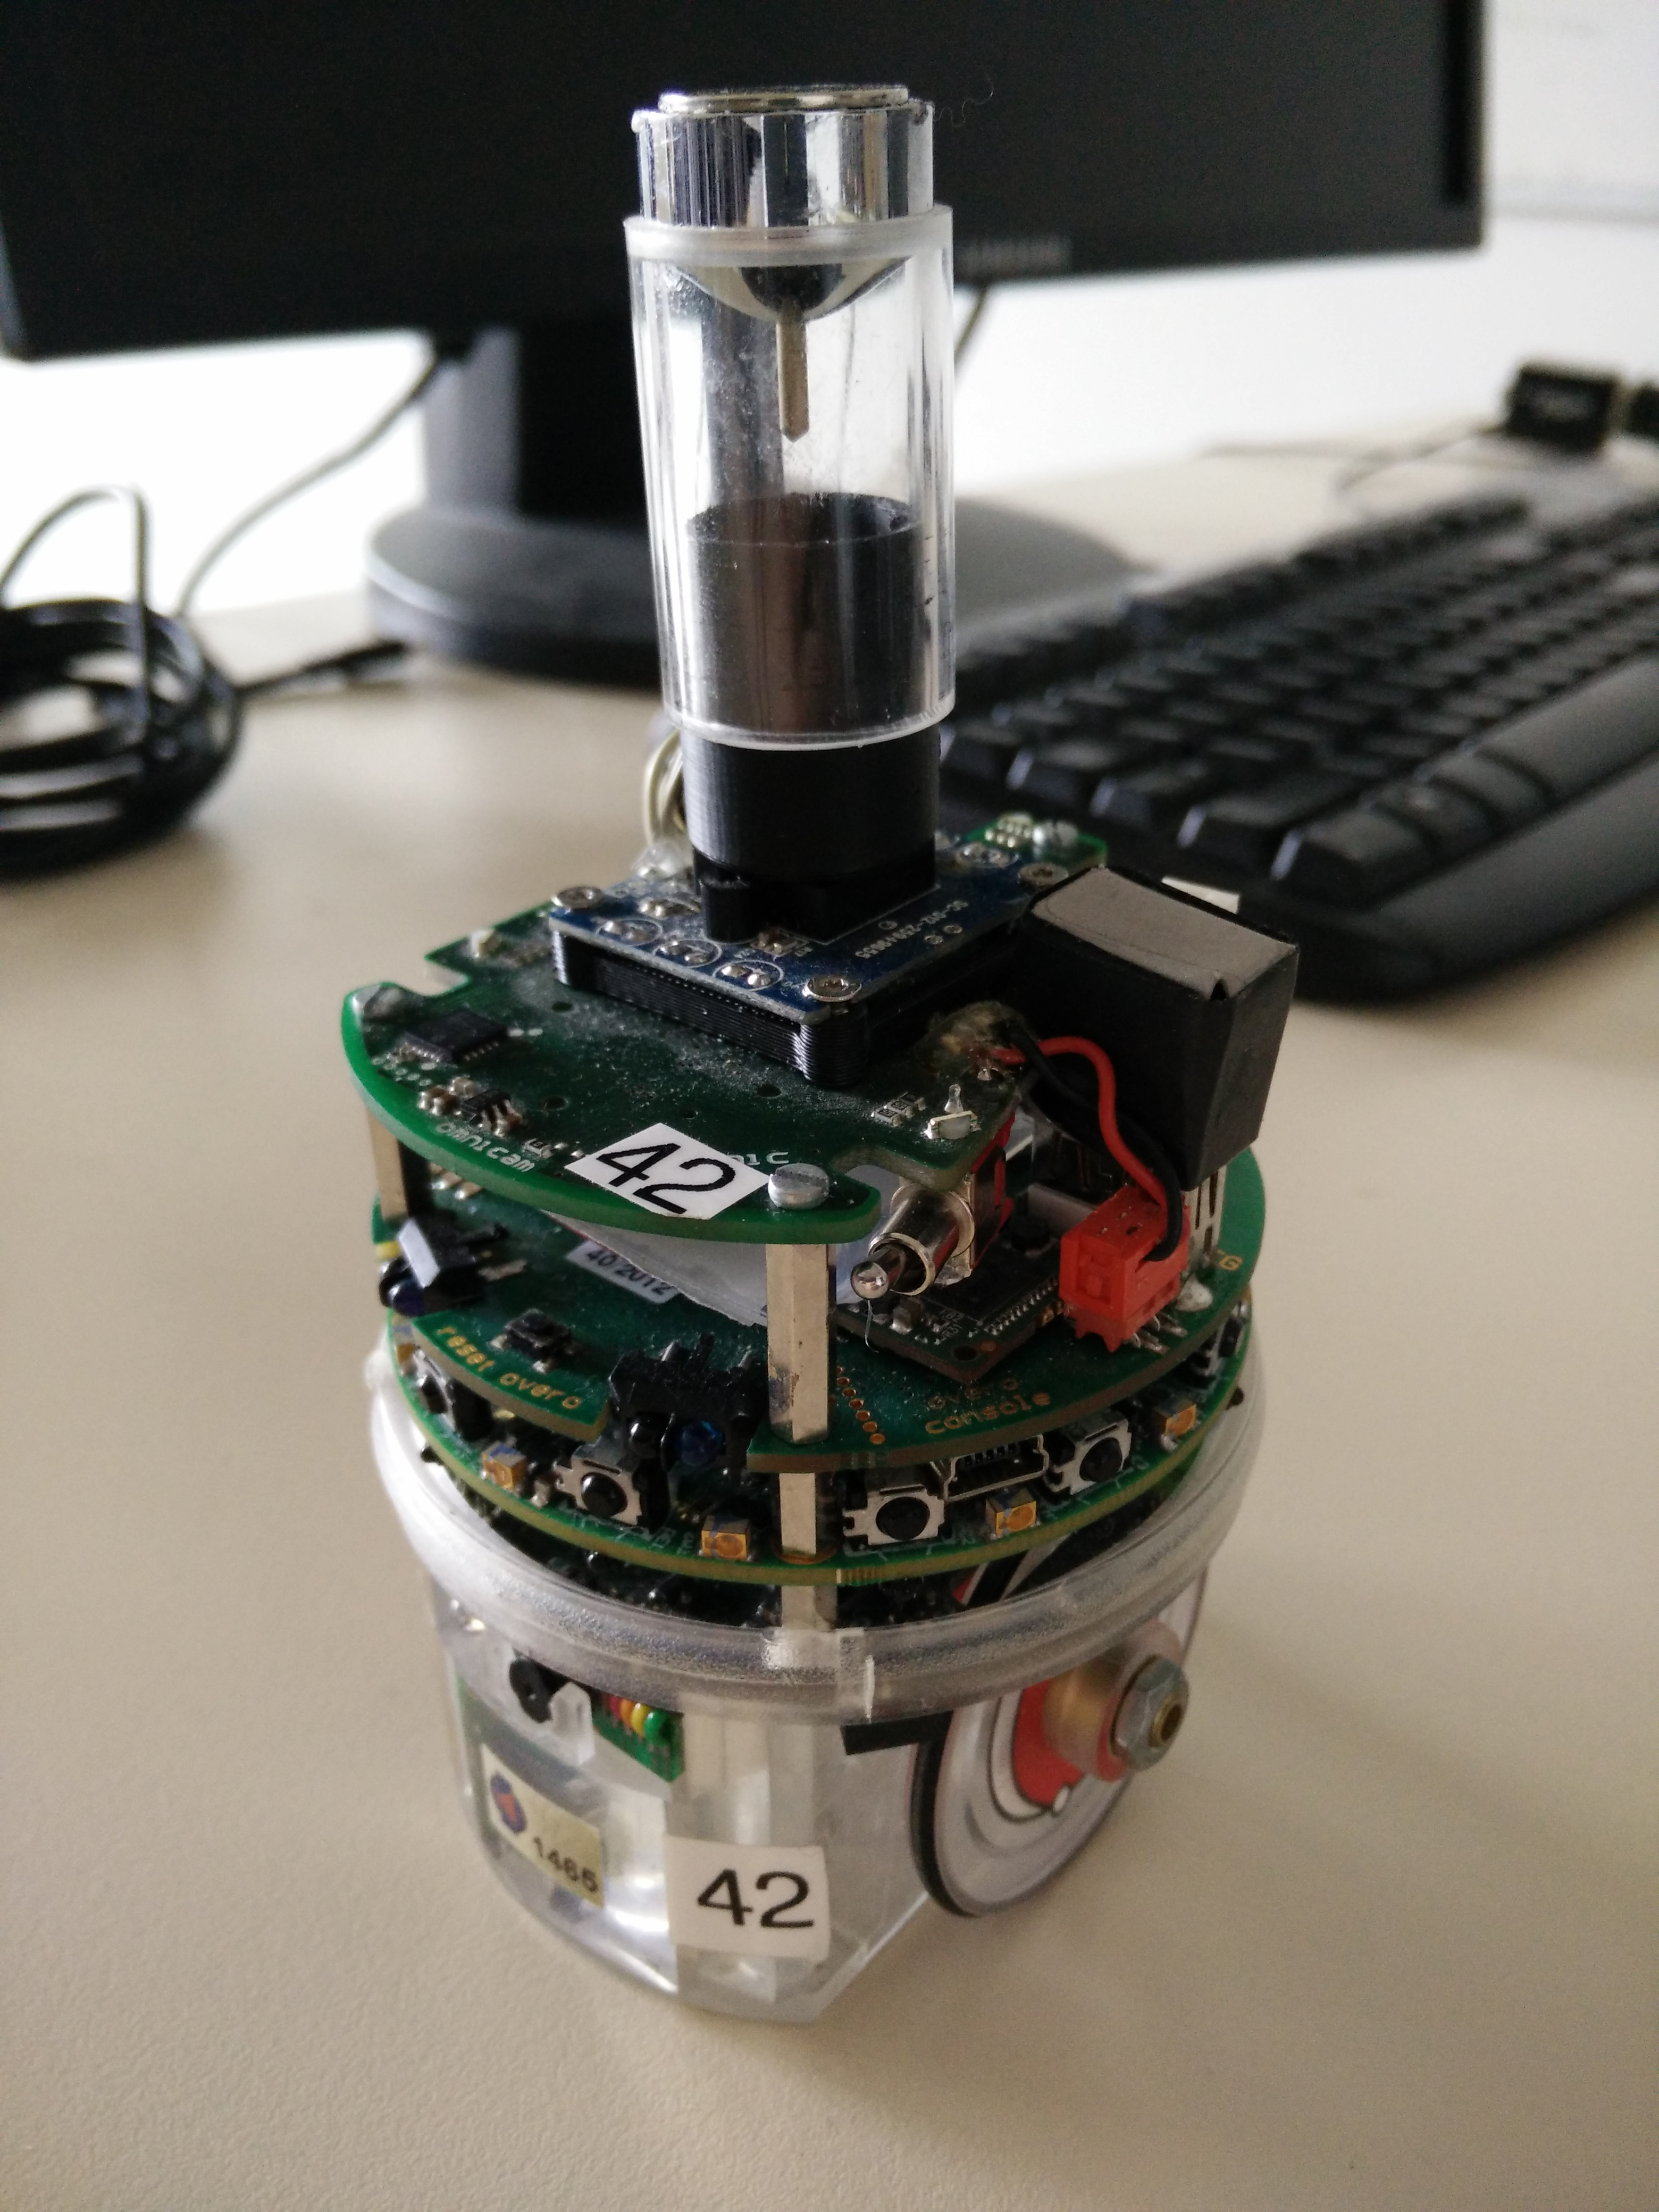
\includegraphics[height=7cm]{images/e-puck.jpg}			
			\end{minipage}
			\begin{minipage}[c]{0.49\textwidth}
				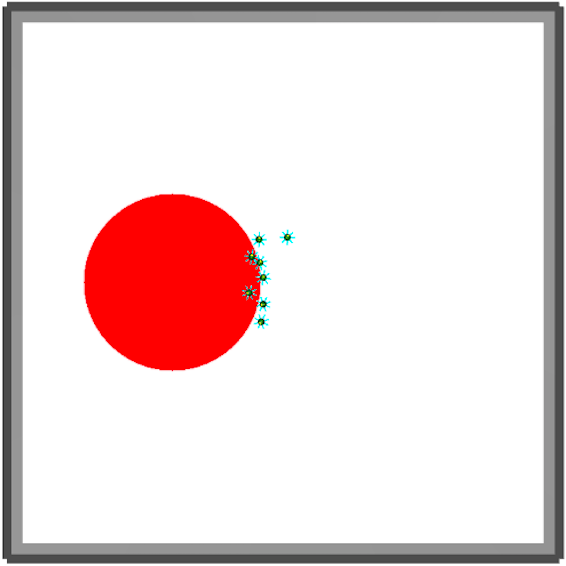
\includegraphics[width=\textwidth]{../Experiments/No_Human/red_circle.png}			
			\end{minipage}
			
			\caption{The E-puck and its virtual sensor}{On the left, one can see a picture of the robotic platform we used: the E-puck. Our swarm is composed of several robot like this one. On the right is a screen capture of the ARGoS simulator \citep{pinciroli2012argos} where the danger virtual sensor is used. Virtual means that it is not real, not physically present on the board. It is simulated through the ARGoS simulator. It sends data created inside the simulator to the robot, from the simulated environment. It augments the robot sensing capabilities. In our case, this data contains the colour of the ground, symbolising the presence of danger. The red circle represents a danger zone in which no human can go. No human can see it though. The small dots are representations of the real robots inside the simulator.}
			\label{fig:e-puck_red_zones}
		\end{figure}
		
		\begin{comment}
		[4ème capteur essayé, sur papier avait plus de potentiel car moins contraignant, mais comportement complètement imprévisible, calibration impossible, passé sur l'OC]
		\end{comment}
		Before considering the omnidirectional camera as the best option, another sensor was examined: the range and bearing sensor \citep{gutierrez2009open}. The range and bearing extension is a infrared communication board that also provides the range (distance) and the bearing (angle) of the emission source. On paper it seemed like a better option because it was less restrictive than the omnidirectional camera. With the camera, a precise calibration of the different colours is required to avoid errors. The range and bearing uses a CRC code to detect errors in the data received, thus ensuring the correct recognition of the different entity types in the environment. The number of different entities (colours) is very limited with the omnidirectional camera as a result of the algorithm behind it. The range and bearing actuator can send up to 4 bytes of data, multiplying the amount of different entities (one string of bits for each entity). It is also less sensitive to light conditions. Unfortunately, after multiple attempts to use the range and bearing, we realised that it was unusable. It behaves in a completely unpredictable way with the range value. We tried to calibrate it, but to no avail. Figure \ref{fig:rab_intensities} illustrates the wide distribution of message intensities causing an imprecise measure of the range (distance of the source). This figure is only for one run of the experiment. Consecutive runs yielded very different results for the same experiment configuration.
		
		\begin{figure}[!htp]
			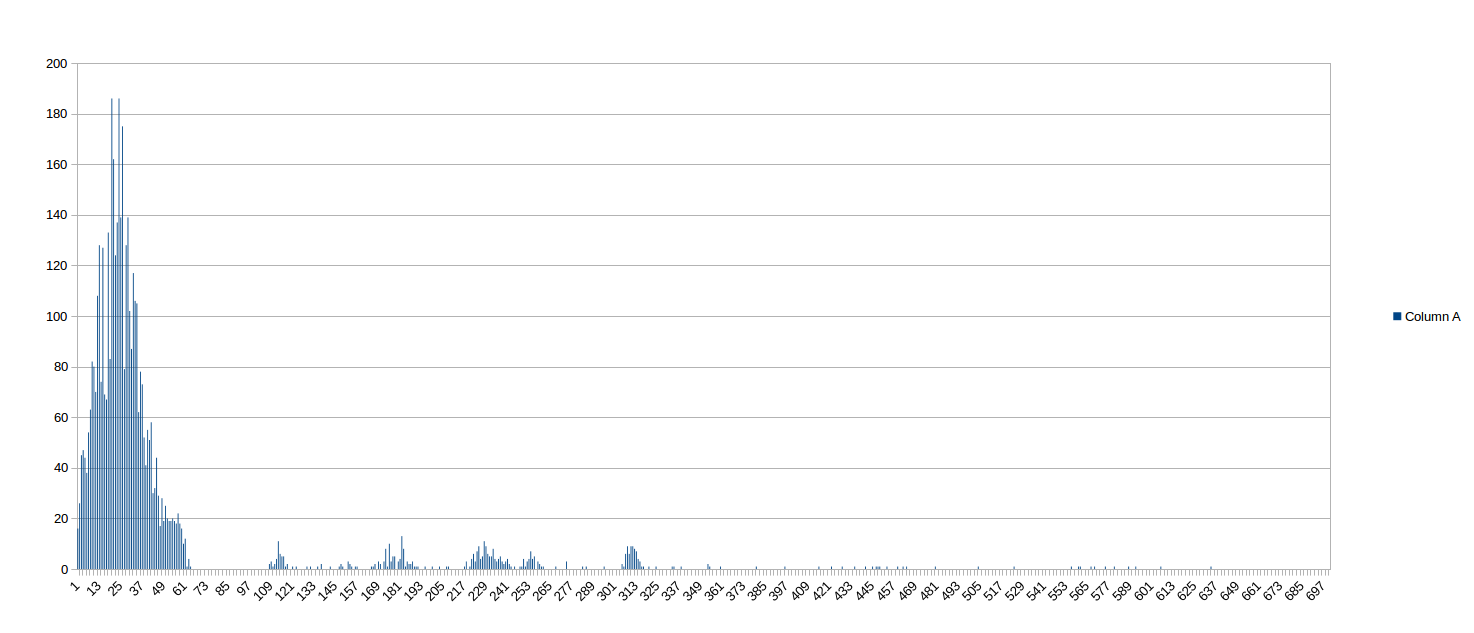
\includegraphics[trim=35px 0px 100px 0px, clip=true, width=\textwidth]{images/powers_29-28.png}
			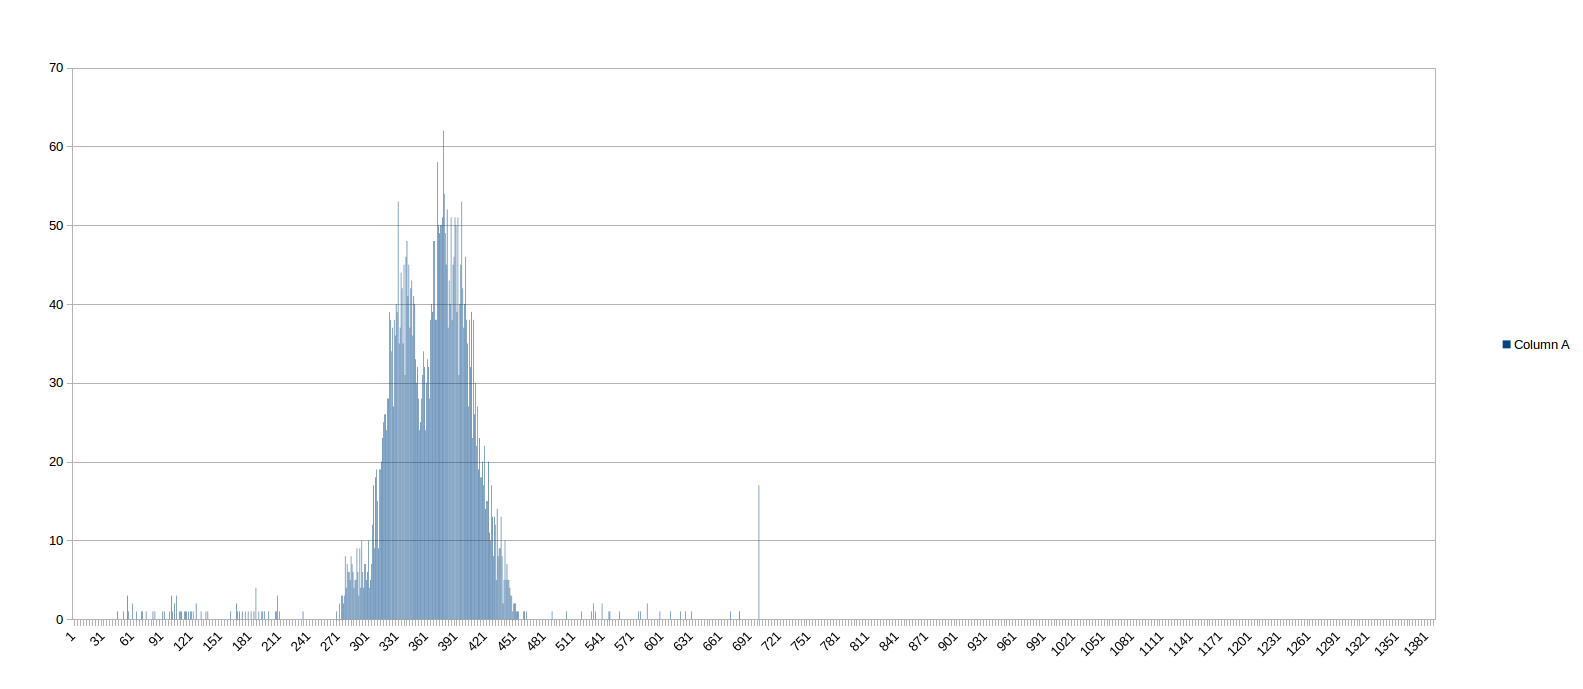
\includegraphics[trim=35px 20px 100px 0px, clip=true, width=\textwidth]{images/powers_54-28.png}
			\caption{Intensities of the RAB messages}{This figure shows the absolute frequencies of the range and bearing messages intensities for a duration of 3 minutes. During these 3 minutes, one robot is emitting messages and rotating on itself. Another robot is placed at 25 centimetres of the first one and receives the messages. The message intensity can vary from 0 to 1023 on the x axis. The y axis is the absolute frequency. Each graph corresponds to a different emitting robot. On the upper graph, one can see that frequency pikes can appear far away from the \enquote{normal} average value. On the lower graph, the interval of intensity is very big. Other runs of the experiment with the same robots yielded very different results. The current implementation of the RAB sensor is thus a bad choice for the measure of the distance between robots.}
			\label{fig:rab_intensities}
		\end{figure}
		
		\paragraph{Limitations}
		
		Although the omnidirectional camera worked better than the range and bearing, it was still restrictive. The difficulty of the calibration, and the error rate, increase with the amount of recognised colours. We limited ourselves to 3 colours: red, green and blue. Another limitation was the speed of the robot, limited to 10 cm/s. Normal speed for a human walking is about 5 km/h or 140 cm/s \citep{wiki:002}. In these circumstances we had to reduce the walking speed of the user during the demonstration and the tests. The battery was also an issue. The autonomy of one robot is between 30 minutes and one hour when moving a lot. Changing batteries and restarting the robots multiple times was necessary during long testing sessions. Since the robot only has two wheels, it maintains its equilibrium by lowering the chassis. The front or the back of the robot always touches the ground, making it impossible to use on uneven grounds. The floor of the arena, the room where all the experiments were done, is composed of adjacent squares. Sometimes the robots would get stuck between two squares. Moreover, the activity LEDs on the different circuit boards composing the robots interfered with the omnidirectional camera, taking them as other robots. We had to cover them with pieces of tape, and change the calibration to not take into account the blobs that were too small.
		
		\subsubsection{E-geta} % Longer text than for e-puck because more important!
		\begin{comment}
		[I will in this section describe the need for a device to detect a human and its development. What are the objectives of the hardware? The choices we made to get the final solution. How we built it. Calibration an adaptation process to make the current algorithm compatible with the new hardware. Where does the term come from?]
		\end{comment}
		
	As explained in chapter \ref{chap:escorting_swarm}, one of the main issue was to enhance the robots so they could detect the user and position themselves with respect to him without any large external equipment. Large external equipments are not recommended since, in the targeted unknown environment, they might not be usable. For example, one might use a tracking system to get the position of the robots in real time and communicate it to the robots for them to adjust their speed. In a controlled environment, this may work very well, but in the field it would be difficult to deploy such a tracking system.
	
	We thus opted for a compact, wearable device that would act as a \enquote{landmark} for the robots: a pair of shoes. In order for the robots to understand on which side of the human they are (to go in front of him/her), the two shoes have to emit a different message. The two shoes have to emit a different colour to give the robot information on the direction of the human. In section \ref{sec:robot_behaviour} we come back on the algorithm used to deduce the direction of the human from the observed colours.
	
	\begin{comment}
	[Inspiration des getas. Plan ou modèle 3D. Méthode de construction (laser cut pour les plexi etc). Circuit électronique.]
	\end{comment}
	
	\begin{figure}[!htp]
		\begin{minipage}[c]{0.49\textwidth}
			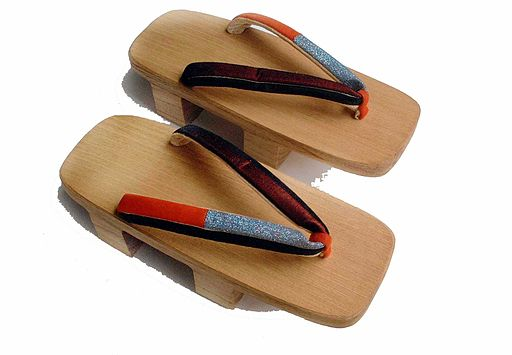
\includegraphics[width=\textwidth]{images/512px-Geta.jpg}
		\end{minipage}
		\hfill
		\begin{minipage}[c]{0.49\textwidth}
			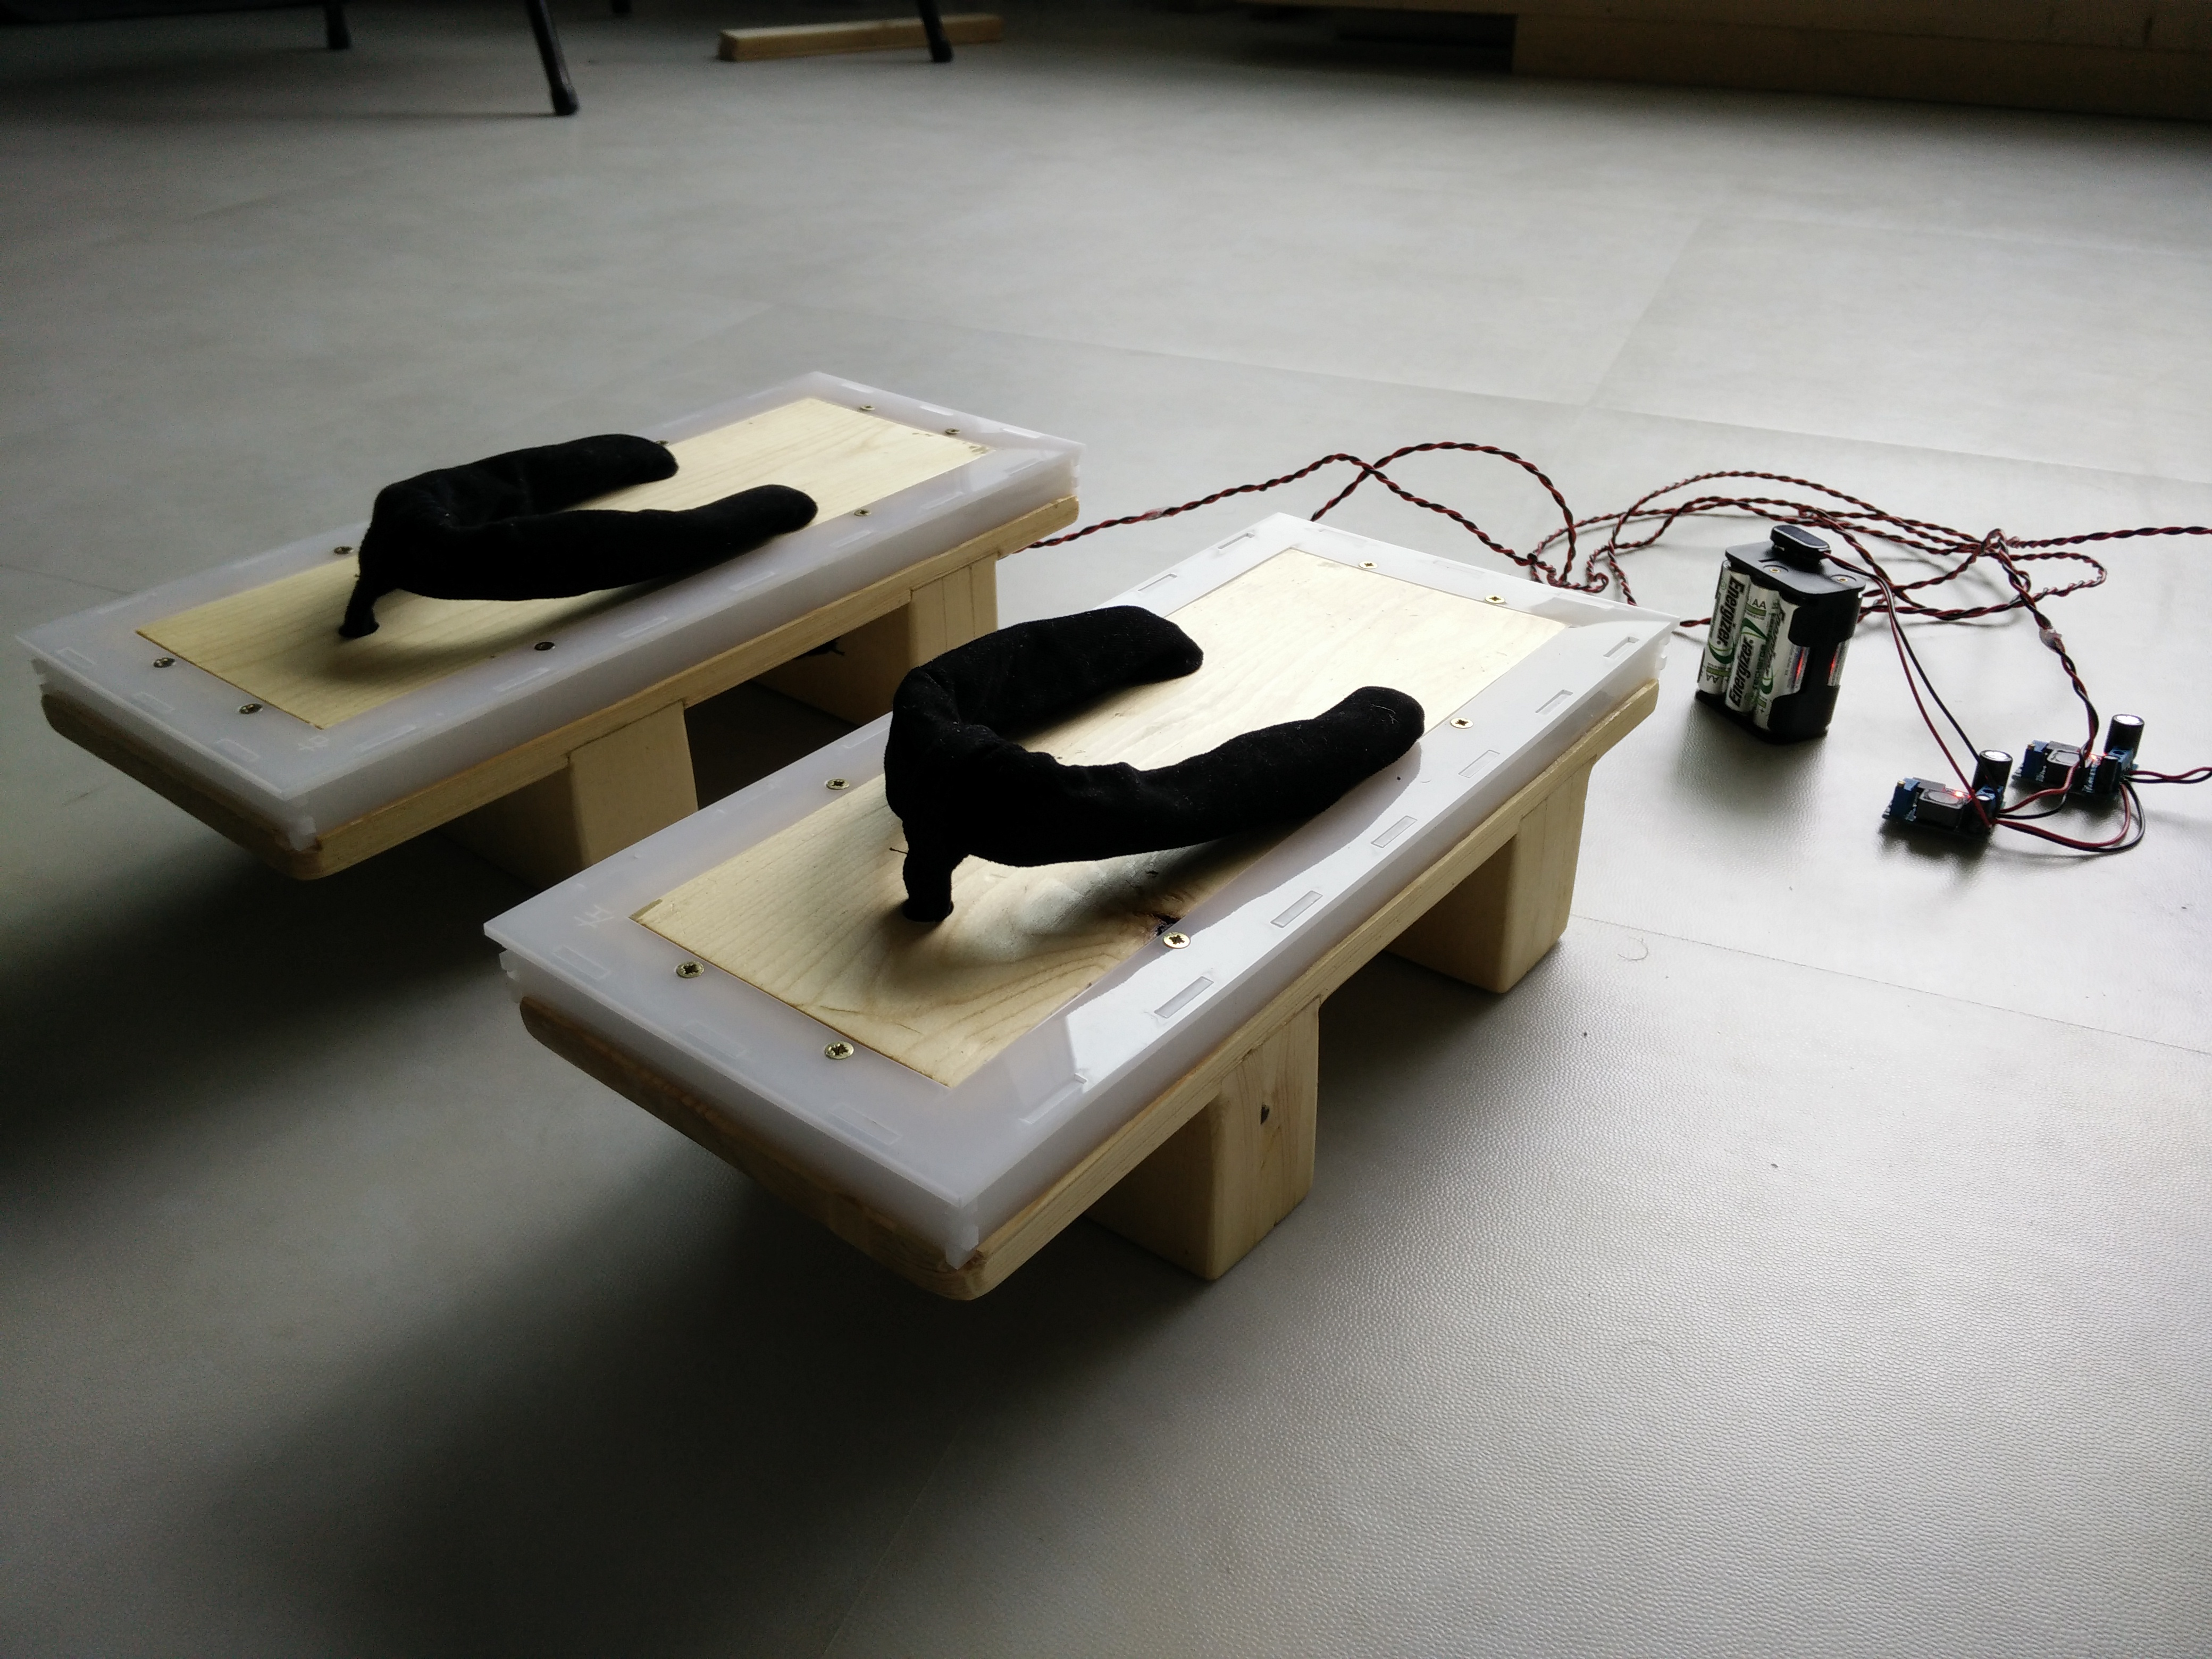
\includegraphics[width=\textwidth]{images/shoes2.jpg}
		\end{minipage}
		
		\caption{E-Geta}{Left image by Haragayato [GFDL (http://www.gnu.org/copyleft/fdl.html) or CC-BY-SA-3.0 (http://creativecommons.org/licenses/by-sa/3.0/)], via Wikimedia Commons. Found on \citet{wiki:001}. On the right is a picture of our prototype shoes, connected to their battery through voltage regulators. See Figure \ref{fig:circuit} for the circuit.}
		\label{fig:e-geta}
	\end{figure}
	
	We took inspiration from the Japanese \enquote{geta} shoes for the design. Figure \ref{fig:e-geta} shows a picture of a Japanese wooden shoe called geta. The right side of the figure is a picture of our prototype. The two have the same overall design. We chose this design in order to slow down the human's speed. Indeed, the speed of the robots is limited to maximum 10 cm/s per wheel. Another advantage is the simplicity of the structure, and the low number of assembly parts.
	
	The base of the shoe is made with wood. The surrounding piece covering the LEDs was cut in sheets of semi-opaque plexiglass to diffuse the light. The LEDs are standard strip LEDs (one red strip, and one green). The electronic circuit (Figure \ref{fig:circuit}) is made up by a 9 volt battery connected to two variable voltage regulators. The two regulators are step up in parallel in order to increase the potential on the output. Each regulator is connected to a shoe LED strip. A separation is necessary since the green LED strip requires more energy than the red one. To get an equivalent luminosity for both shoes, a different voltage had to be applied.
	
	\begin{figure}[!htp]\centering
		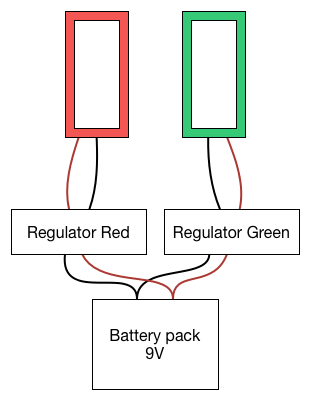
\includegraphics[scale=0.5]{figures/circuit.png}
		\caption{The circuit}{The figure shows a sketch of the final electronic circuit for the shoes. The battery delivers 9 volts to two regulators in parallel, one for each shoe since each one of them need a different energy supply. Indeed, the green LED strip is more power hungry than the red one. The mass (black cable) is common for all the circuit.}
		\label{fig:circuit}
	\end{figure}
	
	\subsection{The Robot Behaviour}
	\label{sec:robot_behaviour}
	
	\begin{comment}
		Pour parvenir à mes fins, j'ai dû implémenter un controller. J'ai choisi virtual physics car ces avantages et inconvénients. C'est ce gars qui l'a inventé, et voici les travaux utilisant cette technique.
		0) Aspect solution avec cercle.
		1) Dois faire un controller en c++, pour la plateforme ARGoS, mais aussi compatible e-puck.
		2) Design de la state machine.
		3) Virtual physics. Les forces pour chaque state, l'idée de l'algorithme derrière, et leur évolution.
		4) Les paramètres les plus importants ? Le fait qu'on peut les changer.
		5) Comment traduire le vecteur de direction en vitesse de roue.
	\end{comment}
	
	The first step of the design of the solution is to imagine how the system will look like and how we will implement it (how do the robots move around the human, what shape will they try to form). This part is important because it will define the overall look and performance of the system.
	
	We decided on a circle shape because it is the easiest to realise in practice in the pattern formation theory. It offers the best ratio
	$$\frac{\mbox{\textit{Surface}}}{\mbox{\textit{Perimeter}}} = \frac{\pi r^2}{2\pi r} = \frac{r}{2}~\mbox{,}$$
	 where $r$ is the radius of the circle. That means that fewer robots are needed for the same protected area, and more space for the human with a certain amount of robots than any other possible shape. The Figure \ref{fig:circle_shape} represents the kind of circle that we would like to obtain for 6 robots and 1 human in the centre.% All the robots are equally distanced from each other and the human. The human is protected in all directions. In presence of danger, the robots in contact with it should report it to the human and prevent him from going towards it, as seen on Figure \ref{fig:swarm_preventing}. In that case, the conditions concerning the target distance from the human and between robot may not be respected.
	
	\begin{figure}[!htp]\centering
	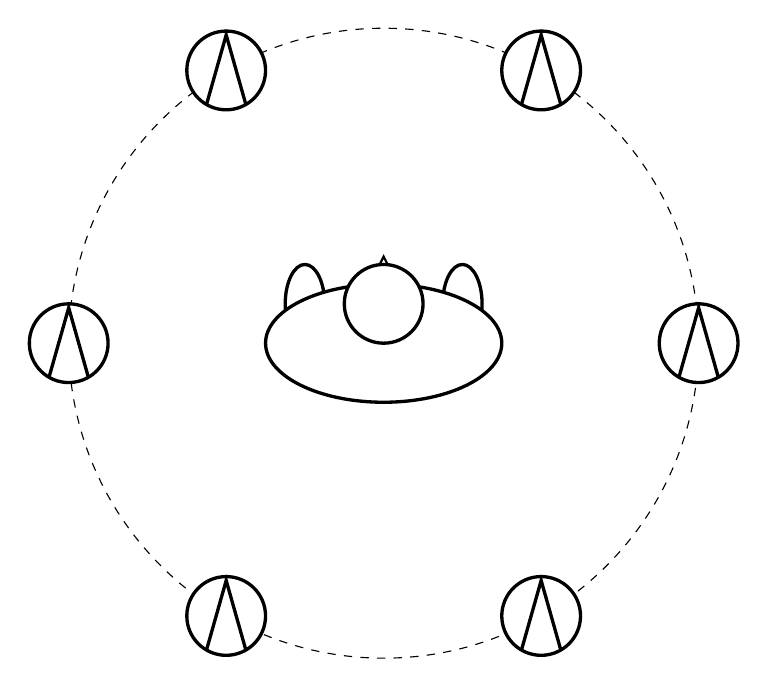
\begin{tikzpicture}
		\draw [dashed] (0,0) circle [radius=4];
		\epuck{4}{0}
		\epuck{2}{3.464}
		\epuck{-2}{3.464}
		\epuck{-4}{0}
		\epuck{-2}{-3.464}
		\epuck{2}{-3.464}
		
		\human{0}{0}
	\end{tikzpicture}
	\caption{Ideal behaviour in absence of danger}{This figure symbolises the ideal behaviour required in absence of danger. The swarm forms a circle to cover the widest protected surface for a given amount of robots. All the robots are equally distanced from each other and the human. The human is protected in all directions. In presence of danger, the robots in contact with it should report it to the human and prevent him from going towards it, as seen on Figure \ref{fig:swarm_preventing}. In that case, the conditions concerning the target distance from the human and between robot may not be respected.}
	\label{fig:circle_shape}
	\end{figure}	
	
	Implementing a robots swarm behaviour means writing a controller code for its individual components: the robots. The laboratory provides a template for this purpose. The logic of the individual behaviour is added inside callback methods called either by the simulator when performing simulations inside ARGoS \citep{pinciroli2012argos}, or by the robot main method when testing on real robots. The final code was written in C++. The code can be compiled for the ARGoS simulator and cross-compiled for the real robots (E-puck) without any modification. After the compilation, a simple transfer of the binary codes over WiFi allows the operator to store the controller on the robots to launch an experiment.
	
	The implementation of the controller is built on 2 layers\label{def:implementation_layers}. The upper layer is a deterministic finite state machine, containing for each state a specific behaviour in the lower layer. Figure \ref{fig:state_machine} illustrates the whole structure of the upper layer in a simplified fashion. A complete state machine gathering all the states can be found in Figure \ref{fig:state_machine_complete}. Although the complete state machine is containing all the aspects of the behaviour, it does not allow to grasp the idea quickly. Dividing the final behaviour into several connected sub-behaviours modularises the solution. Adding a new state, a new sub-behaviour is easy.
	
	\begin{figure}[!htp]\centering
		\begin{minipage}[c]{.49\textwidth}
			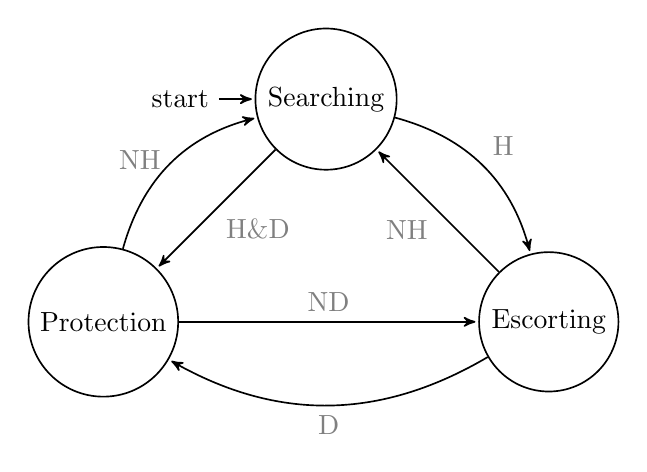
\begin{tikzpicture}[->, >=stealth', shorten >=1pt, auto, node distance=4cm, semithick]
				\node[initial,state] (RW)                    {Searching};
		  		\node[state]         (E) [below right of=RW] {Escorting};
		  		\node[state]         (P) [below left of=RW] {Protection};
		  		
		  		\path	(RW)	 edge[bend left] node{\color{gray} H} (E)
		  				(RW)	 edge node{\color{gray} H\&D} (P)
		  				(E) edge node {\color{gray} NH}	(RW)
		  				(E) edge[bend left] node {\color{gray} D}	(P)
		  				(P) edge node {\color{gray} ND}	(E)
		  				(P) edge[bend left] node[yshift=-0.2cm] {\color{gray} NH}	(RW);

			\end{tikzpicture}
			
%			\resizebox{\textwidth}{!}{%
		  				
		\end{minipage}
		\hfill
		\begin{minipage}[c]{.49\textwidth}
		\resizebox{\textwidth}{!}{%
			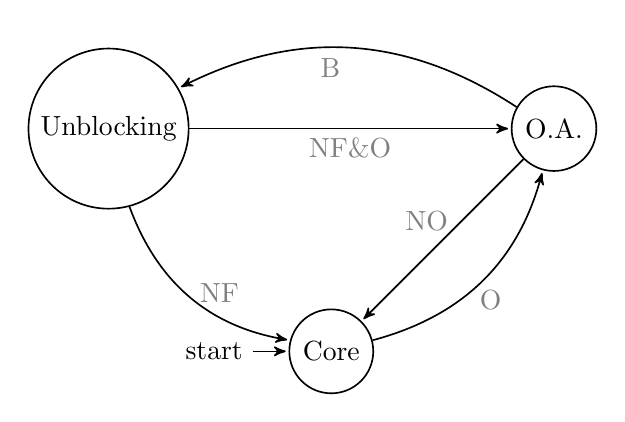
\begin{tikzpicture}[->, >=stealth', shorten >=1pt, auto, node distance=4cm, semithick]
				\node[initial,state] (C)                    {Core};
		  		\node[state]         (O) [above right of=C] {O.A.};
		  		\node[state]         (U) [above left of=C] {Unblocking};
		  		
		  		\path	(C)	edge[bend right] node[below,xshift=0.1cm]{\color{gray} O} (O)
		  				(O) edge node[above,xshift=-0.2cm] {\color{gray} NO}	(C)
		  				(O) edge[bend right] node {\color{gray} B}	(U)
		  				(U) edge node[below] {\color{gray} NF\&O}	(O)
		  				(U) edge[bend right] node[yshift=-0.2cm] {\color{gray} NF}	(C);

			\end{tikzpicture}}
		\end{minipage}
		
		\caption{State machine of the final behaviour}{This figure is the visual representation of the state machine of the final behaviour. Figure \ref{fig:state_machine} (left) is what could be called the \enquote{core} of the behaviour, while Figure \ref{fig:state_machine} (right) would be considered as additions to enhance the behaviour. The core part of the state machine is present on Figure \ref{fig:state_machine} (right) since it is one of its constituents. It is composed of 3 states: \emph{Searching} when the robots do not detect any human nor obstacle, \emph{Escorting} when a human is detected, and \emph{Protection} when a human is detected and there is a danger nearby. If an obstacle is detected by a robot, the controller changes its state to the \emph{Obstacle Avoidance (O.A.)} state. If the robot gets blocked, another state takes over to unblock it: \emph{Unblocking}. When no more obstacle is in front of the robot, it can go back to its obstacle avoidance if any obstacle remains close. If none, it switches back to its core actions. The labels next to each transition must be read as follows: H(uman), D(anger), O(bstacle), F(ront obstacle), B(locked. The robot detects that it is blocked. See page \pageref{sec:unblocking} for details.). N stands for the negation, so NH means \enquote{no human found}.}
		\label{fig:state_machine}
	\end{figure}
	
	\begin{figure}[!htp]\centering
		\begin{minipage}[c]{.49\textwidth}
	%			\begin{tikzpicture}[->, >=stealth', shorten >=1pt, auto, node distance=4cm, semithick]
	%				\node[initial,state] (NORMAL)                    {Normal};
	%		  		\node[state]         (OBS) [below left of=NORMAL] {Obstacle};
	%		  		\node[state]         (HU) [below of=NORMAL] {Human};
	%		  		\node[state]         (DEF) [below right of=NORMAL] {Default};
	%		  		\node[state]         (BLOCK) [above of=NORMAL]       {Blocked};
	%		  		
	%		  		\path	(BLOCK)		edge		node					{\color{gray} 1}	(NORMAL)
	%		  				(NORMAL)		edge		node[yshift=0.2cm]	{\color{gray} 2}	(OBS)
	%		  				(NORMAL)		edge		node					{\color{gray} 3}	(HU)
	%		  				(NORMAL)		edge		node	[yshift=-0.2cm]	{\color{gray} 4}	(DEF)
	%		  				(OBS)		edge		[bend left]	node		{\color{gray} 5}	(BLOCK)
	%		  				(OBS)		edge		[bend right]	node		{}				(NORMAL)
	%		  				(HU)			edge		[bend right]	node		{}				(NORMAL)
	%		  				(DEF)		edge		[bend right]	node		{}				(NORMAL);
	%			\end{tikzpicture}
	%			
			\resizebox{\textwidth}{!}{%
			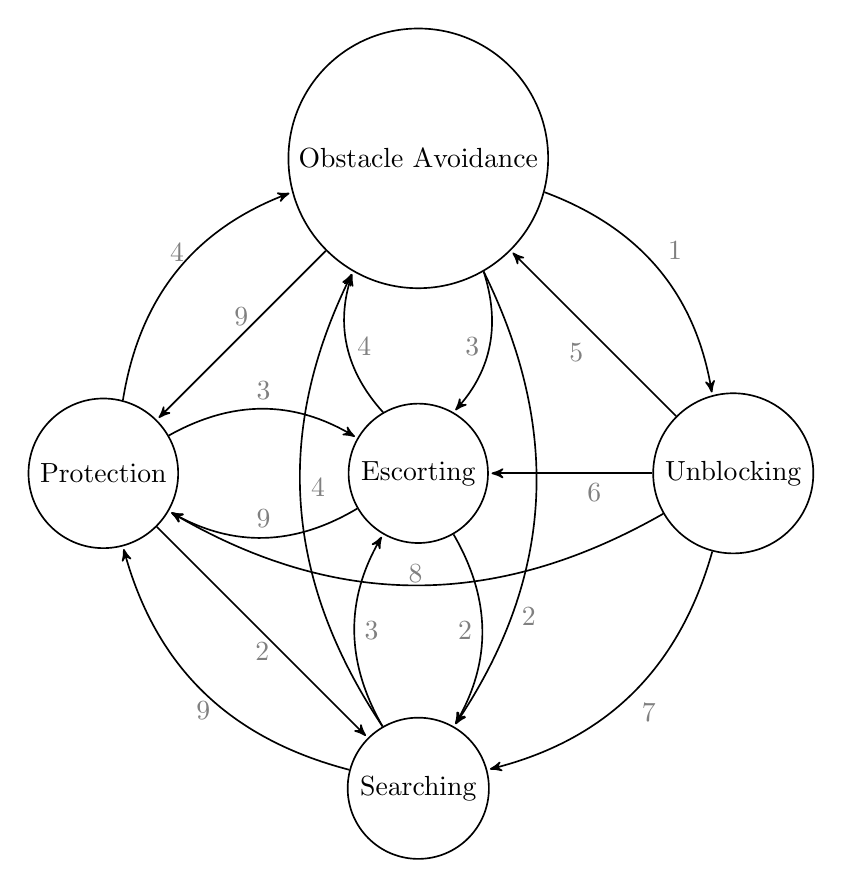
\begin{tikzpicture}[->, >=stealth', shorten >=1pt, auto, node distance=4cm, semithick]
		  		\node[state]         (OBS)					{Obstacle Avoidance};
		  		\node[state]         (HU) [below of=OBS]		{Escorting};
		  		\node[state]         (DEF) [below of=HU]		{Searching};
		  		\node[state]         (BLOCK) [right of=HU]	{Unblocking};
		  		\node[state]         (DANGER) [left of=HU]	{Protection};
		  		
		  		\path	(OBS)		edge	[bend left]	node		{\color{gray} 1}	(BLOCK)
		  				(OBS)		edge	[bend left]	node[yshift=-1.2cm, xshift=-0.3cm]		{\color{gray} 2}				(DEF)
		  				(OBS)		edge	[bend left]	node	[left]	{\color{gray} 3}				(HU)
		  				(HU)			edge	[bend left]	node[right]		{\color{gray} 4}				(OBS)
		  				(HU)			edge	[bend left]	node	[left]	{\color{gray} 2}				(DEF)
		  				(DEF)		edge	[bend left]	node[right]		{\color{gray} 3}				(HU)
		  				(DEF)		edge	[bend left]	node	[right, yshift=0.2cm]	{\color{gray} 4}				(OBS)
		  				(BLOCK)		edge				node		{\color{gray} 5}				(OBS)
		  				(BLOCK)		edge				node	[xshift=0.3cm]	{\color{gray} 6}				(HU)
		  				(BLOCK)		edge	[bend left]			node		{\color{gray} 7}				(DEF)
		  				(BLOCK)		edge	[bend left, above]	node[yshift=-0.1cm]		{\color{gray} 8}				(DANGER)
		  				(HU)		edge	[bend left, above]	node		{\color{gray} 9}				(DANGER)
		  				(DANGER)	 edge[bend left, above] node{\color{gray} 3} (HU)
		  				(DANGER)	 edge[bend left, above] node{\color{gray} 4} (OBS)
		  				(OBS)	 edge[above] node{\color{gray} 9} (DANGER)
		  				(DANGER)	 edge[below] node{\color{gray} 2} (DEF)
		  				(DEF)	 edge[bend left, below] node{\color{gray} 9} (DANGER);
		  				
			\end{tikzpicture}
			}
		\end{minipage}
		\hfill
		\begin{minipage}[c]{.49\textwidth}
			\small\sffamily
			
			\begin{enumerate}
				\item Amount of direction change (left/right) while having an obstacle around reaches a threshold.
				\item No human \& no obstacle.
				\item No obstacle \& human \& no danger.
				\item Obstacle.
				\item No front obstacle \& obstacle elsewhere.
				\item No front obstacle \& human \& no danger.
				\item No front obstacle \& no human \& no obstacle.
				\item No front obstacle \& human \& danger.
				\item No obstacle \& human \& danger.
	
				\end{enumerate}
	
	%			\begin{enumerate}
	%				\item No more obstacle in front.
	%				\item Obstacle found around the robot.
	%				\item Human found around the robot.
	%				\item Neither of the previous criteria met.
	%				\item Amount of direction change (left/right) while having an obstacle around reaches a threshold.
	%			\end{enumerate}
		\end{minipage}
		
		\caption{Complete state machine of the final behaviour}{This figure is the visual representation of the complete state machine of the final behaviour. On Figure \ref{fig:state_machine_complete} (left), the states and their connections are drawn. On Figure \ref{fig:state_machine_complete} (right), the information on the conditions needed to take the transitions are listed.}
		\label{fig:state_machine_complete}
	\end{figure}

	Once the actions the robots have to execute have been defined, we have to implement them, code them in the controller that will be run. So the next step was to find a way to translate those actions into code. Our behaviour is a kind of coordinated motion and pattern formation. Thus the common way of implementing it was to make use of the virtual physics design. Using this framework, each robot is a particle subject to virtual forces exerted by the environment (the other robots, the obstacles, and other elements). \citet{khatib1986real} was among the first to use this method. His goal was to implement an obstacle avoidance swarm behaviour where the obstacles create repulsive forces and the goals attractive forces. The overall resulting potential presented local minima at goals and maxima at obstacles. \citet{reif1999social} introduces \enquote{social potential fields} consisting in virtual forces applied on robots by other robots, obstacles, objectives, or other elements. The robot resultant motion is defined by the sum of all the forces applied to it. The individual robots carry out the calculations themselves, so the final control is completely distributed. The laws they used are similar to those found in molecular dynamics (inverse-power laws). For example, a law could favour attraction over long distances and repulsion over short distances. One of these is the Lennard-Jones potential, depicted in Figure \ref{fig:lennard-jones_potential}. Inverse-power laws, while being extremely simple, can form interesting and elaborate patterns with molecules and plasma gases \citep{reif1999social}. \citet{spears2004distributed} proposed a framework they call \enquote{physicomimetics} to grant distributed control over a large swarm of robots with \enquote{artificial physics}.%\textbf{TODO More works on virtual physics?}
	
	The laws of physics force a system to go to a state of minimum energy, i.e., to reach a minimum of the potential function of the system. Since the force exerted on the system is proportional to the derivative of the corresponding potential -- $$\vec{f} = -\vec{\nabla}P\mbox{,}$$ with $\vec{\nabla}$ being the nabla operator for the gradient computation, $P$ the potential and $\vec{f}$ the force -- the minimum of the potential function means the disappearance of the forces. For every robot to be at the desired location, the forces need to disappear. In this thesis, we only consider forces and not the virtual potentials associated to them. The implemented behaviour is expressed in terms of virtual forces.
	
	\begin{figure}[!htp]
	\begin{minipage}[c]{0.6\textwidth}
		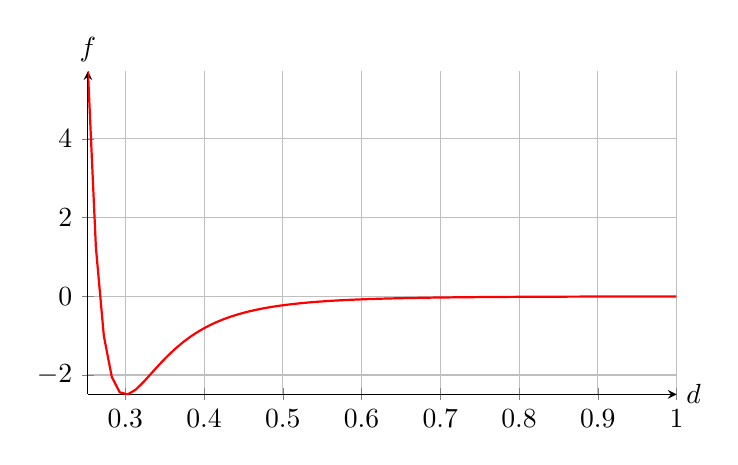
\begin{tikzpicture}
			\begin{axis}[
			    samples=100,
			    domain=0:1, xmax=1,
			    restrict y to domain=-4:10,
			    axis lines=left,
			    y=1cm/2,
			    x=10cm,
			    grid=both,
			    xtick={0,0.1,...,1},
			    ytick={-4,-2,...,10},
			    compat=newest,
			    xlabel=$d$, xlabel style={at={(1,0)}, anchor=west},
			    ylabel=$f$, ylabel style={rotate=-90,at={(0,1)}, anchor=south}
			]
			\addplot [red, thick] {2.5*((0.3/x)^12 - 2*(0.3/x)^6)};
			\end{axis}
		\end{tikzpicture}
	\end{minipage}
	\hfill
	\begin{minipage}[c]{0.4\textwidth}
		$$f(d) = \epsilon \left[ \left(\frac{\sigma}{d}\right)^{12} - 2 \left(\frac{\sigma}{d}\right)^6 \right]$$
		$$\epsilon = 2.5$$
		$$\sigma = 0.3$$
	\end{minipage}
		
		\caption{The Lennard-Jones potential}{This figure shows a graph of one of the most used virtual potentials in virtual physics, the Lennard-Jones potential, where $\epsilon$ is the gain, $\sigma$ is the target distance and $d$ is the current real distance. In this example, the equilibrium is reached at the global minimum at $0.3$.}
		\label{fig:lennard-jones_potential}
	\end{figure}
	
	Using virtual physics offers some advantages over the other methods \citep{brambilla2013swarm}:
	
	\begin{enumerate}
		\item Only one mathematical formula fluently and elegantly converts all the inputs into outputs for the actuators. It removes the need for multiple rules and behaviours.
		$$f:\mathbb{R}^m \rightarrow \mathbb{R}^n:x_1,x_2,...,x_m \rightarrow y_1,y_2,...,y_n = f(x_1,x_2,...,x_m)\mbox{,}$$ where $m$ is the number of inputs, $n$ is the number of outputs and $f$ is the translating function.
		
		\item Multiple behaviours can be combined by simply summing the corresponding resulting vectors.
		$$y_1,y_2,...,y_n = g(x_1,x_2,...,x_m) = \sum_{i=0}^{s}{f_i(x_1,x_2,...,x_m)}\mbox{,}$$ where $s$ is the number of behaviour components.
	\end{enumerate}
One disadvantage is that it might be difficult to find an expression that implements perfectly the behaviour we want.
	
	As written above, the robots need inputs to compute the values to send to the actuators, i.e., the wheels. The two types of inputs are the \emph{colour blobs} and the \emph{proximity sensor values}, respectively provided by the omnidirectional camera and the proximity sensors. Both are explained in section \ref{sec:e-puck}. Three blob colours are used for our solution: red, green and blue, the three basic components of every colour in computer graphics. It was decided to a low number of colours to ease the calibration process and lower the amount of errors when detecting the blobs (wrong colour). To each blob is associated a distance - angle couple. The angle is taken from the front of the robot in radians. With these two values, the robot is able to situate all the blobs and use them as attractive or repulsive points. The proximity values are a list of 8 angle - value couples, where the angle is the position of the sensor on the perimeter of the robot. The whole perimeter of the robot is covered to detect any nearby obstacle. The value is comprised between 0 and 1, inversely proportional to the distance to the obstacle.
	
	The following paragraphs explain in details the various forces that were implemented to obtain the desired behaviour from the given inputs. They are grouped by states of the state machine in which they are used (see fig. \ref{fig:state_machine}). As explained on page \pageref{def:implementation_layers}, each state in the upper layer of the general behaviour (the state machine) contains a sub-behaviour (a particular action) executed by means of virtual physics.
		
			\paragraph{Searching}
			
				When no human nor obstacle is around, the robot enters in the \emph{Searching} mode with its LED off. It tries to stay at a constant distance from a detected colour blob, whatever colour it is. Since robots in \emph{Escorting} or \emph{Protecting} mode light their LEDs in blue, the searching robots always stay around the robots helping the human, whom they will detect at some point. This measure prevents the robots from going away too far from the human. This sub-behaviour is implemented through a sum of simplified Lennard-Jones virtual forces, one for each colour blob detected. The term \enquote{simplified} is used because the force is not the real derivative of the Lennard-Jones potential, but a simplified version with lower exponents on the fractions:% \textbf{TODO Why a simplified version? Put the development.}
				\begin{equation}
					\vec{f}(d) = \frac{-4\epsilon}{d} \left[ \left(\frac{\sigma}{d}\right)^{4} - \left(\frac{\sigma}{d}\right)^2 \right] ~\vec{1_s}
					\label{eq:lennard-jones_force_simplified}
				\end{equation}
				
				The original version is:
				\begin{equation}
					\vec{f}(d) = \frac{-12\epsilon}{d} \left[ \left(\frac{\sigma}{d}\right)^{12} - \left(\frac{\sigma}{d}\right)^6 \right] ~\vec{1_s}
				\end{equation}
				 The simplified version is exposed in Figure \ref{fig:lennard-jones_force_simplified}. If no blob is detected, the robot goes forward with a speed of 5 cm/s. The unit vector $\vec{1_s}$ is heading towards the source of the force (the applier).
				
				\begin{figure}[!htp]\centering
					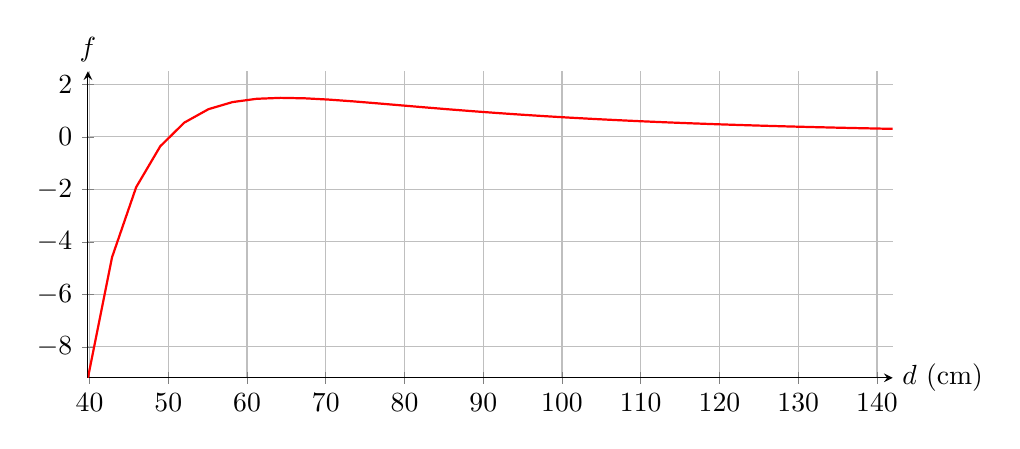
\begin{tikzpicture}
						\begin{axis}[
						    samples=50,
						    domain=0:150, xmax=142, ymax=2.5,
						    restrict y to domain=-10:30,
						    axis lines=left,
						    y=1cm/3,
						    x=1cm/10,
						    grid=both,
						    xtick={0,10,...,150},
						    ytick={-10,-8,...,30},
						    compat=newest,
						    xlabel=$d$ (cm), xlabel style={at={(1,0)}, anchor=west},
						    ylabel=$f$, ylabel style={rotate=-90,at={(0,1)}, anchor=south}
						]
						\addplot [red, thick] {-400/x*((50/x)^4-(50/x)^2)};
						\end{axis}
					\end{tikzpicture}
					
					\caption{The simplified Lennard-Jones virtual force}{This figure exposes a simplified version of the Lennard-Jones force derivated from the corresponding potential. Its expression is given by equation \ref{eq:lennard-jones_force_simplified}. The parameters values are: $\epsilon=100$ and $\sigma=50$, and are conform to those used with robots. One can observe the root at 50 corresponding to the state of minimum energy in the system. Above 50, the force is positive, so the robot is attracted by the source applying the force. Below 50, it is negative, so the robot is repulsed from the source of the force.}
					\label{fig:lennard-jones_force_simplified}
				\end{figure}
			
			\paragraph{Escorting}
			
			If a human is found nearby and no danger is around, the controller enters into the \emph{Escorting} state. The robot then tries to stay at a fixed distance from the human and other robots. If all the robots around the human follow the same pattern formation rules, a circle appears encircling him/her. The complete virtual force for this state is the sum of 3 components: the \emph{human force}, the \emph{robot repulsion force} and the \emph{gravity force}. All three components are fed with the detected colour blobs as inputs to evaluate the distances and angles.
			
			\begin{itemize}
				\item The \emph{human force} uses a stronger version of the Lennard-Jones force to keep the robot at a certain distance from the human (see Figure \ref{fig:lennard-jones_force_stronger}). Its expression is given by equation \ref{eq:lennard-jones_force_stronger}. Only the closest human colour blob is fed to the force computation.
				
					\begin{equation}
						\vec{f}(d) = \left\{ \begin{array}{rcl}
						\frac{-4\epsilon}{d} \left[ \left(\frac{\sigma}{d}\right)^{4} - \left(\frac{\sigma}{d}\right)^2 \right] ~\vec{1_s} & \mbox{for} & d < \sigma \\
						15(d - \sigma ) ~\vec{1_s} & \mbox{for} & d \geq \sigma
						\end{array}\right.
						\label{eq:lennard-jones_force_stronger}
					\end{equation}
				
					\begin{figure}[!htp]\centering
						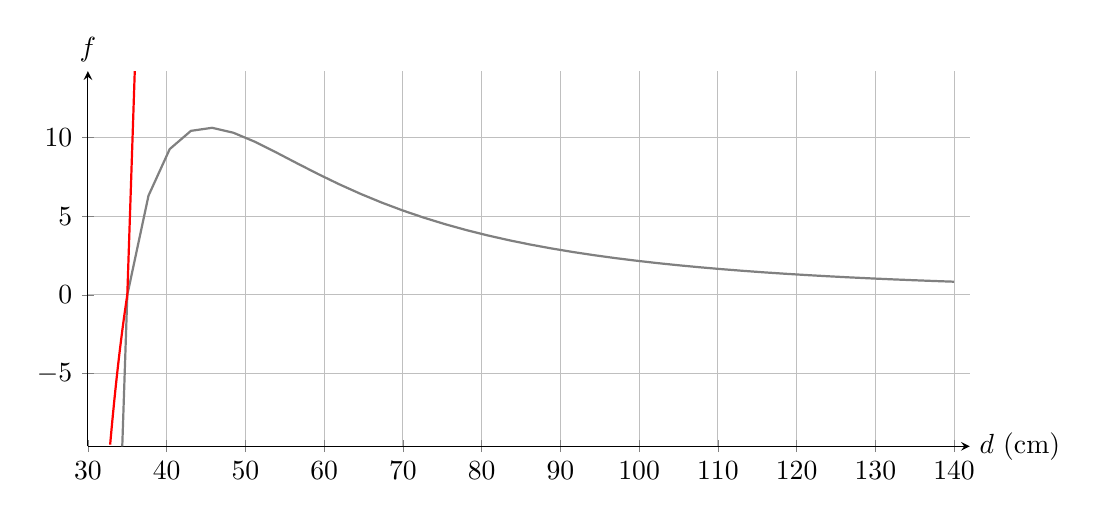
\begin{tikzpicture}
							\begin{axis}[
							    samples=40,
							    domain=30:140, xmax=142, xmin=30, ymax=14.2,
							    restrict y to domain=-10:30,
							    axis lines=left,
							    y=1cm/5,
							    x=1cm/10,
							    grid=both,
							    xtick={30,40,...,150},
							    ytick={-10,-5,...,30},
							    compat=newest,
							    xlabel=$d$ (cm), xlabel style={at={(1,0)}, anchor=west},
							    ylabel=$f$, ylabel style={rotate=-90,at={(0,1)}, anchor=south}
							]
							\addplot [gray, thick, domain=35:140] {-2000/x*((35/x)^4-(35/x)^2)};
							\addplot [gray, thick, domain=30:35] {(x - 35)*15};
							\addplot [red, thick, domain=30:35] {-2000/x*((35/x)^4-(35/x)^2)};
							\addplot [red, thick, domain=35:40] {(x - 35)*15};
							\end{axis}
						\end{tikzpicture}
						
						\caption{The stronger Lennard-Jones virtual force}{This figure exposes a stronger version of the Lennard-Jones force derivated from the corresponding potential. Its expression is given by the equation system \ref{eq:lennard-jones_force_stronger}. The functions are plotted on the whole domain but only the red part is used. It allows to compare the two values for the same distance. The force is stronger in the attraction part, hence the name. The repulsion part is unchanged because of the more interesting asymptotic behaviour at $d=0$, increasing the norm of the force quicker than the linear attraction replacement (in gray). The parameters values are: $\epsilon=500$ and $\sigma=35$, and are conform to those used with robots. One can observe the root at 35 corresponding to the state of minimum energy in the system. Above 35, the force is positive, so the robot is attracted by the source applying the force. Below 35, it is negative, so the robot is repulsed from the source of the force.}
						\label{fig:lennard-jones_force_stronger}
					\end{figure}
				
				\item The \emph{robot repulsion force} maintains a fixed distance between the robots escorting or protecting a human (those with LEDs lit in blue). The simplified Lennard-Jones force is used, given by Equation \ref{eq:lennard-jones_force_simplified} and Figure \ref{fig:lennard-jones_force_simplified}.
				\item The \emph{gravity force} pushes the robots in front of the human like if the floor was \enquote{sloped down} to the front of the human, hence the name. Figure \ref{fig:gravity_force_idea} illustrates the idea of the gravity force and Figure \ref{fig:gravity_force} its norm. This force is expressed in polar coordinates:
				
				\begin{equation}
					\vec{f}(\alpha) = \left\{ \begin{array}{rcl}
						\epsilon ~\vec{1_\theta} & \mbox{for} & \alpha < 0 \\
						-\epsilon ~\vec{1_\theta} & \mbox{for} & \alpha \geq 0
						\end{array}\right.
				\end{equation}
				
				$\vec{1_\theta}$ is the standard axis in polar coordinates ($\vec{1_r},\vec{1_\theta}$) where the origin is the centre of the human. $\epsilon$ is the norm of the force. This force can be deactivated in the configuration file. Sometimes it might not be needed, like in the experiments without human in chapter \ref{chap:experiments}, or when the robots do not need to be pushed in front of the human.
				
				\begin{figure}[!htp]\centering
					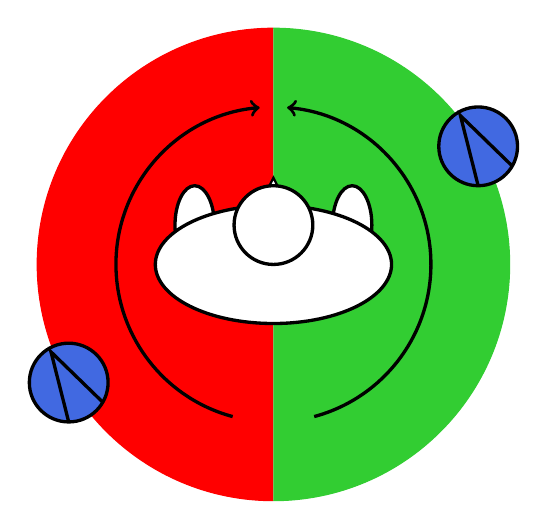
\begin{tikzpicture}						
						\draw[red, fill] (0,3) arc (90:270:3cm);	
						\draw[LimeGreen, fill] (0,3) arc (90:-90:3cm);
						
						\draw[<-, very thick, rotate around={5:(0,0)}] (0,2) arc (90:250:2cm);
						\draw[<-, very thick, rotate around={-5:(0,0)}] (0,2) arc (90:-70:2cm);
						
						\epuckblue[30]{2.6}{1.5}
						\epuckblue[30]{-2.6}{-1.5}
						
						\human{0}{0}
					\end{tikzpicture}
					
					\caption{The gravity virtual force concept}{This figure illustrates the idea of the gravity virtual force. This force that can be disabled in the configuration of the experiment if there is no need to push the robot in front of the human. The closest human colour blob to the human is taken as reference (the closest shoe). Then depending on colour of the blob (shoe), two different things can happen: the blob is red and the robot turns clockwise around it, or the blob is green and the it turns anti-clockwise. The goal is to go in front of the human like if the floor was \enquote{sloped down} to the front of the human, hence the name. Two robots are both on the opposite side of the human. The left one sees the red shoe as the closest one and turns clockwise heading for the front. The right robot does the opposite with the same intention.}
					\label{fig:gravity_force_idea}
				\end{figure}
				
				\begin{figure}[!htp]\centering
					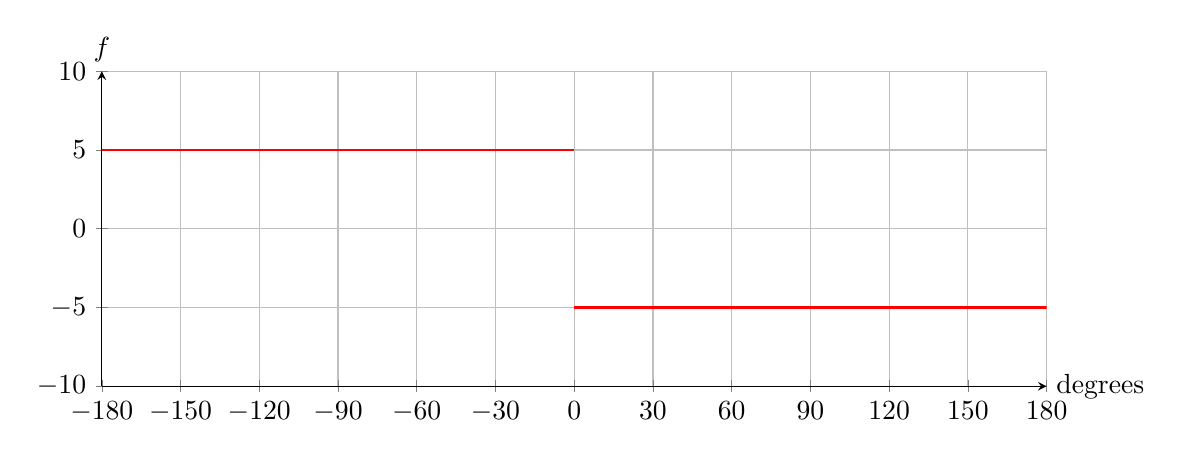
\begin{tikzpicture}
						\begin{axis}[
						    samples=40,
						    domain=-180:180, xmax=180, ymax=10,ymin=-10,
						    restrict y to domain=-10:10,
						    axis lines=left,
						    y=1cm/5,
						    x=1cm/30,
						    grid=both,
						    xtick={-180,-150,...,180},
						    ytick={-10,-5,...,10},
						    compat=newest,
						    xlabel=degrees, xlabel style={at={(1,0)}, anchor=west},
						    ylabel=$f$, ylabel style={rotate=-90,at={(0,1)}, anchor=south}
						]
						\addplot [red, thick, domain=-180:0] {5};
						\addplot [red, thick, domain=0:180] {-5};
						\end{axis}
					\end{tikzpicture}
					
					\caption{The gravity virtual force}{This depicts the adopted value for the gravity virtual force with respect to the angle from the front of the human. Any angle outside this domain can fall back in the $[-180;180]$ interval by normalising it. An angle of 0° means that the robot is in front of the human. The angle increases by turning anti-clockwise.}
					\label{fig:gravity_force}
				\end{figure}
			\end{itemize}
			
		
			\paragraph{Protection}
			
			The \emph{Protection} is reached when the robot detects a human and a danger. It makes its blue LEDs blink and stays at the border of the encountered danger area while maintaining the escorting formation. Hence this sub-behaviour is based on the one from the \emph{Escorting} state. The only difference is in the \emph{human virtual force}. Since everything stays the same as in \emph{Escorting}, except the fact that the robot must not cross the danger border, we just modify the target distance from the human. In presence of a danger, $\sigma$ (the target distance) will be decreased incrementally until no danger is detected any more. As a result, the robot gets closer to the human like seen on Figure \ref{fig:swarm_preventing} at page \pageref{fig:swarm_preventing}. We speak about \emph{dynamic target distance}. Figure \ref{fig:dynamic_target_distance} illustrates the concept. %On the figure, the same robot is represented at two different time steps. On the right, the robot is inside the dangerous area after the human took a step towards it. The robot enters \emph{protection mode} and starts blinking. Its human target distance begins to decrease incrementally at each time step by a user-defined amount. As a consequence, it comes closer to the human. When it crosses the border of the danger zone, it goes back to \emph{Escorting} mode (the danger is not detected any more) and raises its target distance again. At some point, it will re-enter in the area and the whole process will start over. To avoid human confusion regarding the presence of danger, there is a delay before the robot stops blinking. That way, when the robot oscillates around the border, it keeps blinking to report the close danger.
			
			\begin{figure}[!htp]\centering
				\begin{tikzpicture}
					
					\draw[white, fill] (0,-1) rectangle (4,3);
					\draw[red, fill] (4,-1) rectangle (8,3);
					
					\draw[->, very thick] (1,2.5) -- (3.5,2.5);
					\draw[<-, very thick] (4.5,2.5) -- (7,2.5);
					
					\draw (2,-0.5) node[scale=1]{Target $\nearrow$};
					\draw (6,-0.5) node[scale=1]{Target $\searrow$};
					
					\draw[dashed, LightGray] (4,3) -- (0,3) -- (0,-1) -- (4,-1);
				
								\draw[dashed, very thick] (4,-1.5) -- (4,3.5);
					
					\draw (4.5,3.5) node[scale=1, anchor=west]{\textsc{Danger}};
					\draw (3.5,3.5) node[scale=1, anchor=east]{\textsc{Safe}};
					
					
					\human[-90]{-1}{1}
					\epuckblue[-90]{2}{1}
					\epuckblue[90]{6}{1}
					
					\draw (4,1) node[scale=2, anchor=east]{$\leadsto$};
					\draw (4,1) node[scale=2, anchor=east, rotate=180]{$\leadsto$};
					
					\foreach \i in {15,45,...,345} {
				        \draw [very thick, white, rotate around={\i:(6,1)}] (6.6,1) -- (6.9,1);
				    }
								
				\end{tikzpicture}
				
				\caption{The dynamic target distance}{The concept of dynamic target distance is explained in this drawing. On the figure, the same robot is represented at two different time steps. On the right, the robot is inside the red dangerous area after the human took a step towards it. The robot enters \emph{protection mode} and starts blinking. Its human target distance begins to decrease incrementally at each time step by a user-defined amount. As a consequence, it comes closer to the human. When it crosses the border of the danger zone, it goes back to \emph{Escorting} mode (the danger is not detected any more) and raises its target distance again. At some point, it will re-enter in the area and the whole process will start over. To avoid human confusion regarding the presence of danger, there is a delay before the robot stops blinking. That way, when the robot oscillates around the border, it keeps blinking to report the close danger.}
				\label{fig:dynamic_target_distance}
			\end{figure}
			
			\paragraph{Obstacle Avoidance}
			
			The \emph{Obstacle Avoidance} is activated when the robot encounters an object. Since the robot cannot go back, only the front sensors are used. Figure \ref{fig:obstacle_avoidance} shows the four sensors that are taken into account and explains how the state is activated.
			
			\begin{figure}[!htp]\centering
				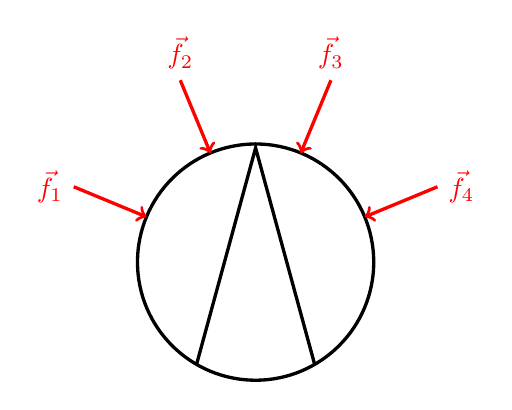
\begin{tikzpicture}
					
					\draw [very thick, fill=white] (0,0) circle [radius=1.5];
					\draw [very thick] (-0.75,-3*0.433) -- (0,1.45) -- (0.75,-3*0.433);
					
					\draw [<-,very thick,red,rotate around={157.5:(0,0)}] (1.5,0) -- (2.5,0) node [left] {$\vec{f_1}$};
					\draw [<-,very thick,red,rotate around={112.5:(0,0)}] (1.5,0) -- (2.5,0) node [above] {$\vec{f_2}$};
					\draw [<-,very thick,red,rotate around={67.5:(0,0)}] (1.5,0) -- (2.5,0) node [above] {$\vec{f_3}$};
					\draw [<-,very thick,red,rotate around={22.5:(0,0)}] (1.5,0) -- (2.5,0) node [right] {$\vec{f_4}$};
				
				\end{tikzpicture}
				
				\caption{The obstacle avoidance concept}{This figure shows the four sensors that are taken into account to detect a nearby object. Each sensor is seen as a force pushing the robot whose intensity is inversely proportional to the distance to the sensed object. If the norm of the strongest force is over a threshold, the robot goes into \emph{Obstacle Avoidance} and uses the resultant as direction vector.}
				\label{fig:obstacle_avoidance}
				\end{figure}
			
			\paragraph{Unblocking}
			\label{sec:unblocking}
			If the robot stays in \emph{Obstacle Avoidance} and changes its direction for some time, it enters into \emph{Unblocking} mode. Figure \ref{fig:unblocking} shows a situation likely to provoke it. The robot enters a narrow path between obstacles. Let us say that it is closer to the left object and goes towards it. Since the forces generated by the proximity sensors on the left are stronger, the resultant is heading to the right, bringing the robot to the other obstacle. The same event occurs on the right side, and the robot returns to the left obstacle. If the robot keeps doing for a certain amount of time, the \emph{Unblocking} mode is activated. At that point, two different things can occur: an obstacle lies ahead of the robot within a certain distance, or nothing is in front of the robot.
			\begin{itemize}
				\item If there is nothing, the robot moves forward for one time step, and returns to the appropriate state: \emph{Obstacle Avoidance} if there is an obstacle around, or a state of the \emph{core} if none.
				\item If there is an obstacle in front, the robot turns on itself until there is none. It is the case in Figure \ref{fig:unblocking}.
			\end{itemize}
			\begin{figure}[!htp]\centering
				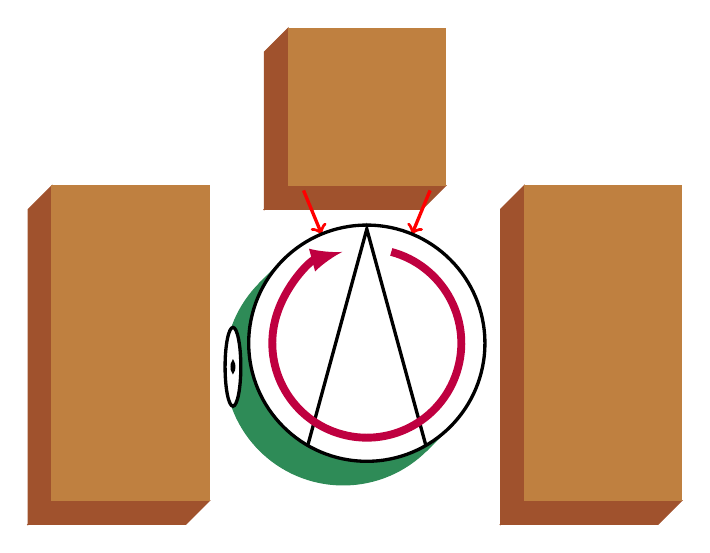
\begin{tikzpicture}					
					
					\draw [Sienna, fill] (-4,2) -- (-4.3,1.7) -- (-4.3,-2.3) -- (-4,-2) -- cycle;
					\draw [Sienna, fill] (-4,-2) -- (-4.3,-2.3) -- (-2.3,-2.3) -- (-2,-2) -- cycle;
					
					\draw [Sienna, fill] (2,2) -- (1.7,1.7) -- (1.7,-2.3) -- (2,-2) -- cycle;
					\draw [Sienna, fill] (2,-2) -- (1.7,-2.3) -- (3.7,-2.3) -- (4,-2) -- cycle;
					
					\draw [Sienna, fill] (-1,4) -- (-1.3,3.7) -- (-1.3,1.7) -- (-1,2) -- cycle;
					\draw [Sienna, fill] (-1,2) -- (-1.3,1.7) -- (0.7,1.7) -- (1,2) -- cycle;
					
					\draw [<-,very thick,red,rotate around={112.5:(0,0)}] (1.5,0) -- (2.1,0);
					\draw [<-,very thick,red,rotate around={67.5:(0,0)}] (1.5,0) -- (2.1,0);
					
						
					\draw [SeaGreen, fill] (-0.3,-0.3) circle [radius=1.5];
					\draw [SeaGreen, fill] (-1.0606601715,1.0606601715) -- (-1.0606601715-0.3,1.0606601715-0.3) -- (-0.3+1.0606601715,-0.3-1.0606601715) -- (1.0606601715,-1.0606601715) -- cycle;
					\draw [very thick, fill=white] (0,0) circle [radius=1.5];
					\draw [very thick] (-0.75,-3*0.433) -- (0,1.45) -- (0.75,-3*0.433);
					\draw[very thick, fill=white] (-1.7,-0.3) ellipse (0.1cm and 0.5cm);
					\draw[very thick, fill] (-1.7,-0.3) ellipse (0.01cm and 0.05cm);
					
					\draw[brown, fill] (-2,-2) rectangle (-4,2);
					\draw[brown, fill] (2,-2) rectangle (4,2);
					\draw[brown, fill] (-1,2) rectangle (1,4);
					
					\draw[->,line width=0.1cm, purple, >=latex, rotate around={-15:(0,0)}] (0,1.2) arc (90:-240:1.2);
					
				\end{tikzpicture}
				
				\caption{The unblocking concept}{On this figure, the robot is trapped between two obstacles, one on the left and the other on the side. Let us say that it is closer to the left object and goes towards it. Since the forces generated by the proximity sensors on the left are stronger, the resultant is heading to the right, bringing the robot to the other obstacle. The same event occurs on the right side, and the robot returns to the left obstacle. If the robot keeps doing for a certain amount of time, the \emph{Unblocking} mode is activated. At that point, two different things can occur: an obstacle lies ahead of the robot within a certain distance, or nothing is in front of the robot. If there is nothing, the robot moves forward for one time step, and returns to the appropriate state: \emph{Obstacle Avoidance} if there is an obstacle around, or a state of the \emph{core} if none. If there is an obstacle in front, the robot turns on itself until there is none. Here, it will turn until heading south of the image, and then get out.}
				\label{fig:unblocking}
			\end{figure}
All the parameters presented until now can be tuned by the human to ensure the best performance. Here is a list of the important parameters available inside the configuration file:
		
	\begin{description}
		\item[Human Force Gain:] The factor $\epsilon$ multiplying the force in expression \ref{eq:lennard-jones_force_stronger}. Increasing it strengthens the force the human exerts on the robots.
		\item[Human Force Distance:] The target distance to the human for all the robot escorting him/her.
		\item[Human Force Distance Variation Delta:] The value added or subtracted to the target distance to run the dynamic target distance mechanism.
		\item[Agent Force Gain:] The factor $\epsilon$ multiplying the force in expression \ref{eq:lennard-jones_force_simplified}. Increasing it strengthens the force robots exert on each other.
		\item[Agent Force Distance:] The target distance all the robots must keep between each other.
		\item[Gravity Force:] A boolean activating the \emph{gravity force} that pushes robots in front of the human.
		\item[Gravity Force Gain:] The norm of the force that pushes the robots in front of the human.
		\item[Direction Vector Window Size:] The direction vector sent to the wheels is computed by averaging a number of direction vectors: the one returned from the forces exerted on the robot at this time step, and a number of previous vectors sent to the wheels. The parameter gives the amount of vectors used for the average. Increasing it makes the motion smoother.
	\end{description}
Once the direction vector has been computed by the robot, it still has to translate it into wheel speeds. As mentioned in section \ref{sec:e-puck}, it has two diametrically opposed wheels. Figure \ref{fig:direction_vector_wheel_speeds_translation} exposes in pseudo code the algorithm behind the conversion.
	
		\begin{algorithm}
			\textcolor{gray}{\tcc{Get the direction values:}}
			\emph{angle} $:=$ angle of the direction vector with respect to the front of the robot\;
			\emph{speed} $:=$ norm of the direction vector\;
			
			\BlankLine
	
			\textcolor{gray}{\tcc{Check if speed is not too high for the robot:}}
			\If{speed > 10}{
				\emph{speed} = 10\;
			}
			
			\BlankLine
			
			\textcolor{gray}{\tcc{Multiply angle by 3 to accelerate the robot rotations:}}
			\emph{angle} = $3~\cdot$ \emph{angle}\;
	
			\BlankLine
			
			\textcolor{gray}{\tcc{Check if angle is still correct:}}
			\If{angle > $\pi$}{
				\emph{angle} = $\pi$\;
			}
			\If{angle < $-\pi$}{
				\emph{angle} = $-\pi$\;
			}
			
			\BlankLine
			
			\textcolor{gray}{\tcc{Assign wheels speed:}}
			\eIf{0 < angle < $\pi$}{
				\emph{leftWheelSpeed} = \emph{speed} $\cdot\cos($\emph{angle}$)$\;
				\emph{rightWheelSpeed} = \emph{speed}\;
			}{
				\emph{leftWheelSpeed} = \emph{speed}\;
				\emph{rightWheelSpeed} = \emph{speed} $\cdot\cos($\emph{angle}$)$\;
			}
			
					\caption{The direction vector to wheel speeds translation}{This pseudo code explains how the computed direction vector is translated into the robot wheel speeds. The speed limit for the e-pucks is about 10 cm/s. Thus, the first action after getting the direction vector is to limit its norm. The angle of the vector is then multiplied by a factor to accelerate the rotation of the robots. The idea behind the rotation algorithm is to reduce the speed of the wheel corresponding to the direction of the rotation. E.g.: if the robot needs to turn left, the left wheel speed decreases by a factor proportional to the angle. The function that best fits is the cosinus of the angle, decreasing from 1 at 0° to -1 when the angle is 180°, making the robot progressively increase the curvature of the path from straight line to rotation on itself.}
		\label{fig:direction_vector_wheel_speeds_translation}
		\end{algorithm}
		

	

%////////////////////////////////////////////////////////////
\chapter{Experiments}
%////////////////////////////////////////////////////////////
\label{chap:experiments}
\begin{comment}
[\textcolor{red}{Explain very clearly both types of tests (no human/human).}]
\end{comment}

In this chapter, we introduce the different experiments we conducted with the real robots. These experiments were conducted with the E-puck robotic platform \citep{mondada2009puck}. We can classify the experiments into two sets: one assessing the system quantitatively, and one assessing the system qualitatively (i.e., the demonstration). We first describe the quantitative assessments, and their results in the section \ref{sec:characterisation_system}. Then we switch to the other kind of experiments in the section \ref{sec:demonstration}.

	\section{Characterisation of the System}
	\label{sec:characterisation_system}
	\begin{comment}
		[The measurements and the tests on the final behaviour.]
	\end{comment}
	
	In this section, we assess the performance of our solution without any human controlling the swarm. The solution is evaluated quantitatively and qualitatively with 5 criteria. In this section, we introduce these criteria.
	
		\subsection{The Robot Speed}
			
			The robots have a speed limit. Their wheel speed cannot be higher than 10 cm/s (0.36 km/h). This limit has been fixed as one of the best practices by the laboratory staff to ensure that the robots do not get damaged in an experiment. The average walk speed of a human is 5 km/h \citep{wiki:002}. The experiments that will follow can thus be seen as proof of concept. Faster robots would be required for real application. Furthermore, the robots should be able to move around in multiple kinds of environments. The E-puck \citep{mondada2009puck} is only suited for flat surfaces.
	
		\subsection{The Shoe Detection Range}
		
			In this section, we determine the range of detection of the shoes by the robots. We determine the maximum distance at which the robots see the shoes. Figure \ref{fig:shoe_detection_range} illustrates the experiment we conducted to determine this distance. The maximal distance goes from 59 cm in front and behind the shoes, to 65 cm on the right and 70 cm on the left. This distance is acceptable given the size of the robots. It gives enough room to the user. There is no risk of stepping on a robot. The probable cause of the lower distance for the green shoe is the lower intensity of the green LEDs inside the shoe. We use a lower luminosity to increase the recognition rate of the green shoe by the robots. A brighter green shoe leads to a more difficult calibration and worse blob detection rate on the robots.
						
			\begin{figure}[!htp]\centering
			\begin{tikzpicture}
			
				\draw[Yellow, fill] (-1,2) rectangle (-1.3,4.5);
				\foreach \i in {2.1,2.3,...,4.5} {
			        \draw [very thin,Black] (-1,\i) -- (-1.2,\i);
			    }
			    \epuckblue[180]{0}{4.5}
			    \draw (-1.3,4.5) node[scale=2, anchor=east]{60 cm$\leadsto$};
			    
			    \draw[Yellow, fill] (1,-2) rectangle (1.3,-4.5);
				\foreach \i in {-2.1,-2.3,...,-4.5} {
			        \draw [very thin,Black] (1,\i) -- (1.2,\i);
			    }
			    \epuckblue[-90]{-5}{0}
			    \draw (-5,-1.3) node[scale=2, anchor=east, rotate=90]{70 cm$\leadsto$};
			    
			    \draw[Yellow, fill] (-2.35,-1) rectangle (-5,-1.3);
				\foreach \i in {-2.45,-2.65,...,-5} {
			        \draw [very thin,Black] (\i,-1) -- (\i,-1.2);
			    }
			    \epuckblue{0}{-4.5}
			    \draw (4.75,1.3) node[scale=2, anchor=west, rotate=90]{~~~~~65 cm};
			    \draw (4.75,1.3) node[scale=2, anchor=east, rotate=270]{$\leadsto$};
			    
			    \draw[Yellow, fill] (2.35,1) rectangle (4.75,1.3);
				\foreach \i in {2.45,2.65,...,4.75} {
			        \draw [very thin,Black] (\i,1) -- (\i,1.2);
			    }
			    \epuckblue[90]{4.75}{0}
			    \draw (1.3,-4.5) node[scale=2, anchor=west]{~~~~~60 cm};
			    \draw (1.3,-4.5) node[scale=2, anchor=east, rotate=180]{$\leadsto$};
			    
				\draw[red, fill] (-0.5,-2) rectangle (-2.35,2);
				\draw[LimeGreen, fill] (0.5,-2) rectangle (2.35,2);
				
				\draw[BurlyWood, fill] (-0.73,-1.77) rectangle (-2.12,1.77);
				\draw[BurlyWood, fill] (0.73,-1.77) rectangle (2.12,1.77);	
				
			\end{tikzpicture}
			\caption{The shoe detection range}{This figure depicts the experiment we conducted to evaluate the maximum distance from the shoes at which the robots detect the shoes. A robot was placed on the left, right, front and behind the shoes. We manually incrementally moved the robot closer to the shoes until the robot detected them. We measured the corresponding distance to the shoes. The red shoe is the left shoe, and the green one is the right one.}
			\label{fig:shoe_detection_range}
			\end{figure}
			
		\subsection{Circle Properties}
			In this section, we evaluate the properties of the circle formed by the swarm of robots. We first expose the three metrics we used to perform the evaluations. Then we detail the conditions of the experiments. Finally, we analyse the observations made with the experiments.
			
			\subsubsection{Metrics}
			\label{sec:circle_properties_metrics}
			\begin{comment}
				[Metrics I will use. Their description. How I will compute them.]
			\end{comment}
			
			In order to evaluate the performance of our solution, we needed to create metrics to put numbers on the behaviour observed (how we compute the performance of our solution). We defined three metrics which we think correspond the most to what we want to capture from the observations: \emph{Correct Distance}, \emph{Robot Density} and \emph{Time}.
			
			\begin{enumerate}
				\item \emph{Correct Distance}. This metric measures to what extent the robotic swarm respects the target distance to the human.
				\item \emph{Robot Density}. It measures how regularly spaced the robots are around the human. The more regularly spaced they are, the best it is. It checks if the human is protected from all directions.
				\item \emph{Time}. It measures how long it takes for the swarm to reach a configuration such that the \emph{Correct Distance} and \emph{Robot Density} metrics go under a given threshold.
			\end{enumerate}
			
				\paragraph{Correct Distance}
					\begin{comment}
						[Do the robots respect the correct wanted distance?]
					\end{comment}
					
					This metric measures to what extent the robotic swarm respects the target distance to the human. To measure the error related to the distance human-robot, we consider the distance from every robot to the rectangle formed by the two shoes (see Figure \ref{fig:distance_metric}). Once we have these distances, we use the next formula to compute an error for every time step:
					\begin{equation}
						\mbox{error}_t = \frac{1}{N} \sum_{i=1}^N \frac{|d_{ti} - \overline{d}|}{\overline{d}},
						\label{eq:distance_metric}
					\end{equation}
					
					 where $t$ is the number of the time step, $N$ is the number of robots, $d_{ti}$ is the distance human-robot for robot $i$ at time step $t$, and $\overline{d}$ is the target distance. Since the detected colour blob on the shoe might not always be the nearest point to the robot in the rectangle, this error measure is not perfect. Indeed, the robot adjusts its distance based on the closest human colour blob, not on the closest point of the shoe (perimeter of the rectangle). Although this error measure is not perfect, it is still reasonable enough for our purpose. To measure the error between the real distance and the target distance, the robots use the colour blobs on the shoes. One blob may cover a big part of one shoe. This is caused by the diffusion of the light in the plexiglass material we used for the shoes. So its center might not be the closest point to the robot on the shoe itself. On the other side, the measure of the error we make with the arena tracking system takes as reference the closest point to the robot on the shoe itself. There is thus a difference between the way the robot computes its error and adjusts its position with respect to the human, and the way we compute the error afterwards. It would be difficult to use the same methodology to compute the error, as the arena tracking system cannot see the colour blobs. We would have to compute the error on each robot separately, and then gather all the data to get the final value. In that case, however, the measure would not come from an outside device. It would come from the robots themselves. This would be less interesting because if there is an error in the distance measure in the robot, the error measure would be good but in reality the robot would be misplaced.
					 %It is difficult to measure the distance between each robot and each human colour blob. The arena tracking system \citep{stranieri2013iridia} cannot see the colour blobs. The only way would be to compute it directly on each robot separately, then merge all the data afterwards. In that case, however, the measure does not come from an outside device. It comes from the robots themselves. This is less interesting because if there is an error in the distance measure in the robot, the error measure would be good but in reality the robot would be misplaced.
					
					\begin{figure}[!htp]\centering
						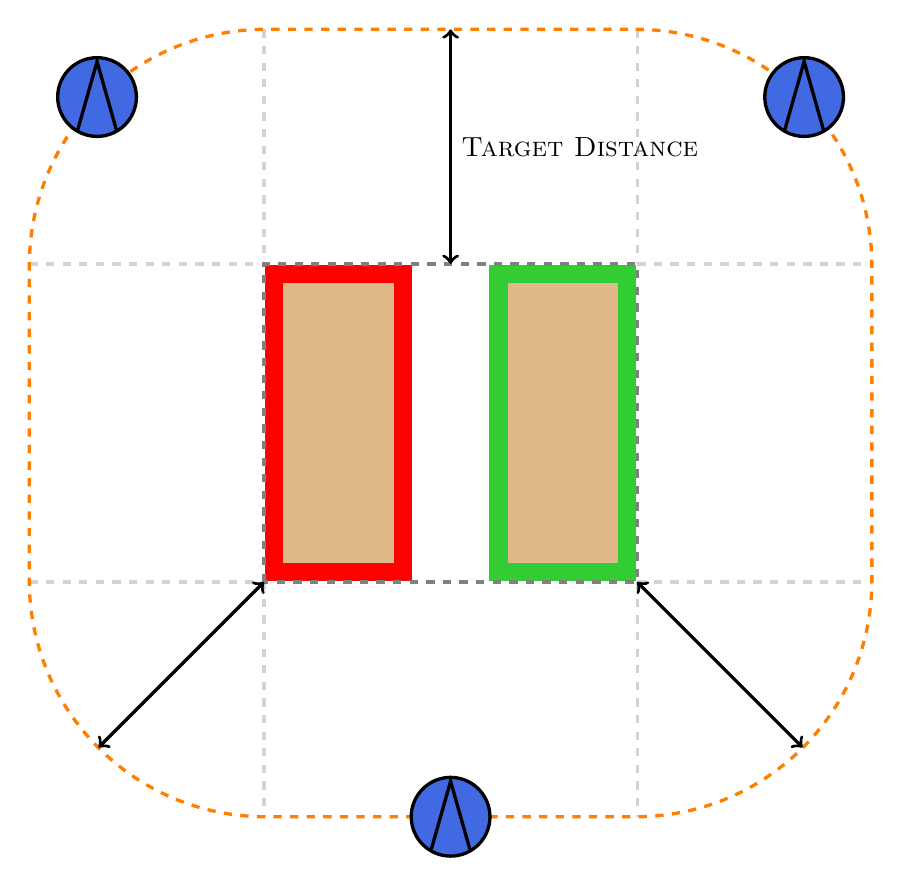
\begin{tikzpicture}
						
						%	\foreach \i in {\xMin,...,\xMax} {
						%        \draw [very thin,gray] (\i,\yMin) -- (\i,\yMax)  node [below] at (\i,\yMin) {$\i$};
						%    }
						%    \foreach \i in {\yMin,...,\yMax} {
						%        \draw [very thin,gray] (\xMin,\i) -- (\xMax,\i) node [left] at (\xMin,\i) {$\i$};
						%    }
						
							\draw[red, fill] (-0.5,-2) rectangle (-2.35,2);
							\draw[LimeGreen, fill] (0.5,-2) rectangle (2.35,2);
							
							\draw[BurlyWood, fill] (-0.73,-1.77) rectangle (-2.12,1.77);
							\draw[BurlyWood, fill] (0.73,-1.77) rectangle (2.12,1.77);
							
						%	\draw[dashed, very thick] (-2.35,5) -- (2.35,5);
						%	\draw[dashed, very thick] (-2.35,-5) -- (2.35,-5);
						%	\draw[dashed, very thick] (-5.35,2) -- (-5.35,-2);
						%	\draw[dashed, very thick] (5.35,2) -- (5.35,-2);
						%	\draw[dashed, very thick] (-5.35,2) arc (180:90:3);
						%	\draw[dashed, very thick] (5.35,2) arc (0:90:3);
						%	\draw[dashed, very thick] (-5.35,-2) arc (180:270:3);
						%	\draw[dashed, very thick] (5.35,-2) arc (0:-90:3);
						
							\draw[dashed, very thick, LightGray] (-2.37, 5) -- (-2.37, 2.02);
							\draw[dashed, very thick, LightGray] (-2.37, -2.02) -- (-2.37, -5);
							\draw[dashed, very thick, LightGray] (2.37, 5) -- (2.37, 2.02);
							\draw[dashed, very thick, LightGray] (2.37, -2.02) -- (2.37, -5);
							\draw[dashed, very thick, LightGray] (-5.35, 2.02) -- (-2.37, 2.02);
							\draw[dashed, very thick, LightGray] (2.37, 2.02) -- (5.35, 2.02);
							\draw[dashed, very thick, LightGray] (-5.35, -2.02) -- (-2.37, -2.02);
							\draw[dashed, very thick, LightGray] (2.37, -2.02) -- (5.35, -2.02);
							\draw[dashed, very thick, Gray] (-2.37, -2.02) rectangle (2.37, 2.02);
							
							\draw [dashed, very thick, orange] (2.35,5) to [out=0,in=90] (5.35,2) to [out=270,in=90] (5.35,-2) to [out=270, in=0] (2.35,-5) to [out=180, in=0] (-2.35,-5) to [out=180, in=270] (-5.35,-2) to [out=90, in=270] (-5.35,2) to [out=90, in=180] (-2.35,5) -- cycle;
						
							%\draw[dashed, LightGray] (-2.37,-2.02) rectangle (2.37,2.02);
							
							\draw[<->, very thick] (0,2.02) -- (0,5) node [right] at (0,3.5) {\textsc{Target Distance}};
							\draw[<->, very thick] (-2.37,-2.02) -- (-4.47,-4.12);
							\draw[<->, very thick] (2.37,-2.02) -- (4.47,-4.12);
							
							\epuckblue{0}{-5}
							\epuckblue{-4.49}{4.14}
							\epuckblue{4.49}{4.14}
						\end{tikzpicture}
						
						\caption{The distance metric}{This figure represents the algorithm used to compute the distance metric. The red and green shoes in the middle form a rectangle. The position of all robots is obtained thanks to the arena tracking system (see Appendix \ref{app:arena_tracking_system}). The distance of all robots to the rectangle is computed. We compare every distance to the target human distance (we take absolute value of the difference). Then we divide by the human target distance to normalise. We normalise since an error of 10 cm for a target distance of 30 cm is not the same as an error of 10 cm for a target distance of 100 cm. The average of all those divisions is the error of the current time step. The example depicted on the figure would return an error of 0. See expression \ref{eq:distance_metric}. One can see that the geometric shape formed by the points that are at the target distance from the human is not a perfect circle. This is because the robots position themselves with respect to the shoes, not the center of the human. We try to provide a measure that corresponds to the way robots compute their own distance.}
						\label{fig:distance_metric}
					\end{figure}
				
				\paragraph{Robot Density}
					\begin{comment}
						[Do the robots surround the human correctly?]
					\end{comment}
					
					It measures how regularly spaced the robots are around the human. The more regularly space they are, the more the human is protected from all directions. The error on the angular density of robots is computed as follows. The positions of all the robots are captured, and the angle between each consecutive pair of robots is calculated (see Figure \ref{fig:density_metric}). This list of angles is fed to the next formula to return the error for the current timestep:
					\begin{equation}
						\mbox{error}_t = \frac{1}{N} \sum_{i=1}^N \frac{|\alpha_{ti} - \overline{\alpha}|}{\overline{\alpha}},
						\label{eq:density_metric}
					\end{equation}
					
					where $t$ is the number of the time step, $N$ is the number of robots, $\alpha_{ti}$ is the angle separating the pair of consecutive robots $i$ at time step $t$, and $\overline{\alpha}$ is the target angle.
					
					\begin{figure}[!htp]\centering
						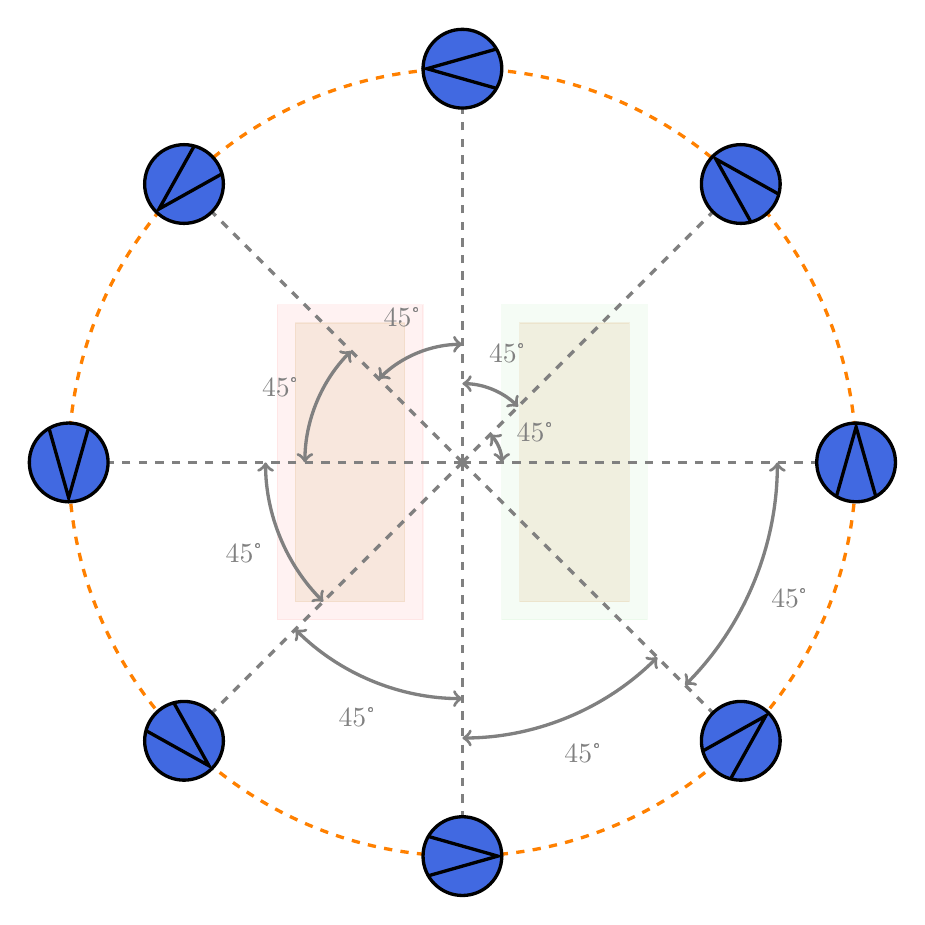
\begin{tikzpicture}
						
						%	\foreach \i in {\xMin,...,\xMax} {
						%        \draw [very thin,gray] (\i,\yMin) -- (\i,\yMax)  node [below] at (\i,\yMin) {$\i$};
						%    }
						%    \foreach \i in {\yMin,...,\yMax} {
						%        \draw [very thin,gray] (\xMin,\i) -- (\xMax,\i) node [left] at (\xMin,\i) {$\i$};
						%    }
						
							\draw[red, fill, opacity=0.05] (-0.5,-2) rectangle (-2.35,2);
							\draw[LimeGreen, fill, opacity=0.05] (0.5,-2) rectangle (2.35,2);
							
							\draw[BurlyWood, fill, opacity=0.2] (-0.73,-1.77) rectangle (-2.12,1.77);
							\draw[BurlyWood, fill, opacity=0.2] (0.73,-1.77) rectangle (2.12,1.77);
						
							\draw[very thick, dashed, orange] (0,0) circle [radius=5cm];
							
							\foreach \i in {0,45,...,315} {
								\draw [very thick, dashed, gray, rotate around={\i:(0,0)}] (0,0) -- (5,0);
								
								\draw [very thick, fill=RoyalBlue, rotate around={\i:(0,0)}] (5,0) circle [radius=0.5];
								\draw [very thick, rotate around={\i:(0,0)}] (5-0.25,-0.433) -- (5,0+0.45) -- (5+0.25,-0.433);
								
								%\draw[rotate around={\i:(0,0)}] (\i*5/360,0) arc [0:30:(\i+45)*4/360];
								\draw [<->, very thick, gray, rotate around={\i:(0,0)}] (\i*4/360+0.5,0) arc [radius=(\i+45)*4/360, start angle=0, end angle=45];
								
								\draw [rotate around={\i+22.5:(0,0)}] (\i*4/360+1,0) node {\textcolor{gray}{45°}};
							}
							
							%\human{0}{0}
						
							
						\end{tikzpicture}
						
						\caption{The density metric}{This figure represents the algorithm used to compute the density metric. The position of all robots with the origin centred on the shoes is obtained thanks to the arena tracking system (see Appendix \ref{app:arena_tracking_system}). Then the angle between every consecutive pair of robots is computed. We compare every angle to the target angle (360°/\#robots, here 45°) by subtracting the second to the first. Then we divide by the target angle to normalise. Normalisation is necessary since an error of 10° for a target of 30° is not the same as an error of 10° for a target of 90°. The average of all those divisions is the error of the current time step. The example depicted on the figure would return an error of 0. See expression \ref{eq:density_metric}.}
						\label{fig:density_metric}
					\end{figure}
					
					
				\paragraph{Time}
				\begin{comment}
					[Do they do that in a relatively low amount of time?]
				\end{comment}
				
				It measures how long it takes for the swarm to reach a configuration such that the \emph{Correct Distance} and \emph{Robot Density} metrics go under a given threshold. To get this value, we average the evolutions of the error over time for every type of experiment. We compare this evolution to a defined threshold representing a certain quality of the solution. We obtain an average time for every type of experiment corresponding to the time step where the threshold is crossed.
				
			\subsubsection{Setup}
			
				\begin{comment}
					How I am performing my experiments. Two types. Pictures. Duration. 8 robots. Dimensions of the arena. Where? Matlab scripts?
				\end{comment}
			
				These experiments took place in the IRIDIA laboratory, in the arena room. The arena room is the place were the academic staff can manipulate the robots and run experiments. We used 8 e-pucks for every experiment. They were all equipped with tags to allow the arena tracking system \citep{stranieri2013iridia} to locate them, and transmit the location to the simulator. At the beginning of each experiment, the robots were placed according to the type of experiment undertaken. There are two types of experiment. The first one consists in a random starting position for all the robots. Figure \ref{fig:random_setup} illustrates the first set-up type. The other type consists in a specific starting position: all the robots are placed on the right of the shoes. The arena is a rectangle, bounded with wood boards or walls (on the right of the picture on the two figures there is a wall). Each experiment lasted 3 minutes. At each time step of the 3 minute long experiment, the positions of robots are saved into a file on the tracking system server. When the experiment is finished, the file is transferred to another computer located in the arena room. All the log files are then filtered by a Matlab script we implemented to remove the errors in the positions. Some robots are indeed misplaced or not found for several time steps due to some tracking system errors. Once the files have been cleaned, other Matlab scripts compute the values for the metrics listed in section \ref{sec:circle_properties_metrics}.
			
				\begin{figure}[!htp]
					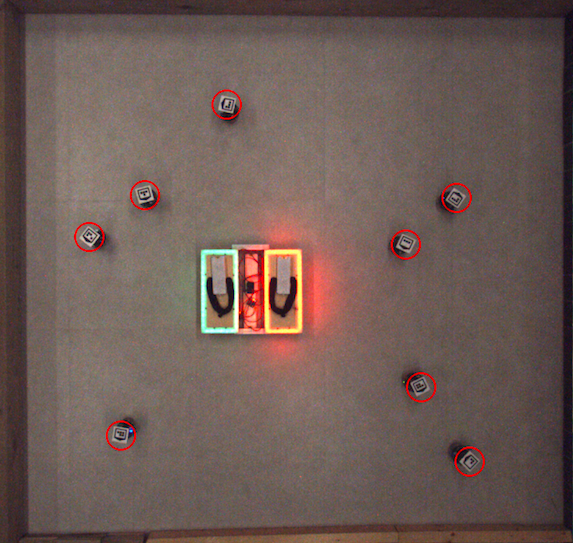
\includegraphics[width=\textwidth]{images/setup_random.png}
					\caption{The random setup}{On this figure, we show an example of a random starting position for all the robots. The initial positions of all the robots are computed by a random plot of 8 points in Matlab, 8 couples (x,y) such that $x \in [-1,1], y \in [-1,1]$. The robots are then manually placed as the points are shown on the Matlab generated plot. The shoes are centred under the camera. The camera is the origin of the environment: $(0,0)$. The origin is not centred on the picture as we cropped the image to keep only the relevant part. The picture was taken from one of the 16 camera of the arena tracking system \citep{stranieri2013iridia}.}
					\label{fig:random_setup}
				\end{figure}
			
				\begin{figure}[!htp]
					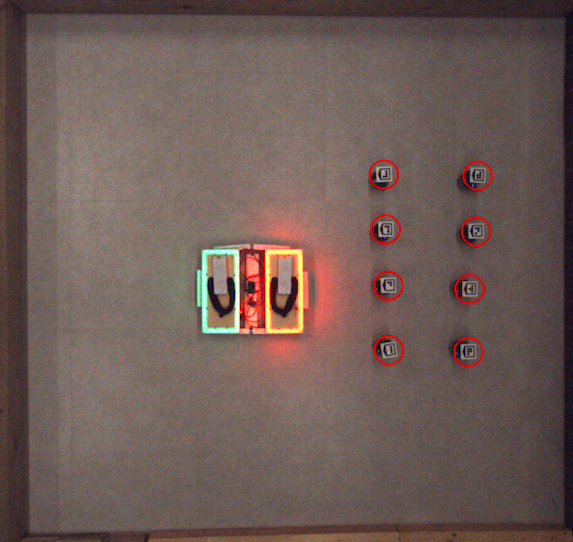
\includegraphics[width=\textwidth]{images/setup_geo.png}
					\caption{The specific setup}{On this figure, we show an example of a specific setup. All the robots are placed on the right of the shoes. This starting configuration is interesting since it could represent the usual configuration where all the robots are stored and waiting for the activity to begin. The shoes are centred under the camera. The camera is the origin of the environment: $(0,0)$. The origin is not centred on the picture as we cropped the image to keep only the relevant part. The picture was taken from one of the 16 camera of the arena tracking system \citep{stranieri2013iridia}.}
					\label{fig:geo_setup}
				\end{figure}
			
			\subsubsection{Analysis}
			
				\begin{comment}
					All the graphs we discussed about. The evolution of the error over time. The analysis of the behaviour on basis of the criteria we defined. Random, side, other geo?, all together.
				\end{comment}
					
					In this section we analyse the information gathered from our experiments. The goal of these experiments was to show that the error measures we defined in section \ref{sec:circle_properties_metrics} are decreasing over time during each experiment and stabilising after some acceptable time. We grouped the results by type of error measure. First we analyse the distance results, then the density results. We end with the time metric. For both types of starting configuration, the results are based on 10 runs of the experiment.
					
					On figures \ref{fig:boxplot_random_distance} and \ref{fig:boxplot_geo_distance}, we show the evolution of the average distance error over time in the context of the random starting point experiment and in the context of the specific starting point configuration. On both figures, we observe a clear decrease of the error over time. On figure \ref{fig:boxplot_random_distance}, the stabilisation is more obvious than for figure \ref{fig:boxplot_geo_distance} where the median continues to decrease slightly at the end of the 3 minutes. Furthermore we can observe that the values of the error are a lot more spread for the specific setup (Figure \ref{fig:boxplot_geo_distance}) than for the random setup (\ref{fig:boxplot_random_distance}). We can explain this observation by the fact that the robots are close to each other at the beginning of the experiment. That, and the nature of the virtual forces exerted on the robots make the robots disperse in almost random directions at the beginning of the experiments. Typically, on figure \ref{fig:geo_setup}, the robots on the right column would disperse to the right because of the column of robots on their left. Although the robots on the right are also attracted by the shoes, the repulsive forces of the robots on the left are stronger. Since for the random start configuration the robots are more likely to be dispersed in the arena, they are less subject to the forces of the other robots. Once the experiment starts, they just move towards the shoes. The behaviours observed during these experiments were not so different, leading to a small distribution for the error value, as seen on figures \ref{fig:boxplot_random_distance} and \ref{fig:boxplot_random_density}. From the distance metric point of view, the random starting position is the best.
			
				\begin{figure}[!htp]
					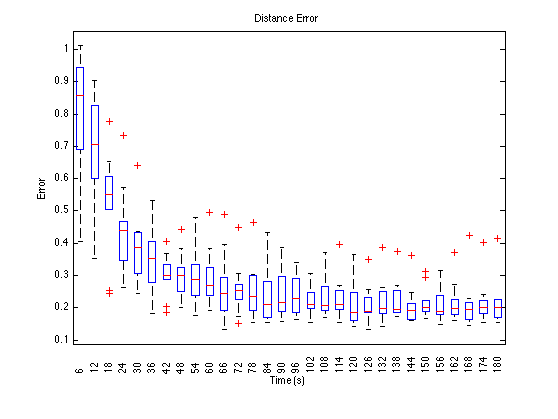
\includegraphics[width=\textwidth]{../MATLAB/boxplot_random_distance.png}
					\caption{The distance error for a random starting configuration}{On this figure, we show the evolution of the average distance error through boxplots. It is an average on 10 experiments with real robots. The initial positions of all the robots are randomly selected. We observe that the behaviour of the swarm tends to lower the error measure. The variance of the values distribution is very low (0.0087 on average). A boxplot is a way of representing the distribution of a group of values. Each box corresponds to one group of values. On each box, one can see the median (the red line) of the distribution. The blue box is the interval between the first quartile and the third quartile: the interquartile range (IQR). The dashed black line is the interval of all the non outlier points. The upper whisker (the upper end of the black line) is the highest datum still within 1.5 IQR of the upper quartile \citep{wiki:003}. The lower whisker is the lowest datum still within 1.5 IQR of the lower quartile. Any point above the upper whisker or below the lower whisker is called outlier.}
					\label{fig:boxplot_random_distance}
				\end{figure}
			
				
				\begin{figure}[!htp]
					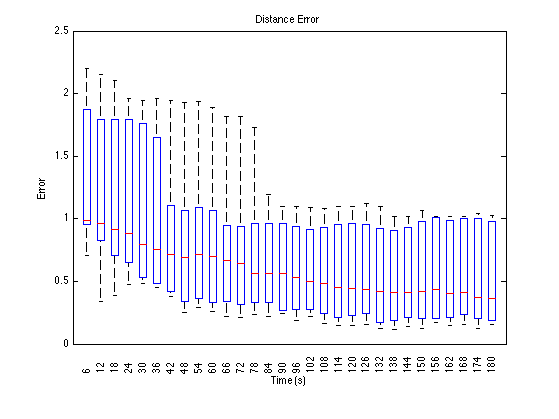
\includegraphics[width=\textwidth]{../MATLAB/boxplot_geo2_distance.png}
					\caption{The distance error for a specific starting configuration}{On this figure, we show the evolution of the average distance error through boxplots. It is an average on 10 experiments with real robots. The robots are placed on a grid on the right of the shoes like shown on Figure \ref{fig:geo_setup}. We observe that the behaviour of the swarm tends to lower the error measure. The variance of the values distribution is very high (0.2034 on average).}
					\label{fig:boxplot_geo_distance}
				\end{figure}
				
				As expected, the density error value is bigger for the specific configuration than for the random starting configuration as the robots are clustered on the right of the shoes (Figure \ref{fig:boxplot_random_density} and \ref{fig:boxplot_geo_density}). The angles separating the robots are further from the target angle (see section \ref{sec:circle_properties_metrics}) than for the random setup. Once again, the values are decreasing over time for the two types of configurations. The values are stabilising after 2 minutes for the random configuration. The specific configuration does not stabilise completely at the end of the 3 minutes. The variance of the values distribution is bigger for the specific configuration (0.0241 for the random configuration, and 0.0560 for the specific one). However the difference is less important than for the distance metric. The error values are higher for the specific configuration. This could be due to the difficulty of the reorganisation undertaken by the robots: half of the robots have to go on the other side of the shoes. In the other configuration, the robots are already more dispersed around the shoes. As for the distance metric, the random configuration is the best alternative.
				
				\begin{figure}[!htp]
					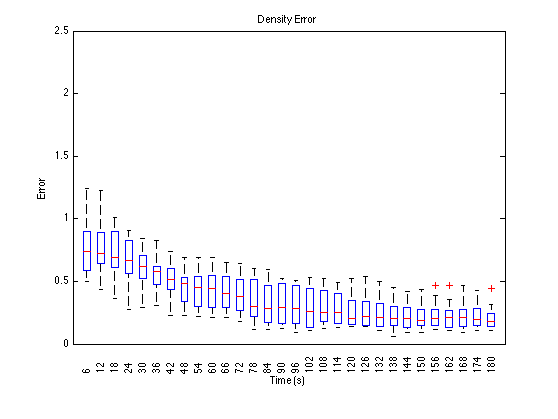
\includegraphics[width=\textwidth]{../MATLAB/boxplot_random_density.png}
					\caption{The density error for a random starting configuration}{On this figure, we show the evolution of the average density error through boxplots. It is an average on 10 experiments with real robots. The initial positions of all the robots are randomly selected. We observe that the behaviour of the swarm tends to lower the error measure. The variance of the values distribution is low (0.0241 on average).}
					\label{fig:boxplot_random_density}
				\end{figure}
			
				
				\begin{figure}[!htp]
					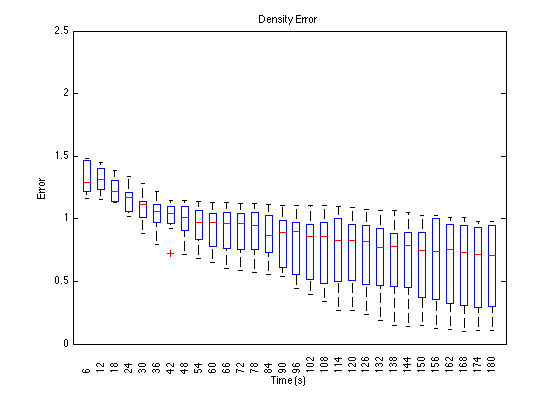
\includegraphics[width=\textwidth]{../MATLAB/boxplot_geo2_density.png}
					\caption{The density error for a specific starting configuration}{On this figure, we show the evolution of the average density error through boxplots. It is an average on 10 experiments with real robots. The robots are placed on a grid on the right of the shoes like shown on Figure \ref{fig:geo_setup}. We observe that the behaviour of the swarm tends to lower the error measure. The variance of the values distribution is high (0.0560 on average).}
					\label{fig:boxplot_geo_density}
				\end{figure}
				
				As the values are not completely stabilising for the specific starting configuration, it was interesting to see what was the evolution of the error for a longer experiment. We thus launched one experiment of 9 minutes with the specific starting configuration. Figure \ref{fig:geolong} (a) and \ref{fig:geolong} (b) show the evolution of the error over time. The two figures show a global decrease of the error value. However, the distance error on Figure \ref{fig:geolong} (a) has a more monotonous evolution than the density one. The latter undergoes an augmentation around 3 minutes. During the first 180 seconds, the two evolutions correspond to what was observed in figures \ref{fig:boxplot_geo_distance} and \ref{fig:boxplot_geo_density}. The two series of values tend to stabilise at 0.8. Figure \ref{fig:geolong} (c) shows the final state of the swarm at the end of the experiment. The robots are forming an acceptable circular shield around the human. One can conclude that 0.8 is a nice value for the error measure. The value 0.8 will thus be used as threshold of quality for the time metric.
				
%				\begin{figure}[!htp]
%					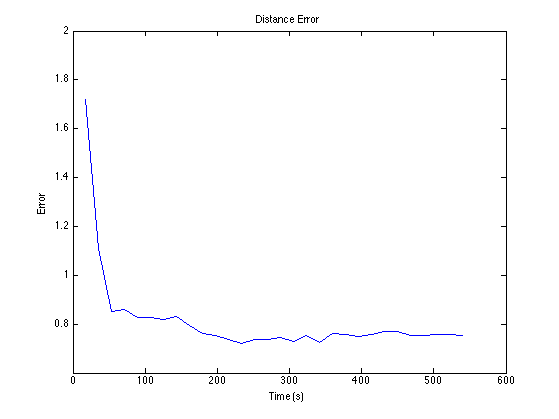
\includegraphics[width=\textwidth]{../MATLAB/boxplot_geolong_distance.png}
%					\caption{The distance error for a specific starting configuration (long experiment)}{On this figure, we show the evolution of the distance error for one run of the experiment. The experiment lasted 9 minutes. One can see a global decrease showing that the behaviour tends to create a circle that presents good characteristics for our application.}
%					\label{fig:geolong_distance}
%				\end{figure}
%			
%				\begin{figure}[!htp]
%					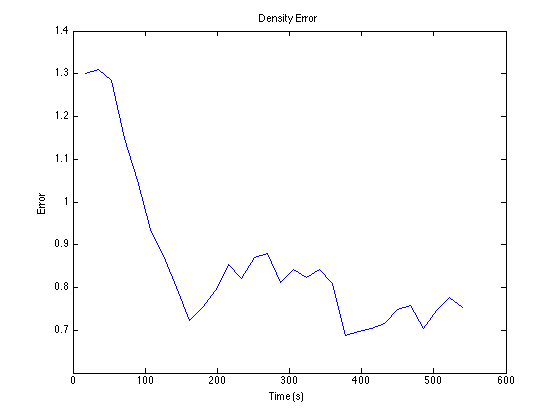
\includegraphics[width=\textwidth]{../MATLAB/boxplot_geolong_density.png}
%					\caption{The density error for a specific starting configuration (long experiment)}{On this figure, we show the evolution of the density error for one run of the experiment. The experiment lasted 9 minutes. One can see a global decrease showing that the behaviour tends to create a circle that presents good characteristics for our application. One can observe an augmentation around 200 seconds. The video from the experiment showed that the robots moved slightly to the right of the shoes, putting more space between the robots on the left. The robots returned to their correct position afterwards, as the graph suggests.}
%					\label{fig:geolong_density}
%				\end{figure}
%				
%				\begin{figure}[!htp]
%					\includegraphics[width=\textwidth]{images/geolong_end.png}
%					\caption{Final state of the 9-minutes experiment}{On this figure, we depict the final state of the 9-minutes experiment using the specific configuration as starting configuration. It corresponds to a value of 0.8 for the two error measures. We defined this value as an acceptable quality.}
%					\label{fig:geolong_final_state}
%				\end{figure}
%				
				\begin{figure}[!htp]
					\begin{minipage}{0.5\textwidth}
						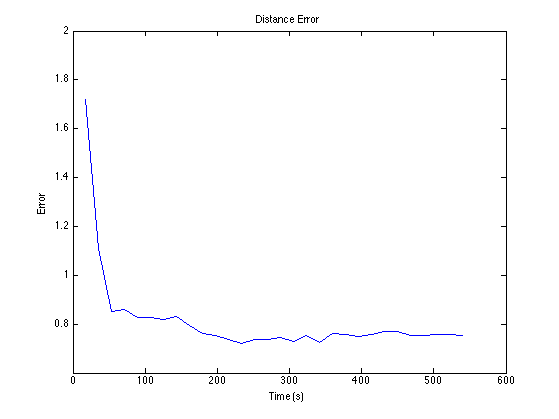
\includegraphics[width=\textwidth]{../MATLAB/boxplot_geolong_distance.png}
						\centering (a)
					\end{minipage}
					\hfill
					\begin{minipage}{0.5\textwidth}
						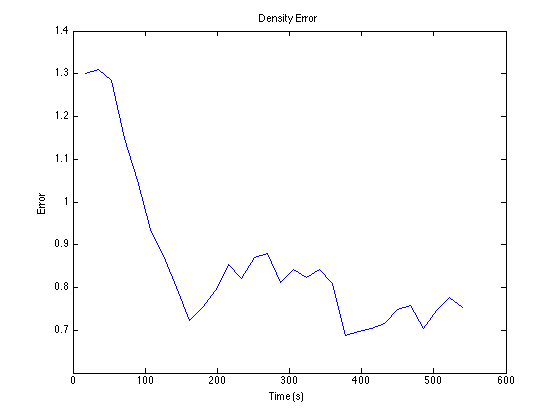
\includegraphics[width=\textwidth]{../MATLAB/boxplot_geolong_density.png}
						\centering (b)
					\end{minipage}
					\center \includegraphics[width=0.5\textwidth]{images/geolong_end.png}
					\center (c)
					
					\caption{The long experiment for the specific starting configuration}{On this figure, we show the evolution of the distance error (a) and the density error (b) for one run of the experiment. The experiment lasted 9 minutes. One can see a global decrease in the two graphs showing that the behaviour tends to create a circle that presents good characteristics for our application. On (b) one can observe an augmentation around 200 seconds. The video from the experiment showed that the robots moved slightly to the right of the shoes, putting more space between the robots on the left. The robots returned to their correct position afterwards, as the graph suggests. (c) depicts the final state of the 9-minutes experiment using the specific configuration as starting configuration. It corresponds to a value of 0.8 for the two error measures. We defined this value as an acceptable quality.}
					\label{fig:geolong}
				\end{figure}
				
				If we use a threshold value of 0.8 for the quality measure, we observe a great difference between the random and specific configuration in the time it takes for the error measure to cross the threshold. Since for the distance and density metrics the best alternative was the random start configuration, it is logical that the alternative taking the less amount of time to cross the threshold of 0.8 is the random alternative. We take the median as reference. If the configuration is random, the swarm takes a few seconds on average to cross the threshold. On the other side, for the specific configuration, the swarm takes approximately 1min30s to do the same for the density metric, and 30 seconds for the distance metric.
				
				As a conclusion, we can say that the random starting configuration is the best in the experiments we performed. It offered a consistent behaviour, as seen on Figure \ref{fig:boxplot_random_distance} and Figure \ref{fig:boxplot_random_density}. The variance is a lot smaller than for the other solution (see Table \ref{tab:variances}). At the end of the experiments, the value for the two types of errors were almost the same. Even if the specific starting configuration is a worse solution than the random starting configuration, the robots still managed to reach a state of acceptable quality in our standards after some time. In future applications, one would thus have to choose between the compactness of the specific configuration, leading to bigger delays, and the speed of the random solution, harder to set up.
				
				
				\begin{table}[!htp]\centering
					\begin{tabular}{|c|c|c|}
					\hline 
					Variances & Distance & Density \\ 
					\hline 
					Random & 0.0087 & 0.0241 \\ 
					\hline 
					Specific & 0.2034 & 0.0560 \\ 
					\hline 
					\end{tabular}
					\caption{The variances}{On this figure we gather all the variances from the experiments we conducted. Each of the 4 values is an average of the variances of one of the 4 experiments.}
					\label{tab:variances}
				\end{table}
			
	\section{Demonstration}
		\label{sec:demonstration}

		In the previous section we performed experiments that did not involve any human. In this section, one human is using the shoes to walk in a virtually dangerous zone and stay protected by the robots. We called this experiment \enquote{the demonstration}. The goal was to check if the robots were able to follow the human and warn him/her about the dangerous areas. It acts as a proof of concept.
		
		\subsection{Setup}
		
			We ran this experiment in the arena room, in the IRIDIA laboratory. We simulated one dangerous area on the floor using the arena tracking system \citep{stranieri2013iridia,reinaaugmented} and ARGoS \citep{pinciroli2012argos,GarFraBruPinBir2015:techreport-004}. Eight E-pucks were used \citep{mondada2009puck}. The experiment was recorded with a digital camera. Only one human took part of the experiment. The human had to walk slowly towards a circular dangerous zone whose diameter was 1 meter. At some point, the robots should notify him/her about the danger. The human would then walk around the dangerous area as depicted on Figure \ref{fig:demo_setup}. The dangerous area was not visible to the human. If the robots would not tell to the human that a danger is nearby, the experiment would fail. The human started the experiment as shown on Figure \ref{fig:demo_setup}, on the left of the dangerous area.
			
			\begin{figure}[!htp]\centering
				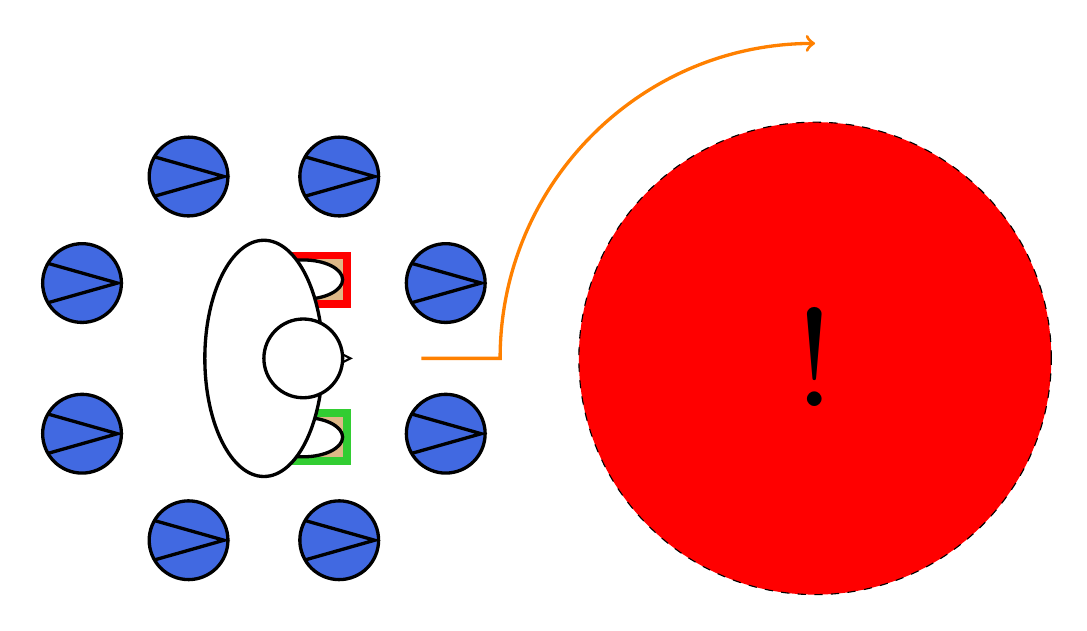
\begin{tikzpicture}
				
					\clip (-7,-3.1) rectangle (6.1, 4.2);
					
					\draw [dashed, fill=red] (3,0) circle [radius=3];
					\draw (3,0) node[scale=5]{!};
					
					\draw[red, fill] (-2.9,0.65) rectangle (-4.1,1.35);
					\draw[LimeGreen, fill] (-2.9,-0.65) rectangle (-4.1,-1.35);
					\draw[BurlyWood, fill] (-3,0.75) rectangle (-4,1.25);
					\draw[BurlyWood, fill] (-3,-0.75) rectangle (-4,-1.25);
					\human[-90]{-4}{0}
					
					\draw [->,very thick, orange] (-2,0) to [out=0,in=180] (-1,0) to [out=90,in=180] (3,4);
					
					\foreach \i in {22.5,67.5,...,347.5} {
						\begin{scope}[rotate around={\i:(-4,0)}]
							\epuckblue[-90-\i]{-1.5}{0}
						\end{scope}
					}
					%\draw [brown] (current bounding box.south west) rectangle (current bounding box.north east);
				\end{tikzpicture}
				
				\caption{The demonstration setup}{On this figure, we show the staring configuration of the demonstration experiment, and the expected path the human has to follow. The human first walk slowly towards the dangerous area (the red disc). He is surrounded by 8 protecting E-pucks that follow him. The human is wearing the two shoes that were built to allow the robots to detect him.}
				\label{fig:demo_setup}
			\end{figure}
			
		\subsection{Analysis}
		
			\begin{comment}
				[What demonstration was done with the device. Add pictures. Describe perfectly.]
			\end{comment}
			
			In this section, we describe the unfolding of the experiment on the basis of pictures taken from the video we recorded. On Figure \ref{fig:demo_pictures}, we present the sequential events that occurred during the experiment. Figure \ref{fig:demo_pictures} (a) shows the starting configuration of the experiment. The human is equipped with the shoes we built. The robots are surrounding him. He is ready to move towards danger. After a few steps, the human has reached the point where the robots see the dangerous area. They notify the danger to him by blinking their LEDs. One can see on Figure \ref{fig:demo_pictures} (b) the two frontal robots blinking (their LEDs are currently off for a short period of time). The human decides to avoid the danger and turns left. While moving around the dangerous area, the robots in contact with it stay blinking. The 3 robots on the right side of the human on Figure \ref{fig:demo_pictures} (c) are touching the dangerous area. Thanks to this feedback sent by the robots, the human knows its relative position to the danger. On this picture, one can also see the mechanism that switches off the LEDs of the shoe working. The left shoe is not touching the ground any more, releasing the switch and opening the circuit powering the LEDs. On Figure \ref{fig:swarm_preventing} we showed how the swarm of robots had to stay on the boundary of the dangerous area, even if the distance between the robots and the human is under the target distance. One can observe on Figure \ref{fig:demo_pictures} (d) that the robots on the right of the human follow the curvature of the dangerous area. On Figure \ref{fig:demo_pictures} (e) the human has the same heading he had at the beginning of the experiment. The danger area is on his right, as signalled by the robots on his right. Soon after, the robots on the right of the human will retrieve their correct distance to the human, and stop blinking. The danger area has been avoided.
			
			\begin{figure}[!htp]
				\begin{minipage}[c]{0.49\textwidth}
					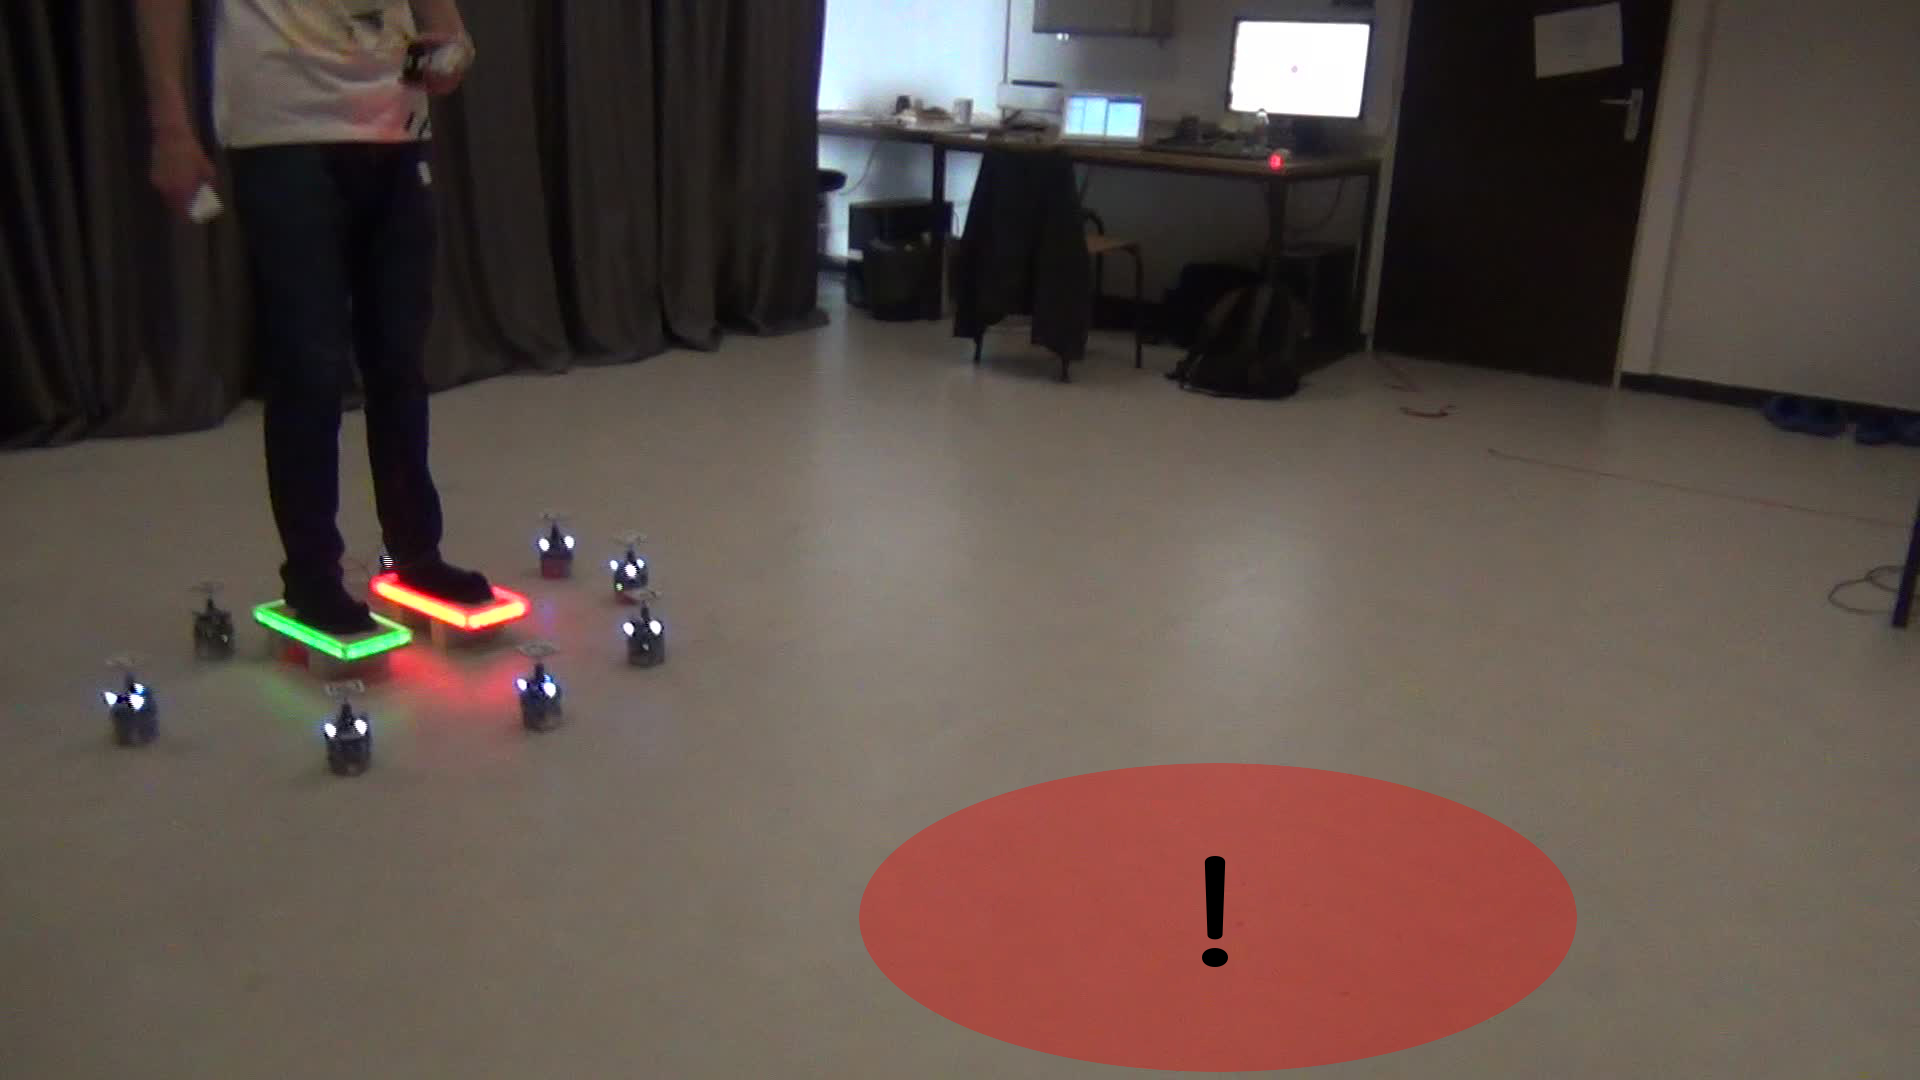
\includegraphics[width=\textwidth]{images/vlcsnap-00001.jpg}
					\centering (a)
				\end{minipage}
				\hfill
				\begin{minipage}[c]{0.49\textwidth}
					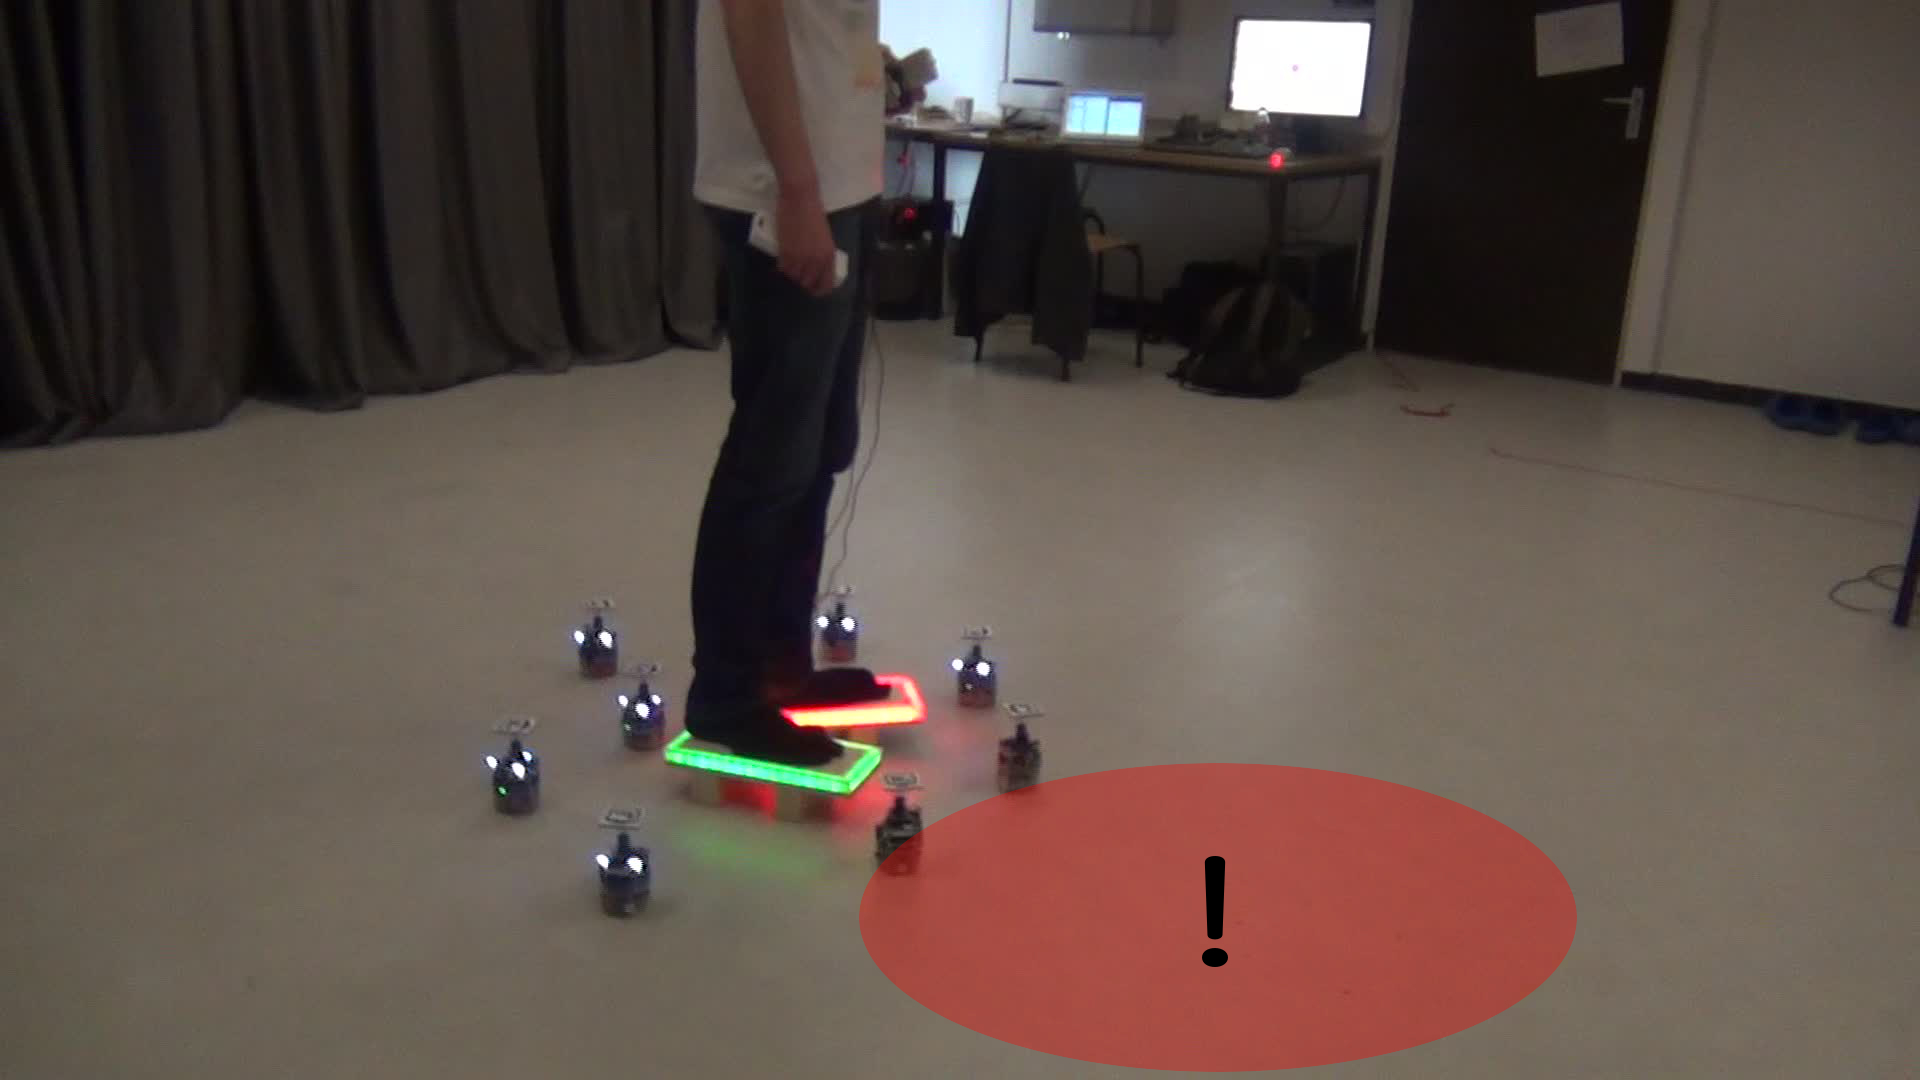
\includegraphics[width=\textwidth]{images/vlcsnap-00002.jpg}
					\centering (b)
				\end{minipage}
				\begin{minipage}[c]{0.49\textwidth}
					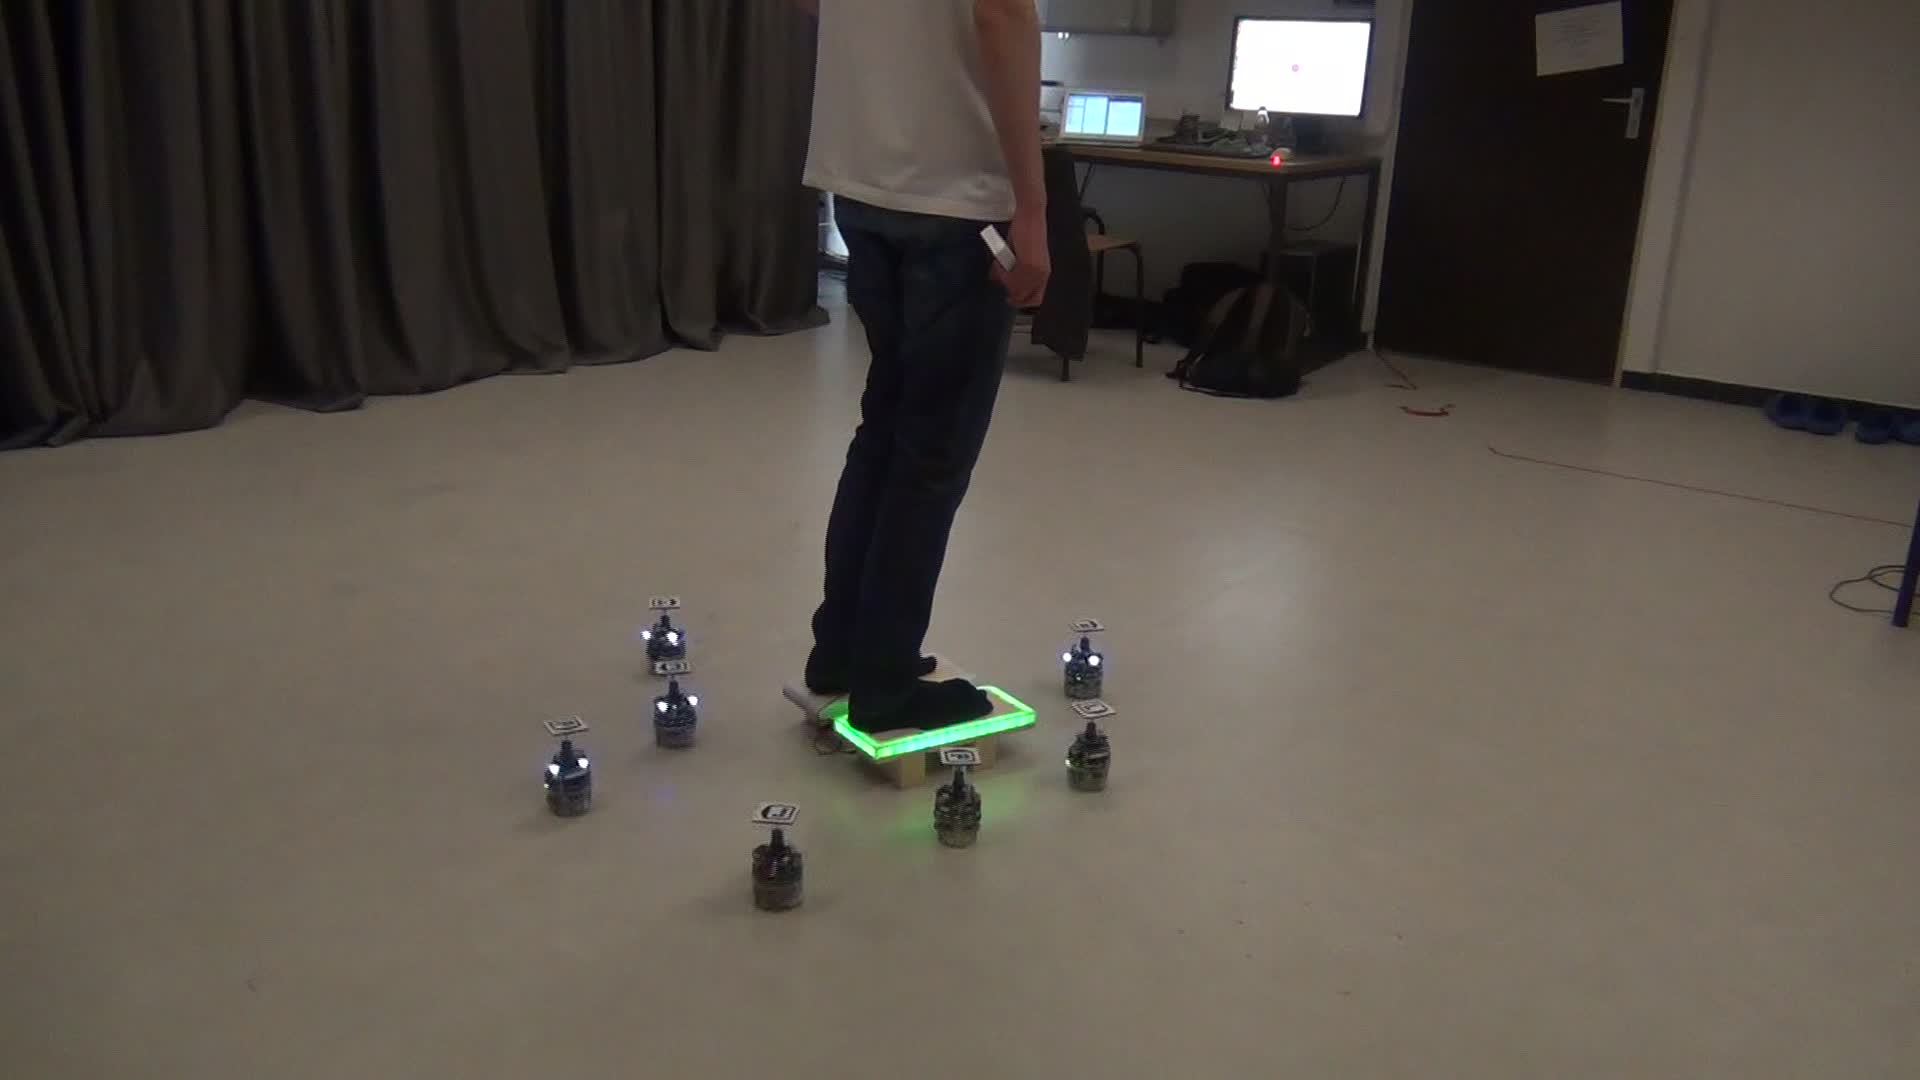
\includegraphics[width=\textwidth]{images/vlcsnap-00003.jpg}
					\centering (c)
				\end{minipage}
				\hfill
				\begin{minipage}[c]{0.49\textwidth}
					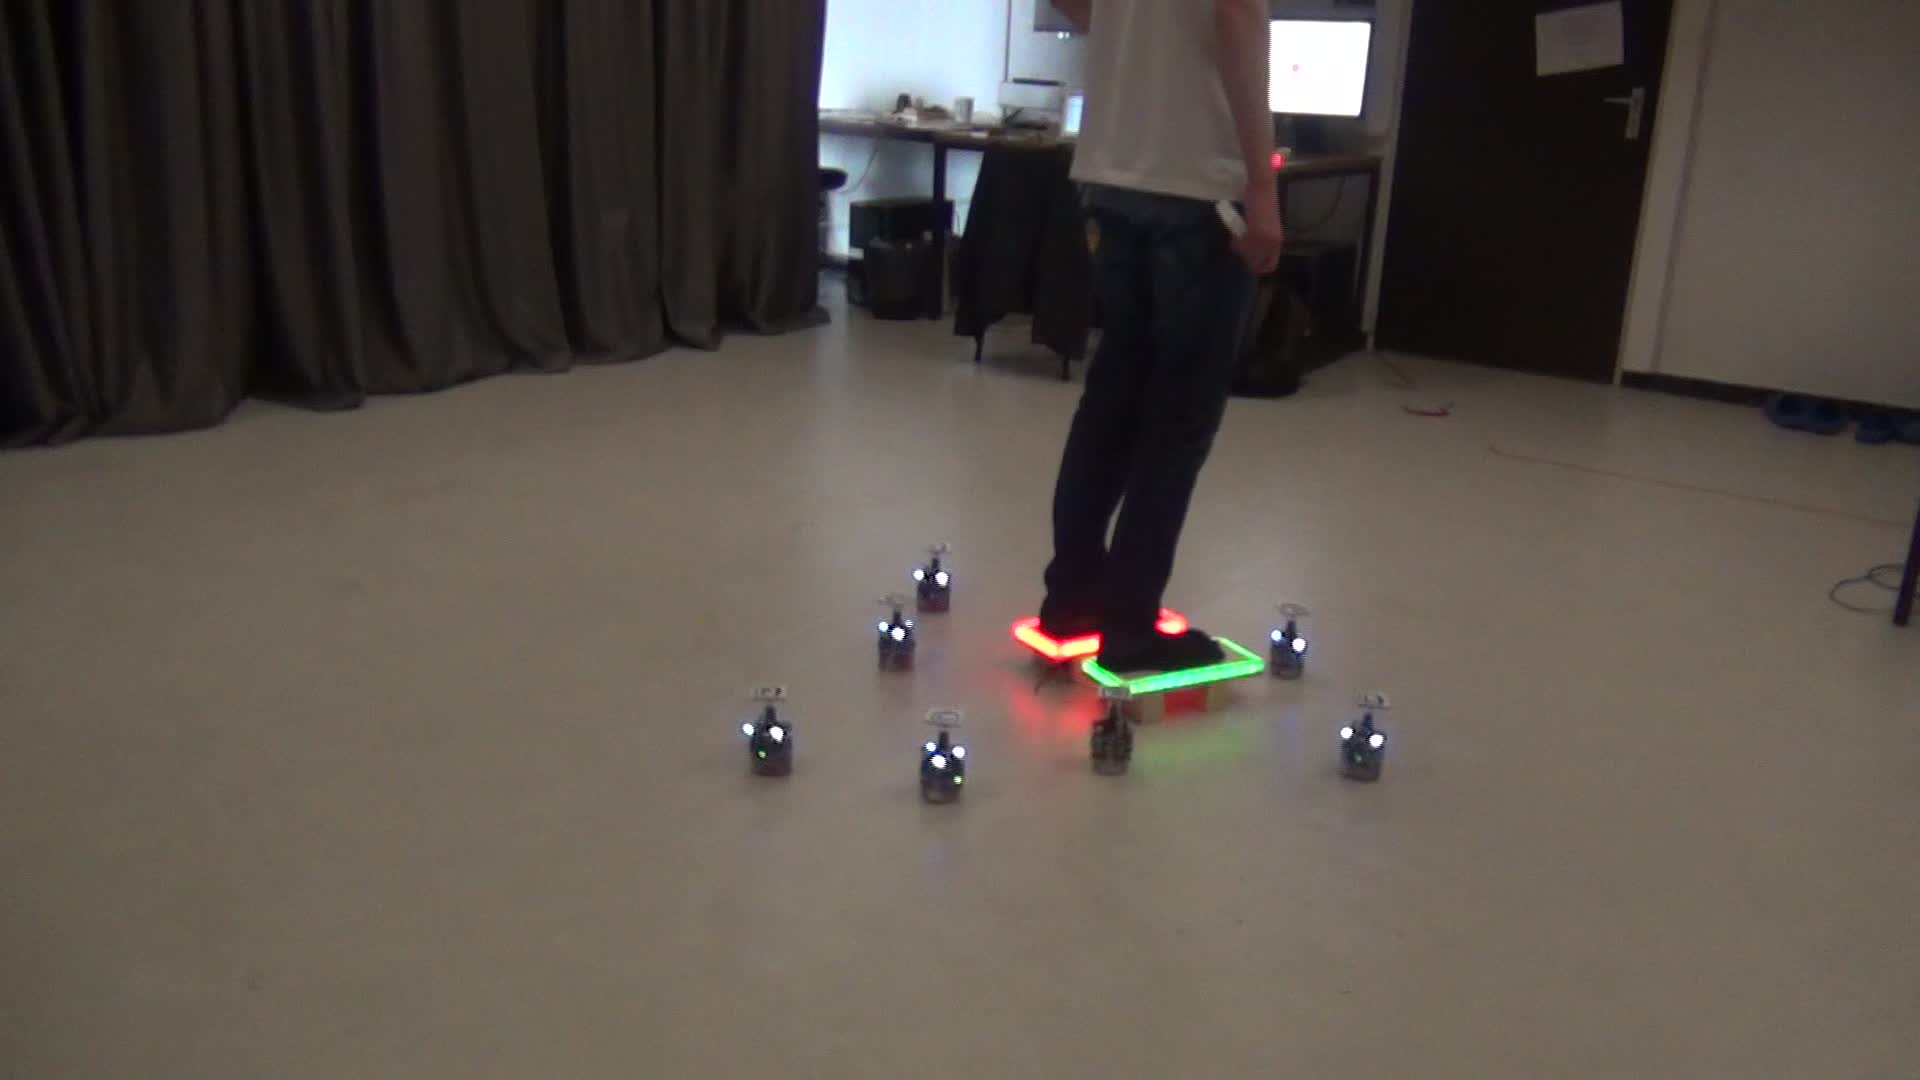
\includegraphics[width=\textwidth]{images/vlcsnap-00005.jpg}
					\centering (d)
				\end{minipage}
				\begin{minipage}[c]{0.49\textwidth}
					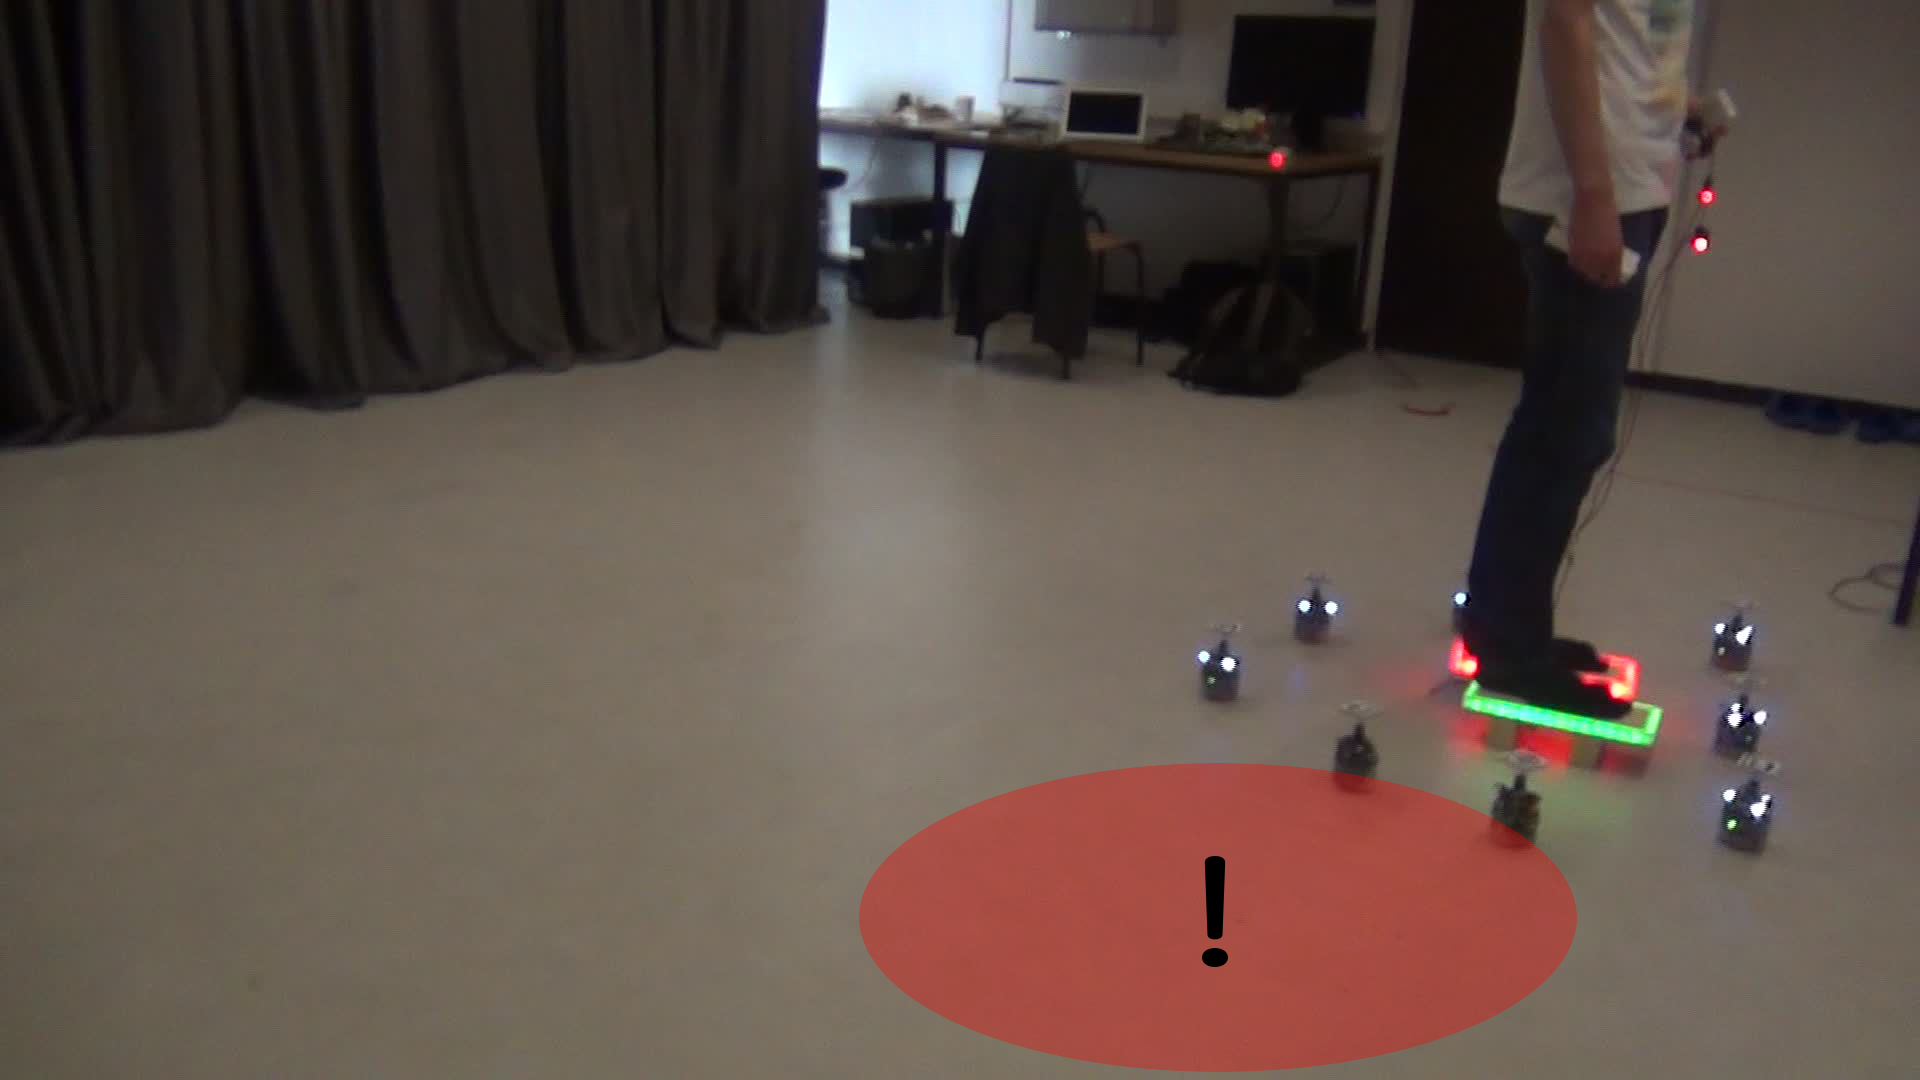
\includegraphics[width=\textwidth]{images/vlcsnap-00007.jpg}
					\centering (e)
				\end{minipage}
				
				
				\caption{I'm fabulous}{Captured from the video of the experiment. The virtual dangerous area is added as an overlay as a red disc.}
				\label{fig:demo_pictures}
			\end{figure}
			
			The experiment was a success. The robots notified the human about the dangerous area. They stayed on the boundary of the area. However, for some of the robots, the distance to the human was oscillating. One can see on Figure \ref{fig:demo_pictures} (b) that one of the robot on the back of the human is closer to the human than it should be. The speed of the human in this experiment was not constant. At the beginning, the human walked very slowly to the dangerous area. Then, he progressively increased the speed. The final speed was still low, though. For a real life application, the robots would have to be further from the human and form a wider circle. This would allow a higher anticipation, and higher walking speeds as the robots would have larger margins to react to the human changes of direction and speed. This experiment must be seen as a proof of concept. Further development must be undertaken to obtain a system ready for real life applications.
	

\chapter{Conclusion}
	\begin{comment}
		I've done this, this and this (~1/2 pages). (Intro: "I'll do this, this...) \textcolor{red}{Put sentences of type "so what?". Continuous text. Limitations...}
			- Device that allow detection by robots
			- New type of protection: swarm protection in dangerous environments
			- Use of virtual physics for a pattern formation mechanism
			
		- Done this and this (Requirements, design, implementation with trial and error and a lot of debugging, hardware, experiments, analysis, report)
		- Limitations (speed, scope of the omnidirectional camera, flat surfaces, sensitive to light conditions, batteries). --> proof of concept
		- Future works
	\end{comment}
	
	In this chapter, we express our conclusions on our solution. The project followed a standard process. First, meetings were organised to capture the requirements of the final solution, the idea behind the project. In the weeks that followed, we came up with a design that was meeting the first requirements and heading in the right direction. Once the design was accepted, the implementation could begin. The implementation consisted in a trial and error process with a lot of debugging. The controller we implemented was incrementally updated and tested, first in the simulator then on the real robots. At the end, when we were only changing the details of the solution, the tests were only made on the real robots. In the meantime, the hardware needed to perform the experiment was built. Once the current solution was apparently meeting the initial expectations, the writing of the report started. The experiments evaluating the behaviour of the swarm with defined metrics started at the same time (see Chapter \ref{chap:experiments}). Afterwards came the analysis of the results.
	
	The idea behind the project was to create a new kind of protection with the expertise in swarm robotics we have in the laboratory. We decided to use the E-pucks \citep{mondada2009puck} to form a swarm encircling a human. The swarm is thus augmenting the capabilities of the human. He/she is able to \enquote{see} dangers that one usually cannot see. For this to happen, we implemented a controller for the individual robots composing the swarm. The controller is based on the principles of virtual physics and pattern formation. We had to think about how the robots would detect the human. The decision was made to build a portable device for this purpose. We built shoes with coloured LEDs that the robots can detect. Our solution was used in proof-of-concept experiment that yielded good results.
	 
	 
	I've done this and this for the solution (the solution is composed of...). It works.

	\paragraph{Future Works}
	[The future works that would be interesting from my point of view.]
	
		\subparagraph{Other Robots}
		\subparagraph{Guidance}
			
			\begin{description}
				\item[Zero Visibility Areas or Blind People:]
				\item[Human Motion Synchronisation:]
				\item[Vehicle Guidance:]
			\end{description}
			

%%%%%%%%%%%%%%%%%%%%%%%%%%%%%%%%%%%%%%%%%%%%%%%%%%%%%%%
% APPENDICES
%%%%%%%%%%%%%%%%%%%%%%%%%%%%%%%%%%%%%%%%%%%%%%%%%%%%%%%
\part*{Appendices}
\addcontentsline{toc}{part}{Appendices}
\appendix

%http://tex.stackexchange.com/questions/172496/adding-appendix-chapters-without-sections-in-table-of-contents

\chapter{E-puck}

\chapter{ARGoS}

\chapter{Arena Tracking System}
\label{app:arena_tracking_system}

\chapter{Range and Bearing}

\chapter{Omnidirectional Camera}

\chapter{Controller Code}

\textbf{TODO Put link to code in the text.}

\chapter{MATLAB Scripts Code}

\textbf{TODO Put link to code in the text.}

\chapter{Human Detection Devices Blueprints}

\backmatter
\newpage

%%%%%%%%%%%%%%%%%%%%%%%%%%%%%%%%%%%%%%%%%%%%%%%%%%%%%%%
% BIBLIOGRAPHY
%%%%%%%%%%%%%%%%%%%%%%%%%%%%%%%%%%%%%%%%%%%%%%%%%%%%%%%
\addcontentsline{toc}{part}{Bibliography}
\part*{Bibliography}

\begin{filecontents}{thesis.bib}
%http://en.wikibooks.org/wiki/LaTeX/Bibliography_Management

@inproceedings{podevijn2012self,
  title={Self-organised feedback in human swarm interaction},
  author={Podevijn, Ga{\"e}tan and O’Grady, Rehan and Dorigo, Marco},
  booktitle={Proceedings of the workshop on robot feedback in human-robot interaction: how to make a robot readable for a human interaction partner (Ro-Man 2012)},
  year={2012}
}

@incollection{podevijn2014gesturing,
  title={Gesturing at subswarms: Towards direct human control of robot swarms},
  author={Podevijn, Ga{\"e}tan and O’Grady, Rehan and Nashed, Youssef SG and Dorigo, Marco},
  booktitle={Towards Autonomous Robotic Systems},
  pages={390--403},
  year={2014},
  publisher={Springer}
}

@article{brambilla2013swarm,
  title={Swarm robotics: a review from the swarm engineering perspective},
  author={Brambilla, Manuele and Ferrante, Eliseo and Birattari, Mauro and Dorigo, Marco},
  journal={Swarm Intelligence},
  volume={7},
  number={1},
  pages={1--41},
  year={2013},
  publisher={Springer}
}

@incollection{csahin2005swarm,
  title={Swarm robotics: From sources of inspiration to domains of application},
  author={{\c{S}}ahin, Erol},
  booktitle={Swarm robotics},
  pages={10--20},
  year={2005},
  publisher={Springer}
}

@phdthesis{kazadi2000swarm,
  title={Swarm engineering},
  author={Kazadi, Sanza T},
  year={2000},
  school={California Institute of Technology}
}

@book{minsky1967computation,
  title={Computation: finite and infinite machines},
  author={Minsky, Marvin L},
  year={1967},
  publisher={Prentice-Hall, Inc.}
}

@article{granovetter1978threshold,
  title={Threshold models of collective behavior},
  author={Granovetter, Mark},
  journal={American journal of sociology},
  pages={1420--1443},
  year={1978},
  publisher={JSTOR}
}

@inproceedings{bonabeau1997adaptive,
  title={Adaptive Task Allocation Inspired by a Model of Division of Labor in Social Insects.},
  author={Bonabeau, Eric and Sobkowski, Andrej and Theraulaz, Guy and Deneubourg, Jean-Louis},
  booktitle={BCEC},
  pages={36--45},
  year={1997}
}

@article{bachrach2010composable,
  title={Composable continuous-space programs for robotic swarms},
  author={Bachrach, Jonathan and Beal, Jacob and McLurkin, James},
  journal={Neural Computing and Applications},
  volume={19},
  number={6},
  pages={825--847},
  year={2010},
  publisher={Springer}
}

@article{wolpert1999introduction,
  title={An introduction to collective intelligence},
  author={Wolpert, David H and Tumer, Kagan},
  journal={arXiv preprint cs/9908014},
  year={1999}
}

@article{abbott2006emergence,
  title={Emergence explained: Abstractions: Getting epiphenomena to do real work},
  author={Abbott, Russ},
  journal={Complexity},
  volume={12},
  number={1},
  pages={13--26},
  year={2006},
  publisher={Wiley Online Library}
}

@article{pinciroli2012argos,
  title={{ARGoS}: a Modular, Parallel, Multi-Engine Simulator for Multi-Robot Systems},
  author={Carlo Pinciroli and Vito Trianni and Rehan O'Grady and Giovanni Pini and Arne Brutschy and Manuele Brambilla and Nithin Mathews and Eliseo Ferrante and Gianni {Di Caro} and Frederick Ducatelle and Mauro Birattari and Luca Maria Gambardella and Marco Dorigo},
  journal={Swarm intelligence},
  volume={6},
  number={4},
  pages={271--295},
  year={2012},
  publisher={Springer},
  address = {Berlin, Germany},
  doi = {10.1007/s11721-012-0072-5}
}

@inproceedings{daily2003world,
  title={World embedded interfaces for human-robot interaction},
  author={Daily, Mike and Cho, Youngkwan and Martin, Kevin and Payton, Dave},
  booktitle={System Sciences, 2003. Proceedings of the 36th Annual Hawaii International Conference on},
  pages={6--pp},
  year={2003},
  organization={IEEE}
}

@incollection{baizid2009human,
  title={Human multi-robots interaction with high virtual reality abstraction level},
  author={Baizid, Khelifa and Li, Zhao and Mollet, Nicolas and Chellali, Ryad},
  booktitle={Intelligent Robotics and Applications},
  pages={23--32},
  year={2009},
  publisher={Springer}
}

@inproceedings{mclurkin2006speaking,
  title={Speaking Swarmish: Human-Robot Interface Design for Large Swarms of Autonomous Mobile Robots.},
  author={McLurkin, James and Smith, Jennifer and Frankel, James and Sotkowitz, David and Blau, David and Schmidt, Brian},
  booktitle={AAAI Spring Symposium: To Boldly Go Where No Human-Robot Team Has Gone Before},
  pages={72--75},
  year={2006}
}

@inproceedings{mondada2009puck,
  title={The e-puck, a robot designed for education in engineering},
  author={Mondada, Francesco and Bonani, Michael and Raemy, Xavier and Pugh, James and Cianci, Christopher and Klaptocz, Adam and Magnenat, Stephane and Zufferey, Jean-Christophe and Floreano, Dario and Martinoli, Alcherio},
  booktitle={Proceedings of the 9th conference on autonomous robot systems and competitions},
  volume={1},
  number={LIS-CONF-2009-004},
  pages={59--65},
  year={2009},
  organization={IPCB: Instituto Polit{\'e}cnico de Castelo Branco}
}

@misc{wiki:001,
   author = "Wikipedia",
   title = "Geta (footwear) --- Wikipedia{,} The Free Encyclopedia",
   year = "2015",
   url = "http://en.wikipedia.org/w/index.php?title=Geta_(footwear)&oldid=651925222",
   note = "[Online; accessed 20-May-2015]"
 }
 
 @misc{ wiki:002,
   author = "Wikipedia",
   title = "Walking --- Wikipedia{,} The Free Encyclopedia",
   year = "2015",
   url = "https://en.wikipedia.org/w/index.php?title=Walking&oldid=671922191",
   note = "[Online; accessed 1-August-2015]"
 }
 
 @misc{ wiki:003,
   author = "Wikipedia",
   title = "Box plot --- Wikipedia{,} The Free Encyclopedia",
   year = "2015",
   url = "https://en.wikipedia.org/w/index.php?title=Box_plot&oldid=669188116",
   note = "[Online; accessed 5-August-2015]"
 }
 
 @article{khatib1986real,
  title={Real-time obstacle avoidance for manipulators and mobile robots},
  author={Khatib, Oussama},
  journal={The international journal of robotics research},
  volume={5},
  number={1},
  pages={90--98},
  year={1986},
  publisher={Sage Publications}
}

@article{reif1999social,
  title={Social potential fields: A distributed behavioral control for autonomous robots},
  author={Reif, John H and Wang, Hongyan},
  journal={Robotics and Autonomous Systems},
  volume={27},
  number={3},
  pages={171--194},
  year={1999},
  publisher={Elsevier}
}

@article{spears2004distributed,
  title={Distributed, physics-based control of swarms of vehicles},
  author={Spears, William M and Spears, Diana F and Hamann, Jerry C and Heil, Rodney},
  journal={Autonomous Robots},
  volume={17},
  number={2-3},
  pages={137--162},
  year={2004},
  publisher={Springer}
}

@inproceedings{gutierrez2009open,
  title={Open e-puck range \& bearing miniaturized board for local communication in swarm robotics},
  author={Guti{\'e}rrez, {\'A}lvaro and Campo, Alexandre and Dorigo, Marco and Donate, Jesus and Monasterio-Huelin, F{\'e}lix and Magdalena, Luis},
  booktitle={Robotics and Automation, 2009. ICRA'09. IEEE International Conference on},
  pages={3111--3116},
  year={2009},
  organization={IEEE}
}

@techreport{stranieri2013iridia,
  author={A. Stranieri and A.E. Turgut and M. Salvaro and L. Garattoni and G. Francesca and A. Reina and M. Dorigo and  M. Birattari},
  title={IRIDIA's Arena Tracking System},
  institution={IRIDIA, Universit{\'e} Libre de Bruxelles},
  year={2013},
  number={TR/IRIDIA/2013-013},
  address={Brussels, Belgium},
  month={January}
}

@incollection{reinaaugmented,
  author = {Reina, Andreagiovanni and Salvaro, Mattia and Francesca, Gianpiero and Garattoni, Lorenzo and Pinciroli, Carlo and Dorigo, Marco and Birattari, Mauro},
  title = {Augmented reality for robots: virtual sensing technology applied to a swarm of e-pucks},
  booktitle = {2015 {NASA/ESA} Conference on Adaptive Hardware and Systems ({AHS 2015}))},
  publisher = {{IEEE} Computer Society Press},
  address = {Los Alamitos, CA},
  year = {2015},
  pages = {1--6},
  note = {Paper ID sB\_p3}
}

@techreport{GarFraBruPinBir2015:techreport-004,
 author={L. Garattoni and G. Francesca and A. Brutschy and C. Pinciroli and M. Birattari},
 title={Software Infrastructure for E-puck (and TAM)},
 institution={IRIDIA, Universit{\'e} Libre de Bruxelles},
 year={2015},
 number={TR/IRIDIA/2015-004},
 address={Brussels, Belgium},
 month={July}
}

\end{filecontents}

%\nocite{*}
\bibliographystyle{plainnat}
\bibliography{thesis}

\end{document}
